% !TeX program = xelatex
\documentclass[aspectratio=169,11pt]{beamer}

% -------------------------------------------------
% Packages
% -------------------------------------------------
\usepackage{kotex}
\usepackage{fontspec}
\usepackage{amsmath,amssymb,bm,mathtools}
\usepackage{booktabs,array}
\usepackage{xcolor}
\usepackage{colortbl}
\usepackage{tikz}
\usetikzlibrary{positioning,arrows.meta,calc,fit,decorations.pathreplacing}
\usepackage[most]{tcolorbox}
\usepackage{listings}
\usepackage{adjustbox}

% -------------------------------------------------
% Colors (same as the notes)
% -------------------------------------------------
\definecolor{deepblue}{RGB}{34,71,120}
\definecolor{softblue}{RGB}{239,246,253}
\definecolor{softgray}{RGB}{246,247,249}
\definecolor{softgreen}{RGB}{239,249,242}
\definecolor{softyellow}{RGB}{255,249,229}
\definecolor{codegray}{RGB}{248,248,248}

% -------------------------------------------------
% Beamer look
% -------------------------------------------------
\usetheme{default}
\usefonttheme[onlymath]{serif}
\setbeamertemplate{navigation symbols}{}
\setbeamersize{text margin left=8mm,text margin right=8mm}
\setbeamercolor{structure}{fg=deepblue}
\setbeamercolor{frametitle}{fg=deepblue}
\setbeamercolor{title}{fg=deepblue}
\setbeamerfont{frametitle}{size=\large,series=\bfseries}
\setbeamertemplate{itemize items}[circle]
\setbeamertemplate{enumerate items}[default]
\setbeamertemplate{frametitle}{%
  \vskip3mm
  {\usebeamerfont{frametitle}\usebeamercolor[fg]{frametitle}\insertframetitle\par}%
  \vskip1mm
  {\color{deepblue!45}\hrule height 0.6pt}%
  \vskip1mm}
\setbeamertemplate{footline}{%
  \hbox to\paperwidth{%
    \hspace*{8mm}{\color{black!45}\scriptsize 학습 관련 기술: 코드 읽기\ifx\insertsectionhead\empty\else\ \ $\cdot$\ \ \insertsectionhead\fi}%
    \hfill{\color{black!45}\scriptsize\insertframenumber\,/\,\inserttotalframenumber}\hspace*{8mm}}%
  \vskip2.5mm}
\setbeamertemplate{title page}{%
  \vfill
  \begin{center}
  {\color{deepblue}\Huge\bfseries\inserttitle\par}
  \vskip3mm
  {\color{deepblue!60}\rule{9cm}{0.8pt}\par}
  \vskip3mm
  {\large\insertsubtitle\par}
  \vskip8mm
  {\normalsize\insertdate\par}
  \end{center}
  \vfill}
\AtBeginSection[]{%
  \begin{frame}
  \vfill
  \centering
  {\color{deepblue!55}\Large\bfseries \insertsectionnumber\par}
  \vskip2mm
  {\color{deepblue}\LARGE\bfseries\insertsectionhead\par}
  \vskip3mm
  {\color{deepblue!50}\rule{7cm}{0.8pt}\par}
  \vfill
  \end{frame}}
\setlength{\leftmargini}{1.2em}
\addtobeamertemplate{itemize/enumerate body begin}{}{\setlength{\itemsep}{0.2ex}}
\setlength{\leftmarginii}{1.1em}

% -------------------------------------------------
% Boxes (same colors as the notes)
% -------------------------------------------------
\newtcolorbox{keybox}[1][]{colback=softblue,colframe=deepblue,boxrule=0.7pt,arc=2mm,
  title=#1,fonttitle=\bfseries\small,left=2mm,right=2mm,top=1mm,bottom=1mm,
  toptitle=0.5mm,bottomtitle=0.5mm}
\newtcolorbox{thinkbox}[1][]{colback=softyellow,colframe=orange!70!black,boxrule=0.6pt,arc=2mm,
  title=#1,fonttitle=\bfseries\small,left=2mm,right=2mm,top=1mm,bottom=1mm,
  toptitle=0.5mm,bottomtitle=0.5mm}
\newtcolorbox{remarkbox}[1][]{colback=softgray,colframe=black!45,boxrule=0.5pt,arc=2mm,
  title=#1,fonttitle=\bfseries\small,left=2mm,right=2mm,top=1mm,bottom=1mm,
  toptitle=0.5mm,bottomtitle=0.5mm}

% -------------------------------------------------
% Code style
% -------------------------------------------------
\lstdefinestyle{pythonstyle}{
  language=Python,
  backgroundcolor=\color{codegray},
  basicstyle=\ttfamily\fontsize{7.6}{8.6}\selectfont,
  keywordstyle=\bfseries\color{deepblue},
  commentstyle=\itshape\color{black!55},
  stringstyle=\color{black!75},
  numbers=none,
  frame=single,
  rulecolor=\color{black!25},
  breaklines=true,
  showstringspaces=false,
  tabsize=4,
  columns=fullflexible,
  keepspaces=true,
  aboveskip=1mm,
  belowskip=1mm
}
\lstset{style=pythonstyle}
% program output: no Python colors, light green background
\lstdefinestyle{outstyle}{style=pythonstyle,language={},backgroundcolor=\color{softgreen}}
% smaller code for long listings
\newcommand{\codesmall}{\ttfamily\fontsize{7.4}{8.3}\selectfont}
\newcommand{\codetiny}{\ttfamily\fontsize{6.8}{7.6}\selectfont}

% -------------------------------------------------
% Math commands (same as the notes)
% -------------------------------------------------
\newcommand{\R}{\mathbb{R}}
\newcommand{\vect}[1]{\bm{#1}}
\newcommand{\T}{^{\mathsf T}}
\newcommand{\pd}[2]{\frac{\partial #1}{\partial #2}}

\newcommand{\figcap}[1]{\par\vskip1mm{\centering\footnotesize\color{black!70}#1\par}}
\newcommand{\code}[1]{\texttt{#1}}

\graphicspath{{slides_figures/}}

\title{학습 관련 기술: 코드 읽기}
\subtitle{NumPy 모듈 조립 $\cdot$ 실험 코드 6개 $\cdot$ \texttt{mnist\_torch.py}}
\date{딥러닝개론및연습 $\cdot$ 2026년 2학기}

\begin{document}

% =================================================
\begin{frame}[plain]
\titlepage
\end{frame}

% =================================================
\begin{frame}{이번 시간의 핵심 질문}
\begin{keybox}[이번 시간의 핵심 질문]
\begin{itemize}
\item 최적화 기법, 가중치 초기화, 배치 정규화, 가중치 감소, 드롭아웃을 \textbf{코드로는} 어떻게 쓸까?
\item 따로따로 배운 기법들을 \textbf{한 프로그램에 모두} 넣으면 어떻게 될까?
\item 노트의 그래프들은 \textbf{어떤 실험}으로 만든 것이고, 공정한 비교를 위해 무엇을 맞췄을까?
\item 같은 프로그램을 PyTorch로 쓰면 무엇이 짧아지고, 무엇이 그대로일까?
\end{itemize}
\end{keybox}
\vskip2mm
\begin{center}
\large $\Rightarrow$ \textbf{우리가 만든 NumPy 모듈 $\to$ 최종 코드 $\to$ 실험 코드 $\to$ PyTorch}
\end{center}
\end{frame}

\begin{frame}{학습목표}
\begin{enumerate}
\item \code{optimizers.py}의 다섯 가지 갱신 규칙과 AdamW를 코드로 읽을 수 있다
\item \code{layers.py}에 새로 생긴 \code{BatchNormalization}, \code{Dropout}, 가중치 감소를 읽을 수 있다
\item 세 모듈을 조립한 최종 코드 \code{mnist\_numpy\_final.py}를 처음부터 끝까지 설명할 수 있다
\item 실험 코드 6개가 \textbf{무엇을 같게 두고 무엇만 바꾸는지} 설명할 수 있다
\item \code{mnist\_torch.py}를 NumPy 최종 코드와 한 줄씩 대응시킬 수 있다
\end{enumerate}
\end{frame}

\begin{frame}{목차}
\footnotesize
\tableofcontents
\end{frame}

% =================================================
\section{코드 지도}
% =================================================

\begin{frame}{\code{학습관련기술/code} 폴더의 구조}
\centering
\begin{adjustbox}{max width=\linewidth,max totalheight=0.6\textheight}
\begin{tikzpicture}[>=Latex,
  mod/.style={draw=deepblue,fill=softblue,rounded corners=3pt,align=center,font=\small,text width=30mm,minimum height=11mm},
  run/.style={draw=black!50,fill=softgray,rounded corners=3pt,align=center,font=\scriptsize,text width=40mm,minimum height=7mm},
  fin/.style={draw=orange!70!black,fill=softyellow,rounded corners=3pt,align=center,font=\small,text width=40mm,minimum height=11mm}]
\node[mod,text width=34mm] (d) at (0,2.2) {\code{mnist\_data.py}\\{\scriptsize 데이터}};
\node[mod,text width=34mm] (l) at (4.5,2.2) {\code{layers.py}\\{\scriptsize 계층, \code{MultiLayerNet}}};
\node[mod,text width=34mm] (o) at (9,2.2) {\code{optimizers.py}\\{\scriptsize 갱신 규칙}};
\node[fin] (f) at (4.5,0.3) {\code{mnist\_numpy\_final.py}\\{\scriptsize 최종 코드 (모두 조립)}};
\node[fin] (t) at (12.5,0.3) {\code{mnist\_torch.py}\\{\scriptsize 같은 신경망, PyTorch}};
\node[run] (r2) at (0.75,-1.5) {\code{weight\_init\_activation.py}};
\node[run] (r3) at (5.25,-1.5) {\code{mnist\_optimizer\_compare.py}};
\node[run] (r4) at (9.75,-1.5) {\code{mnist\_init\_compare.py}};
\node[run] (r5) at (0.75,-2.5) {\code{mnist\_batchnorm.py}};
\node[run] (r6) at (5.25,-2.5) {\code{mnist\_overfit.py}};
\node[run] (r7) at (9.75,-2.5) {\code{hyperparameter\_search.py}};
\draw[->,thick] (d) -- (f); \draw[->,thick] (l) -- (f); \draw[->,thick] (o) -- (f);
\draw[->,thick,black!50] (d.east) to[bend left=8] (t.north);
\draw[decorate,decoration={brace,amplitude=5pt,mirror}] (-1.5,-3.0) -- (12.0,-3.0)
  node[midway,below=5pt,font=\small] {실험 코드: 기법 하나씩 비교 (모듈을 import 해서 쓴다. \code{weight\_init\_activation.py}만 데이터를 쓰지 않는다)};
\end{tikzpicture}
\end{adjustbox}
\vskip2mm
\raggedright
\small
\begin{itemize}
\item \textbf{모듈} 3개: 다른 파일이 \code{import}해서 쓰는 부품. 실행해도 아무것도 출력하지 않는다
\item \textbf{최종 코드}: 모든 기법을 한 신경망에 넣었다. \textbf{실험 코드}: 기법 \textbf{하나만} 바꿔 가며 비교한다
\item 모든 실행 결과와 그림은 이번 슬라이드를 위해 이 컴퓨터에서 실제로 실행한 것이다
\end{itemize}
\end{frame}

\begin{frame}[fragile]{모든 파일에 공통인 세 가지}
\textbf{1. 그림 저장 폴더}
\begin{lstlisting}
FIG_DIR = os.path.join(os.path.dirname(os.path.abspath(__file__)), "..", "figures")
os.makedirs(FIG_DIR, exist_ok=True)
\end{lstlisting}
\small
\begin{itemize}
\item \code{\_\_file\_\_}: 지금 실행 중인 파일의 경로. \code{abspath} $\to$ 절대 경로, \code{dirname} $\to$ 그 폴더(\code{code})
\item \code{".."}: 한 단계 위 폴더. 결과: \code{학습관련기술/figures}. \textbf{어디서 실행해도} 같은 곳에 저장된다
\end{itemize}
\normalsize
\textbf{2. 난수 씨앗 두 번}
\begin{lstlisting}
np.random.seed(1)          # the SAME initial weights
net = MultiLayerNet(...)
np.random.seed(2)          # the SAME mini-batches
\end{lstlisting}
\small
\begin{itemize}
\item 비교하는 설정마다 \textbf{같은 초기 가중치}, \textbf{같은 미니배치 순서} $\to$ 결과의 차이는 바꾼 설정 \textbf{하나} 때문
\end{itemize}
\textbf{3. 학습 루프는 언제나 같다}: \code{loss} $\to$ \code{backward} $\to$ \code{optimizer.update(net.params, grads)}
\end{frame}

% =================================================
\section{모듈 1: \texttt{optimizers.py}}
% =================================================

\begin{frame}[fragile]{모든 최적화 기법의 공통 모양}
\begin{lstlisting}
class SGD:
    """W <- W - lr * dL/dW"""
    def __init__(self, lr=0.01):
        self.lr = lr

    def update(self, params, grads):
        for key in params:
            params[key] -= self.lr * grads[key]
\end{lstlisting}
\begin{itemize}
\item \code{\_\_init\_\_}: \textbf{하이퍼파라미터}(학습률 등)를 받아 저장
\item \code{update(params, grads)}: 두 딕셔너리는 \textbf{같은 키} (\code{"W1"}, \code{"B1"}, \code{"gamma1"}, \ldots)
\item \code{-=}: \textbf{제자리에서} 갱신 $\to$ 같은 배열을 쓰는 계층도 바뀐 값을 본다 (\code{=}로 쓰면 학습이 안 된다)
\item 모든 기법이 이 모양을 지키므로, 학습 코드에서는 \textbf{\code{optimizer = ...} 한 줄만} 바꾸면 된다
\item 식: $W \leftarrow W - \eta\,\partial L/\partial W$ \ ($\eta$: 학습률 \code{lr})
\end{itemize}
\end{frame}

\begin{frame}[fragile]{\code{Momentum}: 속도 $v$를 기억한다}
\begin{columns}[T,onlytextwidth]
\begin{column}{0.56\textwidth}
\begin{lstlisting}[basicstyle=\codesmall]
class Momentum:
    def __init__(self, lr=0.01, beta=0.9):
        self.lr = lr
        self.beta = beta
        self.v = None

    def update(self, params, grads):
        if self.v is None:          # velocity starts at 0
            self.v = {key: np.zeros_like(val)
                      for key, val in params.items()}
        for key in params:
            self.v[key] = self.beta * self.v[key] \
                          - self.lr * grads[key]
            params[key] += self.v[key]
\end{lstlisting}
\end{column}
\begin{column}{0.40\textwidth}
\footnotesize
\[
\begin{aligned}
v &\leftarrow \beta v - \eta\,\pd{L}{W}\\
W &\leftarrow W + v
\end{aligned}
\]
\begin{itemize}
\item \code{self.v = None}: 처음에는 매개변수의 모양을 \textbf{모른다}
\item 첫 \code{update}에서 \code{params}와 같은 키, 같은 모양의 $0$ 배열을 만든다
\item \textbf{딕셔너리 내포}: \code{\{키: 값 for ...\}}
\item \code{np.zeros\_like(val)}: \code{val}과 같은 모양의 $0$
\end{itemize}
\end{column}
\end{columns}
\small
\begin{itemize}
\item 기울기의 방향이 계속 같으면 $v$가 쌓여 빨라지고, 방향이 바뀌면 서로 상쇄되어 진동이 줄어든다
\end{itemize}
\end{frame}

\begin{frame}[fragile]{\code{AdaGrad}와 \code{RMSProp}: 매개변수마다 다른 학습률}
\begin{columns}[T,onlytextwidth]
\begin{column}{0.50\textwidth}
\begin{lstlisting}[basicstyle=\codesmall]
class AdaGrad:
    def update(self, params, grads):
        if self.h is None:
            self.h = {key: np.zeros_like(val)
                      for key, val in params.items()}
        for key in params:
            self.h[key] += grads[key] * grads[key]
            params[key] -= self.lr * grads[key] \
                / (np.sqrt(self.h[key]) + self.eps)
\end{lstlisting}
\small
\[
h \leftarrow h + g\odot g,\qquad
W \leftarrow W - \eta\,\frac{g}{\sqrt h+\varepsilon}
\]
\end{column}
\begin{column}{0.47\textwidth}
\begin{lstlisting}[basicstyle=\codesmall]
class RMSProp:
    def update(self, params, grads):
        ...
        for key in params:
            self.h[key] = self.rho * self.h[key] \
                + (1 - self.rho) * grads[key] * grads[key]
            params[key] -= self.lr * grads[key] \
                / (np.sqrt(self.h[key]) + self.eps)
\end{lstlisting}
\small
\[
h \leftarrow \rho h + (1-\rho)\, g\odot g
\]
\end{column}
\end{columns}
\vskip1mm
\small
\begin{itemize}
\item $g=\partial L/\partial W$. \code{grads[key] * grads[key]}: \textbf{원소별} 제곱 ($g\odot g$)
\item 많이 움직인 원소일수록 $h$가 커져서 그 원소의 걸음이 작아진다. \code{eps}$=10^{-7}$: $0$으로 나누기 방지
\item AdaGrad는 $h$가 \textbf{계속 커지기만} 해서 결국 멈춘다. RMSProp은 옛 기울기를 잊는다 (지수이동평균)
\end{itemize}
\end{frame}

\begin{frame}[fragile]{\code{Adam}: Momentum + RMSProp + 편향 보정}
\begin{columns}[T,onlytextwidth]
\begin{column}{0.56\textwidth}
\begin{lstlisting}[basicstyle=\codetiny]
class Adam:
    def __init__(self, lr=0.001, beta1=0.9,
                 beta2=0.999, eps=1e-8):
        ...
        self.k = 0
        self.m = None
        self.v = None

    def update(self, params, grads):
        if self.m is None:
            self.m = {key: np.zeros_like(val) for ...}
            self.v = {key: np.zeros_like(val) for ...}
        self.k += 1
        for key in params:
            self.m[key] = self.beta1 * self.m[key] \
                + (1 - self.beta1) * grads[key]
            self.v[key] = self.beta2 * self.v[key] \
                + (1 - self.beta2) * grads[key] ** 2
            m_hat = self.m[key] / (1 - self.beta1 ** self.k)
            v_hat = self.v[key] / (1 - self.beta2 ** self.k)
            params[key] -= self.lr * m_hat \
                / (np.sqrt(v_hat) + self.eps)
\end{lstlisting}
\end{column}
\begin{column}{0.40\textwidth}
\footnotesize
\[
\begin{aligned}
m &\leftarrow \beta_1 m + (1-\beta_1) g\\
v &\leftarrow \beta_2 v + (1-\beta_2) g\odot g\\
\hat m &= m/(1-\beta_1^k),\ \ \hat v = v/(1-\beta_2^k)\\
W &\leftarrow W - \eta\,\frac{\hat m}{\sqrt{\hat v}+\varepsilon}
\end{aligned}
\]
\begin{itemize}
\item $m$: 기울기의 평균 (Momentum 역할)
\item $v$: 기울기 제곱의 평균 (RMSProp 역할)
\item \code{self.k}: 지금까지의 갱신 횟수
\item 편향 보정: $m$, $v$가 $0$에서 출발해 처음에 너무 작은 것을 바로잡는다
\end{itemize}
\end{column}
\end{columns}
\end{frame}

\begin{frame}[fragile]{\code{AdamW}: 상속으로 한 줄만 더한다}
\begin{lstlisting}[basicstyle=\codesmall]
class AdamW(Adam):
    """Adam + decoupled weight decay:  W <- W - lr * (m_hat / (sqrt(v_hat) + eps) + wd * W)
       The decay does NOT go through m and v.  Only weights (keys "W1", "W2", ...) are decayed."""
    def __init__(self, lr=0.001, beta1=0.9, beta2=0.999, eps=1e-8, weight_decay=0.01):
        super().__init__(lr, beta1, beta2, eps)
        self.weight_decay = weight_decay

    def update(self, params, grads):
        for key in params:
            if key.startswith("W"):
                params[key] -= self.lr * self.weight_decay * params[key]   # shrink W
        super().update(params, grads)                    # the usual Adam step
\end{lstlisting}
\begin{itemize}
\item \code{class AdamW(Adam)}: Adam을 \textbf{상속}. \code{super()}는 부모 클래스(Adam)를 부른다
\item 먼저 $W \leftarrow W - \eta\lambda W$ (가중치를 조금 \textbf{줄이고}), 그다음 보통의 Adam 한 걸음
\item \code{key.startswith("W")}: 가중치 행렬만. 편향 \code{B}, BatchNorm의 \code{gamma}, \code{beta}는 줄이지 않는다
\end{itemize}
\end{frame}

\begin{frame}{Adam + L2와 AdamW는 무엇이 다른가}
\centering
\small
\renewcommand{\arraystretch}{1.4}
\begin{tabular}{>{\raggedright}p{3.0cm}>{\raggedright}p{4.8cm}>{\raggedright\arraybackslash}p{4.8cm}}
\toprule
& \textbf{Adam + L2} & \textbf{AdamW} \\
\midrule
감소를 넣는 곳 & 손실: $L+\frac\lambda2\sum\|W\|^2$ & 갱신: $W\leftarrow W-\eta\lambda W$ \\
코드 & {\footnotesize\code{MultiLayerNet(}\ \code{\ \ weight\_decay\_lambda=...)}\ + \code{Adam(...)}} & {\footnotesize\code{MultiLayerNet()}\ + \code{AdamW(}\ \code{\ \ weight\_decay=...)}} \\
감소 항 $\lambda W$의 길 & 기울기에 더해져 $m$, $v$를 거치고 $\sqrt{\hat v}$로 \textbf{나뉜다} & $m$, $v$ \textbf{밖에서} 따로 \\
결과 & 기울기가 큰 가중치일수록 감소가 \textbf{약해진다} & 모든 가중치가 같은 비율로 줄어든다 \\
\bottomrule
\end{tabular}
\raggedright
\begin{itemize}
\item SGD에서는 두 방법이 \textbf{같다}: $W - \eta(g+\lambda W) = (W-\eta\lambda W) - \eta g$
\item Adam에서는 나눗셈 때문에 달라진다. 실제 결과의 차이는 \code{mnist\_overfit.py}의 (5)에서 본다
\end{itemize}
\end{frame}

% =================================================
\section{모듈 2: \texttt{layers.py}의 새 부분}
% =================================================

\begin{frame}{\code{layers.py}: 무엇이 새로 생겼나}
\centering
\small
\renewcommand{\arraystretch}{1.25}
\begin{tabular}{>{\raggedright}p{4.2cm}>{\raggedright\arraybackslash}p{8.6cm}}
\toprule
\textbf{부분} & \textbf{내용} \\
\midrule
\code{Affine}, \code{Relu}, \code{Sigmoid}, softmax, 손실 계층 & \code{mnist\_mlp.py}와 같다 \\
\code{BatchNormalization} & \textbf{새로}: 미니배치마다 노드별로 정규화, 학습/추론이 다르다 \\
\code{Dropout} & \textbf{새로}: 학습 때 노드를 무작위로 끈다 \\
\code{MultiLayerNet} & \textbf{확장}: Xavier/He 초기화, BatchNorm과 Dropout 끼워 넣기, 가중치 감소, \code{train\_flg} \\
\bottomrule
\end{tabular}
\vskip3mm
\raggedright
\begin{itemize}
\item 신경망의 모양: \ Affine $\to$ (BatchNorm) $\to$ 활성화 $\to$ (Dropout) \ 를 은닉층 수만큼 반복 $\to$ Affine $\to$ Softmax-손실
\item 괄호 안의 계층은 인자로 켜고 끈다: \code{use\_batchnorm=True}, \code{use\_dropout=True}
\end{itemize}
\end{frame}

\begin{frame}[fragile]{\code{BatchNormalization} (1): 만들기}
\begin{lstlisting}
class BatchNormalization:
    """Normalize each node (column) over the mini-batch, then scale and shift:
       x_hat = (x - mu) / sqrt(var + eps),   y = gamma * x_hat + beta"""
    def __init__(self, gamma, beta, momentum=0.9, eps=1e-7):
        self.gamma = gamma          # (1, m)
        self.beta = beta            # (1, m)
        self.momentum = momentum
        self.eps = eps
        self.running_mean = None    # used at test time
        self.running_var = None
        self.dgamma = None
        self.dbeta = None
\end{lstlisting}
\begin{itemize}
\item \code{gamma}, \code{beta}: $(1,m)$. 노드마다 하나씩. \code{MultiLayerNet}이 만들어서 넘겨준다 (\code{params}에도 같은 배열)
\item \code{momentum=0.9}: 이동평균에서 \textbf{옛 값}의 비중. \code{eps}: $\sqrt{0}$이 되지 않게 더하는 작은 수
\item \code{running\_mean}, \code{running\_var}: 추론할 때 쓸 평균과 분산. 아직 노드 수를 모르므로 \code{None}
\end{itemize}
\end{frame}

\begin{frame}[fragile]{\code{BatchNormalization} (2): 순전파}
\begin{columns}[T,onlytextwidth]
\begin{column}{0.60\textwidth}
\begin{lstlisting}[basicstyle=\codetiny]
def forward(self, X, train_flg=True):
    if self.running_mean is None:
        self.running_mean = np.zeros((1, X.shape[1]))
        self.running_var = np.ones((1, X.shape[1]))
    if train_flg:                     # statistics of THIS mini-batch
        mu = np.mean(X, axis=0, keepdims=True)        # (1, m)
        xc = X - mu                                   # (h, m)
        var = np.mean(xc ** 2, axis=0, keepdims=True) # (1, m)
        std = np.sqrt(var + self.eps)
        xn = xc / std                                 # x_hat (h, m)
        self.h, self.xc, self.std, self.xn = X.shape[0], xc, std, xn
        self.running_mean = self.momentum * self.running_mean \
                            + (1 - self.momentum) * mu
        self.running_var = self.momentum * self.running_var \
                           + (1 - self.momentum) * var
    else:                             # test time: running averages
        xn = (X - self.running_mean) / np.sqrt(self.running_var + self.eps)
    return self.gamma * xn + self.beta
\end{lstlisting}
\end{column}
\begin{column}{0.36\textwidth}
\small
\[
\begin{aligned}
\mu &= \tfrac1h\textstyle\sum_n x_n\\
\sigma^2 &= \tfrac1h\textstyle\sum_n (x_n-\mu)^2\\
\hat x_n &= \dfrac{x_n-\mu}{\sqrt{\sigma^2+\varepsilon}}\\
y_n &= \gamma\,\hat x_n+\beta
\end{aligned}
\]
\begin{itemize}
\item \code{axis=0}: 미니배치 방향(\textbf{열마다}). 노드 하나에 평균 하나
\item 역전파에 쓸 \code{xc}, \code{std}, \code{xn}을 저장
\item $\gamma$, $\beta$: 학습하는 매개변수 (처음 $1$, $0$)
\end{itemize}
\end{column}
\end{columns}
\end{frame}

\begin{frame}{\code{BatchNormalization} (3): 학습할 때와 추론할 때}
\begin{columns}[T,onlytextwidth]
\begin{column}{0.48\textwidth}
\begin{keybox}[학습 (\code{train\_flg=True})]
\small
\begin{itemize}
\item \textbf{지금 미니배치}의 $\mu$, $\sigma^2$로 정규화
\item 동시에 이동평균을 갱신:
\[
\bar\mu \leftarrow 0.9\,\bar\mu + 0.1\,\mu
\]
\end{itemize}
\end{keybox}
\end{column}
\begin{column}{0.48\textwidth}
\begin{keybox}[추론 (\code{train\_flg=False})]
\small
\begin{itemize}
\item 학습 중에 모아 둔 $\bar\mu$, $\bar\sigma^2$로 정규화
\item 이미지 \textbf{한 장}만 넣어도 같은 답이 나온다
\item 이동평균은 바꾸지 않는다
\end{itemize}
\end{keybox}
\end{column}
\end{columns}
\vskip2mm
\small
\begin{itemize}
\item \code{running\_mean}, \code{running\_var}는 \textbf{학습으로 얻었지만 기울기로 갱신하지 않는 값}이다
\item 그래서 \code{params}에 들어 있지 \textbf{않다}. 계층 객체 안에만 있다
\item \code{running\_mean is None}: 처음 \code{forward}할 때 노드 수(\code{X.shape[1]})를 보고 만든다
\item 최종 코드에서 중요해진다: 신경망을 저장할 때 \code{params}만 복사하면 이동평균이 빠진다 (\code{get\_state})
\end{itemize}
\end{frame}

\begin{frame}[fragile]{\code{BatchNormalization} (4): 역전파}
\begin{columns}[T,onlytextwidth]
\begin{column}{0.58\textwidth}
\begin{lstlisting}[basicstyle=\codesmall]
def backward(self, dY):
    self.dbeta = np.sum(dY, axis=0, keepdims=True)
    self.dgamma = np.sum(self.xn * dY, axis=0, keepdims=True)
    dxn = self.gamma * dY
    dxc = dxn / self.std
    dstd = -np.sum(dxn * self.xc / (self.std * self.std),
                   axis=0, keepdims=True)
    dvar = 0.5 * dstd / self.std
    dxc += (2.0 / self.h) * self.xc * dvar
    dmu = np.sum(dxc, axis=0, keepdims=True)
    return dxc - dmu / self.h
\end{lstlisting}
\end{column}
\begin{column}{0.38\textwidth}
\small
계산 그래프를 거꾸로:
\begin{enumerate}
\item $y=\gamma\hat x+\beta$: \code{dbeta}, \code{dgamma}, \code{dxn}
\item $\hat x = x_c/\sigma$: $x_c$와 $\sigma$ 두 갈래
\item $\sigma=\sqrt{\sigma^2+\varepsilon}$: \code{dvar}
\item $\sigma^2=\frac1h\sum x_c^2$: \code{dxc}에 더함
\item $x_c = x-\mu$: \code{dmu}를 빼서 \code{dX}
\end{enumerate}
\end{column}
\end{columns}
\small
\begin{itemize}
\item \code{dbeta}, \code{dgamma}는 $\beta$, $\gamma$의 모양 $(1,m)$이 되도록 행 방향으로 더한다 (Affine의 \code{dB}와 같은 이유)
\item $x$는 $x_c$로 직접, 그리고 $\mu$와 $\sigma^2$를 거쳐서 \textbf{여러 경로}로 손실에 영향 $\to$ 모든 경로의 기울기를 더한다
\item 식의 유도는 노트의 배치 정규화 절. 이 역전파가 맞는지는 \code{mnist\_batchnorm.py}의 기울기 검사로 확인한다
\end{itemize}
\end{frame}

\begin{frame}[fragile]{\code{Dropout}: 역(inverted) 드롭아웃}
\begin{columns}[T,onlytextwidth]
\begin{column}{0.56\textwidth}
\begin{lstlisting}[basicstyle=\codesmall]
class Dropout:
    def __init__(self, dropout_ratio=0.5):
        self.dropout_ratio = dropout_ratio
        self.mask = None

    def forward(self, X, train_flg=True):
        if train_flg:
            keep = 1.0 - self.dropout_ratio
            # *X.shape unpacks the shape tuple
            self.mask = (np.random.rand(*X.shape) < keep) / keep
            return X * self.mask
        return X

    def backward(self, dY):
        return dY * self.mask
\end{lstlisting}
\end{column}
\begin{column}{0.40\textwidth}
\small
\begin{itemize}
\item \code{np.random.rand}: $[0,1)$의 균등분포 난수
\item \code{< keep}: 확률 \code{keep}으로 \code{True}
\item \code{/ keep}: 살아남은 노드를 $\frac{1}{\text{keep}}$배 $\to$ 기댓값이 그대로
\item 그래서 추론할 때는 \textbf{아무것도 하지 않고} 그대로 통과
\item 역전파: 꺼진 노드는 기울기도 $0$
\end{itemize}
\end{column}
\end{columns}
\small
\begin{itemize}
\item \code{*X.shape}: 튜플을 풀어서 인자로. \code{X.shape}가 \code{(100, 50)}이면 \code{rand(100, 50)}
\item \code{mask}의 값은 $0$ 또는 $1/\text{keep}$ (예: 비율 $0.2$이면 $0$ 또는 $1.25$)
\item PyTorch의 \code{nn.Dropout}과 같은 방식이다
\end{itemize}
\end{frame}

\begin{frame}[fragile]{\code{MultiLayerNet} (1): 인자와 가중치 초기화}
\begin{lstlisting}[basicstyle=\codetiny]
def __init__(self, input_size, hidden_sizes, output_size,
             activation="relu", loss="ce", weight_init_std=0.05, use_batchnorm=False,
             weight_decay_lambda=0.0, use_dropout=False, dropout_ratio=0.5):
    sizes = [input_size] + list(hidden_sizes) + [output_size]   # e.g. [784, 256, 128, 10]
    self.weight_decay_lambda = weight_decay_lambda
    ...
    for i in range(len(sizes) - 1):
        n_in, n_out = sizes[i], sizes[i + 1]
        if weight_init_std == "xavier":            # Var(W) = 1/n_in  (sigmoid, tanh)
            std = np.sqrt(1.0 / n_in)
        elif weight_init_std == "he":              # Var(W) = 2/n_in  (ReLU)
            std = np.sqrt(2.0 / n_in)
        else:                                      # a fixed number, e.g. 0.01
            std = weight_init_std
        W = std * np.random.randn(n_in, n_out)     # (input nodes, output nodes)
\end{lstlisting}
\footnotesize
\begin{itemize}
\item 새 인자: \code{use\_batchnorm}, \code{weight\_decay\_lambda}($\lambda$), \code{use\_dropout}, \code{dropout\_ratio}. 기본값은 모두 ``끔''
\item \code{weight\_init\_std}: 숫자 또는 문자열 \code{"xavier"}, \code{"he"}. 표준편차는 \textbf{그 층의 입력 노드 수} \code{n\_in}으로 정한다
\[
\text{Xavier: } \sigma=\sqrt{1/n_{\text{in}}}\ \ (\text{sigmoid, tanh}),\qquad
\text{He: } \sigma=\sqrt{2/n_{\text{in}}}\ \ (\text{ReLU})
\]
\end{itemize}
\end{frame}

\begin{frame}[fragile]{\code{MultiLayerNet} (2): 계층 쌓기}
\begin{lstlisting}[basicstyle=\codesmall]
        B = np.zeros((1, n_out))
        self.params[f"W{i + 1}"] = W
        self.params[f"B{i + 1}"] = B
        self.layers.append(Affine(W, B))
        if i < len(sizes) - 2:                     # hidden layer
            if use_batchnorm:                      # Affine -> BatchNorm -> activation
                gamma, beta = np.ones((1, n_out)), np.zeros((1, n_out))
                self.params[f"gamma{i + 1}"] = gamma
                self.params[f"beta{i + 1}"] = beta
                self.layers.append(BatchNormalization(gamma, beta))
            self.layers.append(Relu() if activation == "relu" else Sigmoid())
            if use_dropout:                        # ... -> activation -> Dropout
                self.layers.append(Dropout(dropout_ratio))
    self.last = SoftmaxWithCrossEntropy() if loss == "ce" else SoftmaxWithSquaredError()
\end{lstlisting}
\small
\begin{itemize}
\item 은닉층마다: Affine $\to$ (BatchNorm) $\to$ 활성화 $\to$ (Dropout). 마지막 Affine 뒤에는 아무것도 없다
\item $\gamma$, $\beta$도 \code{params}에 들어간다 $\to$ 최적화 기법이 $W$, $B$와 \textbf{똑같이} 갱신한다
\item \code{params}의 배열과 계층이 가진 배열은 \textbf{같은 객체} $\to$ 갱신은 반드시 제자리에서 (\code{-=})
\end{itemize}
\end{frame}

\begin{frame}[fragile]{\code{MultiLayerNet} (3): \code{predict}와 \code{train\_flg}}
\begin{lstlisting}
def predict(self, X, train_flg=False):    # scores U
    for layer in self.layers:
        if isinstance(layer, (BatchNormalization, Dropout)):   # training and test differ
            X = layer.forward(X, train_flg)
        else:
            X = layer.forward(X)
    return X

def accuracy(self, X, T):                 # used for evaluation: running statistics
    U = self.predict(X)
    return np.mean(np.argmax(U, axis=1) == np.argmax(T, axis=1))
\end{lstlisting}
\begin{itemize}
\item \code{train\_flg}의 기본값은 \code{False}(추론). 학습 때만 \code{loss}가 \code{True}로 부른다
\item \code{isinstance(layer, (A, B))}: A \textbf{또는} B의 객체인가. 이 두 계층만 \code{train\_flg}를 받는다
\item \code{accuracy}는 \code{predict(X)} $\to$ 항상 \textbf{추론 모드}: 이동평균 사용, 드롭아웃 끔
\item PyTorch에서는 이 \code{train\_flg}를 인자로 넘기지 않고 \code{model.train()} / \code{model.eval()}로 한 번에 정한다
\end{itemize}
\end{frame}

\begin{frame}[fragile]{\code{MultiLayerNet} (4): 손실에 가중치 감소 더하기}
\begin{lstlisting}
def loss(self, X, T):                     # used for training: batch statistics, dropout
    data_loss = self.last.forward(self.predict(X, train_flg=True), T)
    # weight decay: + (lambda/2) * sum of W^2 over all weight matrices (not B, gamma, beta)
    sum_W2 = sum(np.sum(W ** 2) for key, W in self.params.items() if key.startswith("W"))
    return data_loss + 0.5 * self.weight_decay_lambda * sum_W2
\end{lstlisting}
\[
L_{\text{total}} = L + \frac{\lambda}{2}\sum_{\ell}\|W_\ell\|^2,
\qquad \|W\|^2=\sum_{i,j} w_{ij}^2
\]
\begin{itemize}
\item \code{predict(X, train\_flg=True)}: 학습용 순전파. BatchNorm은 미니배치 통계, Dropout은 켜짐
\item \code{sum(... for ... if ...)}: 생성식. 키가 \code{W}로 시작하는 배열의 제곱합을 모두 더한다
\item $\lambda=0$(기본값)이면 원래 손실 그대로. 편향, $\gamma$, $\beta$는 감소시키지 않는다
\end{itemize}
\end{frame}

\begin{frame}[fragile]{\code{MultiLayerNet} (5): 기울기 모으기와 가중치 감소}
\begin{lstlisting}[basicstyle=\codesmall]
def backward(self):                       # call right after loss()
    d = self.last.backward()
    for layer in reversed(self.layers):   # the same rule, layer after layer
        d = layer.backward(d)
    grads, k = {}, 0
    ...
    for layer in self.layers:
        if isinstance(layer, Affine):
            k += 1
            grads[f"W{k}"], grads[f"B{k}"] = layer.dW, layer.dB
        elif isinstance(layer, BatchNormalization):
            grads[f"gamma{k}"], grads[f"beta{k}"] = layer.dgamma, layer.dbeta
    for key in grads:                     # weight decay: gradient + lambda * W
        if key.startswith("W"):
            grads[key] = grads[key] + self.weight_decay_lambda * self.params[key]
    return grads
\end{lstlisting}
\small
\begin{itemize}
\item \code{k}는 Affine을 만날 때 $1$ 증가 $\to$ 그 뒤의 BatchNorm 기울기도 \textbf{같은 번호} (\code{gamma1}, \code{beta1}, \ldots)
\item 가중치 감소의 기울기: \
$\displaystyle \pd{L_{\text{total}}}{W_\ell} = \pd{L}{W_\ell} + \lambda W_\ell$ \ $\to$ \code{grads[key] + lambda * W}
\end{itemize}
\end{frame}

% =================================================
\section{최종 코드: \texttt{mnist\_numpy\_final.py}}
% =================================================

\begin{frame}{최종 코드: 배운 기법을 한 신경망에}
\footnotesize
\centering
\small
\renewcommand{\arraystretch}{1.08}
\begin{tabular}{>{\raggedright}p{3.0cm}>{\raggedright}p{6.2cm}>{\raggedright\arraybackslash}p{3.0cm}}
\toprule
\textbf{기법} & \textbf{최종 코드에서} & \textbf{모듈} \\
\midrule
가중치 초기화 & He (\code{weight\_init\_std="he"}) & \code{layers.py} \\
배치 정규화 & \code{use\_batchnorm=True} & \code{layers.py} \\
드롭아웃 & 꺼 둠 (\code{use\_dropout=False}), 한 단어로 켤 수 있다 & \code{layers.py} \\
최적화 기법 & AdamW (\code{lr=0.001}) & \code{optimizers.py} \\
가중치 감소 & AdamW의 \code{weight\_decay=0.01} ($W$만) & \code{optimizers.py} \\
검증 데이터 & 검증 정확도가 가장 높은 epoch를 저장 & 최종 코드 \\
test & 마지막에 \textbf{한 번만} & 최종 코드 \\
\bottomrule
\end{tabular}
\vskip2mm
\raggedright
\begin{itemize}
\item 신경망: 은닉층 4개(100개씩), 미니배치 100, 15 epoch. \textbf{\code{mnist\_torch.py}와 같은 설정}으로 맞췄다
\item 새로 만든 파일이지만 새 계층이나 새 식은 없다. 세 모듈을 \textbf{조립}하고, 학습한 상태를 저장하는 함수 두 개만 더했다
\end{itemize}
\end{frame}

\begin{frame}[fragile]{1. import와 데이터}
\footnotesize
\begin{lstlisting}[basicstyle=\codetiny]
import os
import time
import copy
import numpy as np
import matplotlib.pyplot as plt

from mnist_data import load_mnist_split
from layers import MultiLayerNet, BatchNormalization
from optimizers import AdamW

x_train, t_train, x_val, t_val, x_test, t_test = load_mnist_split()   # 55000 / 5000 / 10000
print("train:", x_train.shape, " validation:", x_val.shape, " test:", x_test.shape)
\end{lstlisting}
\begin{lstlisting}[style=outstyle,basicstyle=\codetiny]
train: (55000, 784)  validation: (5000, 784)  test: (10000, 784)
\end{lstlisting}
\begin{itemize}
\item \code{from layers import ...}: 같은 폴더의 \code{layers.py}에서 클래스를 가져온다. 파일 이름 $=$ 모듈 이름
\item \code{BatchNormalization}도 가져오는 이유: 저장할 때 이 계층을 찾아야 한다 (뒤의 \code{get\_state})
\item \code{copy}: 딕셔너리를 통째로 복사하는 \code{copy.deepcopy}를 쓰려고
\item \code{load\_mnist\_split}: \code{mnist\_mlp.py}의 데이터 준비를 함수로 묶은 것. 여섯 개를 한꺼번에 돌려준다
\end{itemize}
\end{frame}

\begin{frame}[fragile]{2. 모델 만들기}
\begin{lstlisting}
np.random.seed(1)
net = MultiLayerNet(784, [100, 100, 100, 100], 10,
                    activation="relu", loss="ce", weight_init_std="he",
                    use_batchnorm=True, use_dropout=False, dropout_ratio=0.2)
print("layers:", " -> ".join(type(layer).__name__ for layer in net.layers))
print("number of parameters:", net.num_params())
\end{lstlisting}
\begin{lstlisting}[style=outstyle,basicstyle=\codetiny]
layers: Affine -> BatchNormalization -> Relu -> Affine -> BatchNormalization -> Relu -> Affine ->
        BatchNormalization -> Relu -> Affine -> BatchNormalization -> Relu -> Affine
number of parameters: 110610
\end{lstlisting}
\small
\begin{itemize}
\item \code{" -> ".join(...)}: 문자열들을 \code{" -> "}로 이어 붙인다. \code{type(layer).\_\_name\_\_}: 클래스 이름
\item 매개변수 수: \
$\underbrace{784\cdot100+100}_{\text{Affine 1}}+\underbrace{3(100\cdot100+100)}_{\text{Affine 2--4}}+\underbrace{100\cdot10+10}_{\text{Affine 5}}+\underbrace{4\cdot(100+100)}_{\gamma,\ \beta}=110610$
\item 드롭아웃을 켜려면 \code{use\_dropout=True}로 바꾸기만 하면 된다. 이때 비율은 \code{0.2}
\end{itemize}
\end{frame}

\begin{frame}[fragile]{3. 최적화 기법: 한 줄}
\begin{lstlisting}
optimizer = AdamW(lr=0.001, weight_decay=0.01)   # decays only the weights W1, W2, ...
\end{lstlisting}
\begin{itemize}
\item \code{optimizer.update(net.params, grads)}를 부를 때마다
\begin{enumerate}
\item $W \leftarrow W - 0.001\times0.01\times W$ \ (\code{"W1"}, \ldots, \code{"W5"}만)
\item 모든 매개변수(\code{W}, \code{B}, \code{gamma}, \code{beta})에 Adam 한 걸음
\end{enumerate}
\item \code{MultiLayerNet}의 \code{weight\_decay\_lambda}는 기본값 $0$ 그대로 둔다 $\to$ 손실에는 감소 항이 \textbf{없다}
\item 다른 기법과 비교하려면 이 줄만 바꾼다: \code{SGD(lr=0.01)}, \code{Momentum(lr=0.01)}, \code{Adam(lr=0.001)}, \ldots
\end{itemize}
\begin{remarkbox}
\small 감소를 손실과 AdamW 양쪽에 넣으면 \textbf{두 번} 줄어든다. 한쪽에만 넣는다.
\end{remarkbox}
\end{frame}

\begin{frame}[shrink,fragile]{4. 학습한 상태 저장하기: \code{get\_state}}
\small
\begin{lstlisting}
def get_state(net):
    state = {"params": copy.deepcopy(net.params), "bn": []}
    for layer in net.layers:
        if isinstance(layer, BatchNormalization):
            state["bn"].append((layer.running_mean.copy(), layer.running_var.copy()))
    return state
\end{lstlisting}
\begin{itemize}
\item 신경망이 학습으로 얻은 것은 \textbf{두 종류}:
\begin{enumerate}
\item \code{params}: $W$, $B$, $\gamma$, $\beta$ (기울기로 갱신)
\item 각 BatchNorm 계층의 \code{running\_mean}, \code{running\_var} (이동평균, \code{params}에 \textbf{없다})
\end{enumerate}
\item \code{copy.deepcopy}: 딕셔너리 \textbf{안의 배열까지} 새로 복사. 그냥 \code{dict(net.params)}면 배열은 같은 객체라서 학습이 계속되면 함께 바뀐다
\item \code{.copy()}: NumPy 배열 하나를 복사
\end{itemize}
\begin{thinkbox}[이동평균을 빠뜨리면?]
\small 가장 좋았던 epoch의 $W$에 \textbf{마지막} epoch의 이동평균이 붙는다. 둘이 맞지 않아 정확도가 달라질 수 있다.
\end{thinkbox}
\end{frame}

\begin{frame}[fragile]{4. 저장한 상태 되돌리기: \code{set\_state}}
\begin{lstlisting}
def set_state(net, state):
    for key in net.params:
        net.params[key][...] = state["params"][key]      # IN PLACE: the layers share these arrays
    bn_layers = [layer for layer in net.layers if isinstance(layer, BatchNormalization)]
    for layer, (mean, var) in zip(bn_layers, state["bn"]):
        layer.running_mean, layer.running_var = mean.copy(), var.copy()
\end{lstlisting}
\begin{itemize}
\item \code{net.params[key][...] = 값}: 배열의 \textbf{내용만} 바꾼다 (\code{[...]}는 ``모든 원소'')
\begin{itemize}
\item \code{net.params[key] = 값}으로 쓰면 딕셔너리만 새 배열을 가리키고, \code{Affine} 계층은 \textbf{옛 배열}을 계속 쓴다
\item 학습 코드에서 \code{-=}를 써야 했던 것과 같은 이유
\end{itemize}
\item \code{[layer for ... if ...]}: 리스트 내포. BatchNorm 계층만 골라 순서대로
\item \code{zip}: BatchNorm 계층과 저장한 \code{(mean, var)}를 짝지어 하나씩
\end{itemize}
\end{frame}

\begin{frame}[shrink,fragile]{5. 학습 루프}
\small
\begin{lstlisting}[basicstyle=\codesmall]
epochs = 15
batch_size = 100
N = x_train.shape[0]
iter_per_epoch = N // batch_size

np.random.seed(2)                                 # mini-batch order (and dropout masks)
history = {"loss": [], "train": [], "val": []}
best_val, best_epoch, best_state = 0.0, 0, None
for epoch in range(1, epochs + 1):
    perm = np.random.permutation(N)
    total_loss = 0.0
    for it in range(iter_per_epoch):
        idx = perm[it * batch_size:(it + 1) * batch_size]
        loss = net.loss(x_train[idx], t_train[idx])   # forward (batch statistics, dropout on)
        grads = net.backward()                        # backward through every layer
        optimizer.update(net.params, grads)           # AdamW step
        total_loss += loss
    history["loss"].append(total_loss / iter_per_epoch)
    history["train"].append(net.accuracy(x_train, t_train))   # running statistics, dropout off
    history["val"].append(net.accuracy(x_val, t_val))
    print(...)
    if history["val"][-1] > best_val:             # keep the epoch with the best VALIDATION accuracy
        best_val, best_epoch = history["val"][-1], epoch
        best_state = get_state(net)
\end{lstlisting}
\end{frame}

\begin{frame}[shrink]{5. 학습 루프: 한 줄씩}
\small
\small
\begin{itemize}
\item \code{range(1, epochs + 1)}: epoch 번호를 $1$부터 $15$까지 (출력과 그림에 그대로 쓰려고)
\item \code{np.random.seed(2)}: 미니배치 순서를 고정 $\to$ 실행할 때마다 같은 결과
\item 미니배치 하나: \code{loss} $\to$ \code{backward} $\to$ \code{update}. \textbf{이 세 줄은 모든 실험 코드에서 같다}
\begin{itemize}
\item \code{net.loss}: \code{train\_flg=True}로 순전파 (BatchNorm은 이 미니배치의 통계, 이동평균 갱신)
\end{itemize}
\item \code{total\_loss / iter\_per\_epoch}: \textbf{epoch 평균} 손실 (마지막 미니배치 하나보다 덜 들쭉날쭉하다)
\item \code{net.accuracy}: 추론 모드 (이동평균). 훈련 데이터 $55000$장 \textbf{전체}와 검증 데이터 $5000$장
\item \code{if history["val"][-1] > best\_val}: 검증 정확도가 \textbf{지금까지 최고}이면 그 순간의 상태를 저장
\begin{itemize}
\item 학습이 끝난 뒤의 신경망이 아니라 \textbf{가장 좋았던 순간}의 신경망을 쓰기 위해서
\item 고르는 기준은 \textbf{검증} 데이터. test 데이터는 아직 한 번도 보지 않았다
\end{itemize}
\end{itemize}
\begin{keybox}
\small 이것도 일종의 \textbf{조기 종료}(early stopping): ``몇 epoch까지 학습할까''라는 하이퍼파라미터를 검증 데이터로 고른다.
\end{keybox}
\end{frame}

\begin{frame}[fragile]{5. 실행 결과}
\begin{lstlisting}[style=outstyle,basicstyle=\codesmall]
epoch  1 | loss 0.2918 | train acc 0.9732 | val acc 0.9646 (11s)
epoch  2 | loss 0.1116 | train acc 0.9840 | val acc 0.9768 (18s)
epoch  3 | loss 0.0749 | train acc 0.9889 | val acc 0.9758 (25s)
epoch  4 | loss 0.0593 | train acc 0.9915 | val acc 0.9786 (33s)
epoch  5 | loss 0.0470 | train acc 0.9929 | val acc 0.9770 (40s)
epoch  6 | loss 0.0393 | train acc 0.9937 | val acc 0.9782 (48s)
epoch  7 | loss 0.0339 | train acc 0.9951 | val acc 0.9798 (55s)
epoch  8 | loss 0.0295 | train acc 0.9946 | val acc 0.9750 (63s)
epoch  9 | loss 0.0289 | train acc 0.9960 | val acc 0.9808 (71s)
epoch 10 | loss 0.0273 | train acc 0.9945 | val acc 0.9782 (78s)
epoch 11 | loss 0.0254 | train acc 0.9968 | val acc 0.9772 (85s)
epoch 12 | loss 0.0201 | train acc 0.9982 | val acc 0.9824 (92s)
epoch 13 | loss 0.0200 | train acc 0.9978 | val acc 0.9786 (99s)
epoch 14 | loss 0.0187 | train acc 0.9973 | val acc 0.9792 (106s)
epoch 15 | loss 0.0179 | train acc 0.9979 | val acc 0.9804 (111s)
\end{lstlisting}
\small
\begin{itemize}
\item \textbf{첫 epoch}에 이미 검증 정확도 $96.46\%$. \code{mnist\_mlp.py}(SGD, 은닉층 2개)는 10 epoch 뒤에 $97.38\%$였다
\item 훈련 정확도는 $99.8\%$까지 오르지만 검증 정확도는 $97.5$--$98.2\%$에서 오르내린다
\end{itemize}
\end{frame}

\begin{frame}[fragile]{6. test는 한 번만}
\begin{lstlisting}
set_state(net, best_state)
print(f"chosen epoch {best_epoch}: val acc {net.accuracy(x_val, t_val):.4f}, "
      f"test acc {net.accuracy(x_test, t_test):.4f}")
\end{lstlisting}
\begin{lstlisting}[style=outstyle]
chosen epoch 12: val acc 0.9824, test acc 0.9787
\end{lstlisting}
\begin{itemize}
\item 검증 정확도가 가장 높았던 epoch 12의 상태로 되돌린다
\item \code{set\_state}가 제대로 되었는지 확인: 되돌린 뒤 계산한 검증 정확도 $0.9824$가 epoch 12의 출력과 \textbf{같다}
\item 그리고 test 데이터를 \textbf{처음이자 마지막으로} 쓴다: $97.87\%$
\item 검증 정확도($98.24\%$)보다 조금 낮다. 검증 데이터로 \textbf{골랐기} 때문에 검증 정확도는 약간 낙관적이다
\end{itemize}
\end{frame}

\begin{frame}{7. 결과 그림: \code{numpy\_final.png}}
\centering
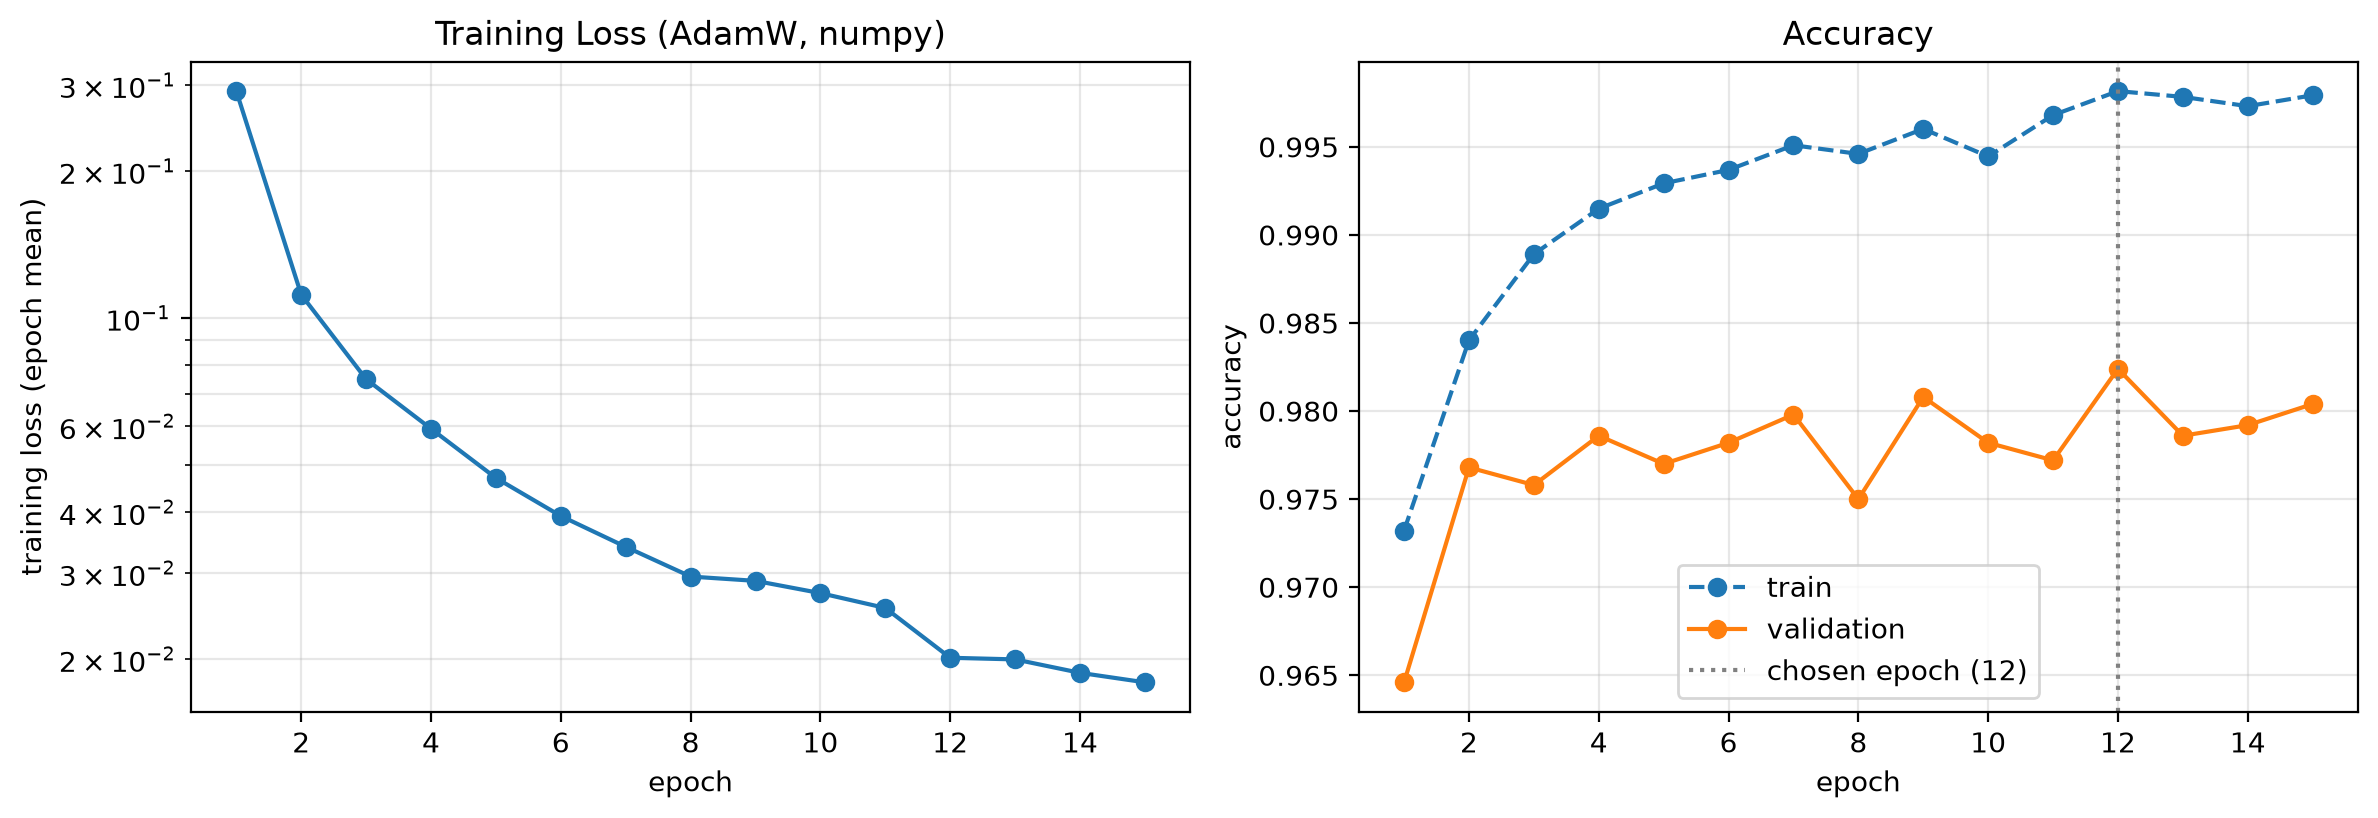
\includegraphics[width=0.86\linewidth]{numpy_final.png}
\figcap{왼쪽: epoch 평균 손실 (로그 축), 오른쪽: 훈련(점선)과 검증(실선) 정확도, 회색 점선: 고른 epoch}
\raggedright
\small
\begin{itemize}
\item 손실은 꾸준히 줄지만 검증 정확도는 epoch 4 이후 거의 제자리 $\to$ 더 오래 학습해도 크게 나아지지 않는다
\item 훈련과 검증의 차이(약 $1.5\%$p)를 더 줄이려면: 드롭아웃 켜기, 가중치 감소 키우기, 데이터 늘리기
\end{itemize}
\end{frame}

\begin{frame}[shrink,fragile]{그림 그리기 코드}
\small
\begin{lstlisting}[basicstyle=\codesmall]
fig, ax = plt.subplots(1, 2, figsize=(12, 4.2))
ax[0].plot(range(1, epochs + 1), history["loss"], "o-")
ax[0].set_yscale("log")
ax[0].set(xlabel="epoch", ylabel="training loss (epoch mean)", title="Training Loss (AdamW, numpy)")
ax[0].grid(True, which="both", alpha=0.3)
ax[1].plot(range(1, epochs + 1), history["train"], "o--", label="train")
ax[1].plot(range(1, epochs + 1), history["val"], "o-", label="validation")
ax[1].axvline(best_epoch, color="gray", linestyle=":", label=f"chosen epoch ({best_epoch})")
ax[1].set(xlabel="epoch", ylabel="accuracy", title="Accuracy")
ax[1].grid(True, alpha=0.3)
ax[1].legend()
fig.tight_layout()
fig.savefig(os.path.join(FIG_DIR, "numpy_final.png"), dpi=200, bbox_inches="tight")
plt.close(fig)
\end{lstlisting}
\small
\begin{itemize}
\item \code{plt.subplots(1, 2)}: 그림 하나에 축 두 개. \code{ax[0]}, \code{ax[1]}로 따로 그린다
\item \code{ax.set(xlabel=..., ylabel=..., title=...)}: 세 줄을 한 줄로. \code{set\_yscale("log")}: 로그 축
\item \code{"o-"}: 동그라미 + 실선, \code{"o--"}: 동그라미 + 점선. \code{axvline}: 세로선 하나
\item \code{grid(True, which="both")}: 로그 축의 작은 눈금에도 격자. \code{plt.close(fig)}: 메모리 정리
\end{itemize}
\end{frame}

% =================================================
\section{실험 1: \texttt{weight\_init\_activation.py}}
% =================================================

\begin{frame}[fragile]{무엇을 하는 코드인가}
\begin{itemize}
\item 층이 5개(100개씩)인 신경망에 무작위 입력 1000개를 \textbf{순전파만} 해서, 층마다 활성화값 $Z$의 \textbf{분포}를 본다
\item 학습은 하지 않는다. 바꾸는 것: 가중치의 표준편차, 활성화 함수
\item 활성화값이 $0$이나 $1$에 몰리거나(기울기 소실), 모두 같은 값이 되면(표현력 제한) 학습이 어렵다
\end{itemize}
\begin{lstlisting}
def sigmoid(a):
    return 1.0 / (1.0 + np.exp(-a))

def relu(a):
    return np.maximum(0.0, a)

def tanh(a):
    return np.tanh(a)
\end{lstlisting}
\begin{itemize}
\item 계층 클래스가 아니라 \textbf{함수}: 역전파가 필요 없으니 \code{forward}만 있으면 된다
\item \code{np.maximum(0.0, a)}: 원소마다 $0$과 비교해 큰 값 $=$ ReLU
\end{itemize}
\end{frame}

\begin{frame}[shrink,fragile]{\code{forward\_activations}: 층마다 $Z$를 모은다}
\small
\begin{lstlisting}
def forward_activations(activation, weight_std, n_layers=5, n_nodes=100, n_data=1000, seed=0):
    rng = np.random.default_rng(seed)
    X = rng.standard_normal((n_data, n_nodes))          # input data (1000, 100)
    Z = X
    activations = []
    for i in range(n_layers):
        n_in = Z.shape[1]
        std = weight_std(n_in) if callable(weight_std) else weight_std
        W = std * rng.standard_normal((n_in, n_nodes))  # (input nodes, output nodes)
        A = Z @ W                                       # bias = 0
        Z = activation(A)
        activations.append(Z)
    return activations
\end{lstlisting}
\small
\begin{itemize}
\item \code{activation}: \textbf{함수}를 인자로 받는다 (\code{sigmoid}, \code{relu}, \code{tanh} 중 하나)
\item \code{np.random.default\_rng(seed)}: 새 방식의 난수 생성기. \code{rng.standard\_normal(shape)}: $N(0,1)$ 난수
\item \code{callable(weight\_std)}: 함수인가? 함수이면 \code{weight\_std(n\_in)}으로 표준편차를 \textbf{계산}, 숫자이면 그대로
\item 같은 \code{seed}이면 같은 입력, 같은 가중치 $\to$ 초기화 방법끼리 공정하게 비교
\end{itemize}
\end{frame}

\begin{frame}[fragile]{초기화 방법: 숫자 또는 함수}
\begin{lstlisting}
inits = {
    "std = 1":                     1.0,
    "std = 0.01":                  0.01,
    r"Xavier: std = $1/\sqrt{n}$":  lambda n: np.sqrt(1.0 / n),
    r"He: std = $\sqrt{2/n}$":      lambda n: np.sqrt(2.0 / n),
}
\end{lstlisting}
\begin{itemize}
\item \code{lambda n: np.sqrt(1.0 / n)}: 이름 없는 작은 함수. \code{def f(n): return np.sqrt(1.0 / n)}와 같다
\item Xavier와 He는 \textbf{입력 노드 수 $n$에 따라} 표준편차가 정해지므로 함수로 둔다
\item \code{r"..."}: raw 문자열. \code{\textbackslash s}를 그대로 두어 그림 제목에서 LaTeX 수식 \code{\$1/\textbackslash sqrt\{n\}\$}이 된다
\end{itemize}
\vskip1mm
\centering
\small
\renewcommand{\arraystretch}{1.2}
\begin{tabular}{lll}
\toprule
\textbf{초기화} & \textbf{표준편차} & \textbf{어울리는 활성화} \\
\midrule
Xavier & $\sqrt{1/n}$ & sigmoid, tanh (원점 근처가 거의 선형) \\
He & $\sqrt{2/n}$ & ReLU (절반이 $0$이 되므로 분산을 $2$배로) \\
\bottomrule
\end{tabular}
\end{frame}

\begin{frame}[shrink,fragile]{\code{draw}: 히스토그램 표 그리기}
\small
\begin{lstlisting}[basicstyle=\codesmall]
def draw(activation, act_name, init_names, fname, bins=30, rng_hist=(0, 1), drop_zero=False):
    fig, axes = plt.subplots(len(init_names), 5, figsize=(13, 2.3 * len(init_names)), squeeze=False)
    for r, init_name in enumerate(init_names):
        acts = forward_activations(activation, inits[init_name])
        for i, Z in enumerate(acts):
            ax = axes[r, i]
            values = Z.ravel()
            if drop_zero:                                   # ReLU: about half of Z is exactly 0
                values = values[values > 0]
            ax.hist(values, bins=bins, range=rng_hist, color="tab:blue")
            ...
        print(f"{act_name:8s} {init_name:30s} std of Z per layer:",
              " ".join(f"{Z.std():.4f}" for Z in acts))
\end{lstlisting}
\small
\begin{itemize}
\item 행: 초기화 방법, 열: 층 $1$--$5$. \code{squeeze=False}: 행이 하나여도 \code{axes[r, i]}로 쓸 수 있게
\item \code{enumerate}: (번호, 값)의 쌍. \code{Z.ravel()}: $1000\times100$ 행렬을 $10^5$개 값의 1차원 배열로
\item \code{values[values > 0]}: 불리언 인덱싱. ReLU의 $0$은 절반이나 되어 막대 하나가 그림을 가리므로 뺀다
\item \code{ax.hist(..., bins=30, range=...)}: 범위를 30칸으로 나눈 히스토그램. 층마다 $Z$의 표준편차도 출력
\end{itemize}
\end{frame}

\begin{frame}[fragile]{실행과 출력: 층마다 $Z$의 표준편차}
\begin{lstlisting}[basicstyle=\codetiny]
draw(sigmoid, "sigmoid", ["std = 1", "std = 0.01", r"Xavier: std = $1/\sqrt{n}$"], ..., rng_hist=(0, 1))
draw(tanh, "tanh", ["std = 1", r"Xavier: std = $1/\sqrt{n}$"], ..., rng_hist=(-1, 1))
draw(relu, "ReLU", ["std = 0.01", r"Xavier: std = $1/\sqrt{n}$", r"He: std = $\sqrt{2/n}$"], ..., drop_zero=True)
\end{lstlisting}
\begin{lstlisting}[style=outstyle,basicstyle=\codetiny]
sigmoid  std = 1                        std of Z per layer: 0.4586 0.4393 0.4329 0.4386 0.4430
sigmoid  std = 0.01                     std of Z per layer: 0.0249 0.0118 0.0114 0.0129 0.0121
sigmoid  Xavier: std = $1/\sqrt{n}$     std of Z per layer: 0.2073 0.1227 0.1116 0.1242 0.1173
tanh     std = 1                        std of Z per layer: 0.9587 0.9580 0.9568 0.9571 0.9584
tanh     Xavier: std = $1/\sqrt{n}$     std of Z per layer: 0.6255 0.4880 0.4034 0.3525 0.3185
ReLU     std = 0.01                     std of Z per layer: 0.0583 0.0041 0.0003 0.0000 0.0000
ReLU     Xavier: std = $1/\sqrt{n}$     std of Z per layer: 0.5830 0.4123 0.3026 0.2199 0.1767
ReLU     He: std = $\sqrt{2/n}$         std of Z per layer: 0.8245 0.8247 0.8560 0.8795 0.9998
\end{lstlisting}
\small
\begin{itemize}
\item ReLU + \code{std = 0.01}: 층을 지날 때마다 약 $\frac1{14}$로 줄어 5층에서 $0$ $\to$ 신호가 \textbf{사라진다}
\item ReLU + Xavier: 층마다 약 $0.7$배($\approx1/\sqrt2$)로 줄어든다. ReLU + He: 층이 깊어져도 비슷하게 유지
\item tanh + \code{std = 1}: 표준편차가 $0.96$으로 거의 $\pm1$에 몰려 있다 (포화) $\to$ 기울기 $1-z^2\approx0$
\end{itemize}
\end{frame}

\begin{frame}{그림: sigmoid (\code{init\_sigmoid.png})}
\centering
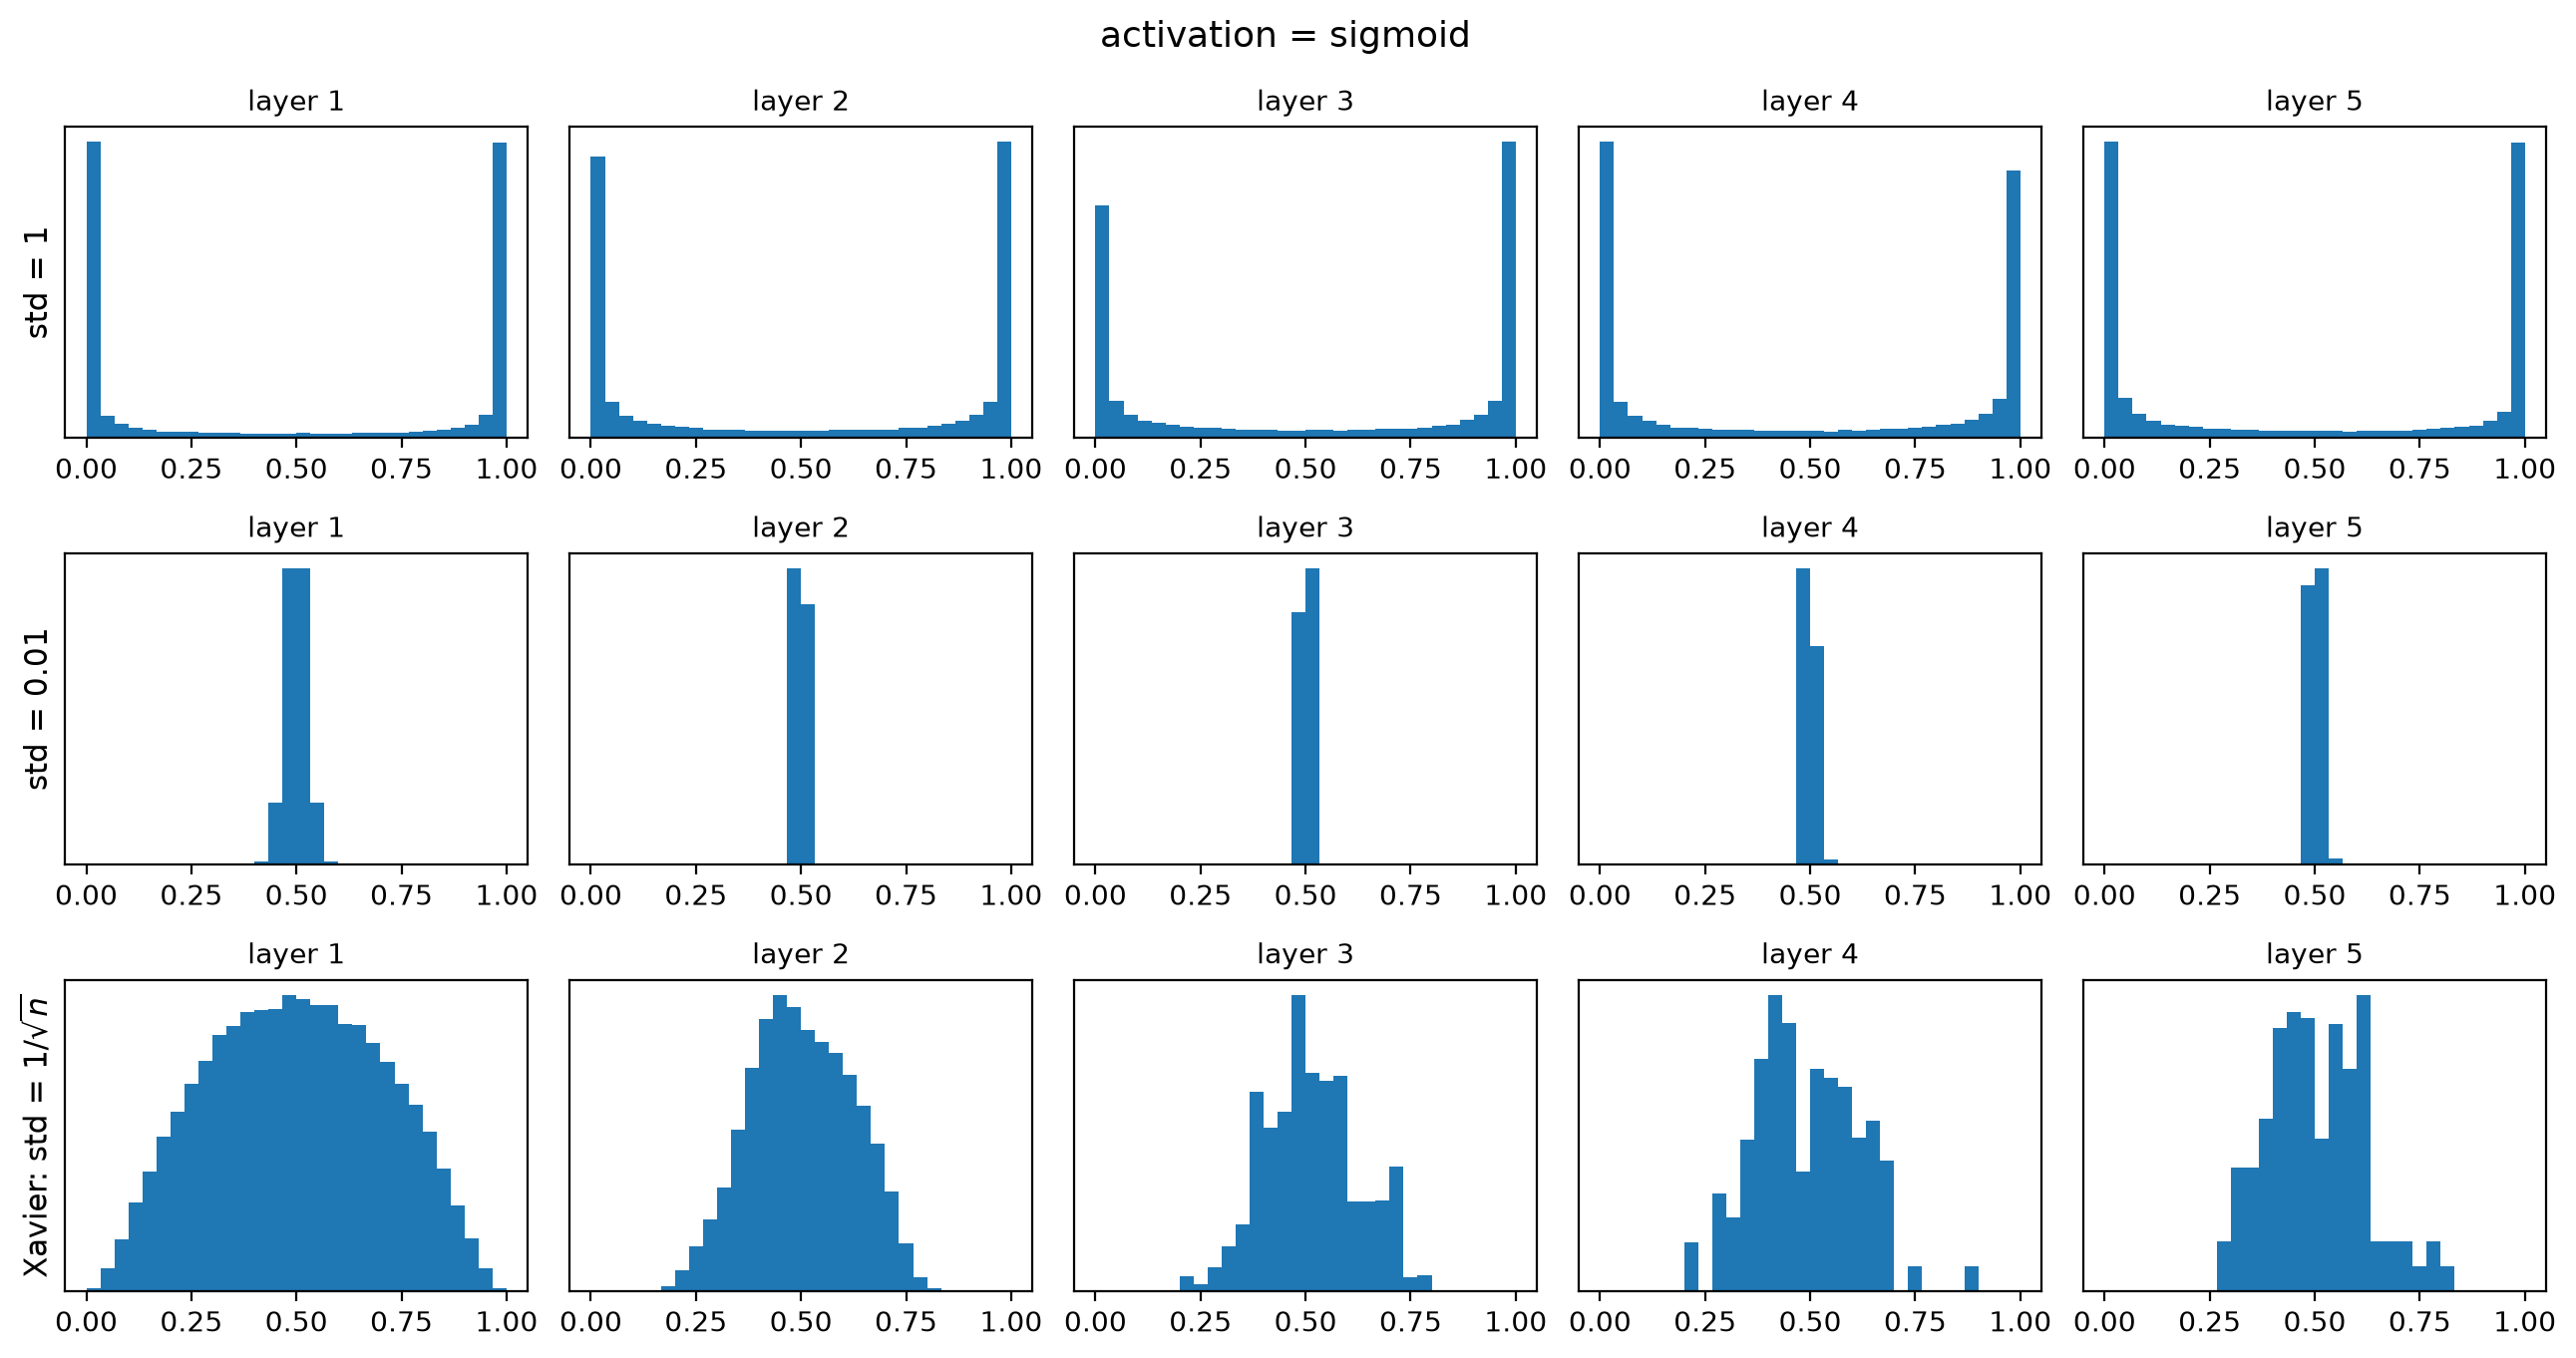
\includegraphics[height=0.52\textheight]{init_sigmoid.png}
\raggedright
\small
\begin{itemize}
\item \code{std = 1}: $0$과 $1$에 몰린다 $\to$ sigmoid의 기울기 $\sigma(1-\sigma)\approx0$ $\to$ \textbf{기울기 소실}
\item \code{std = 0.01}: 모두 $0.5$ 근처 $\to$ 노드 100개가 거의 같은 값 $\to$ 노드가 많아도 \textbf{하나나 다름없다}
\item Xavier: 넓게 퍼진다
\end{itemize}
\end{frame}

\begin{frame}{그림: tanh와 ReLU (\code{init\_tanh.png}, \code{init\_relu.png})}
\begin{columns}[T,onlytextwidth]
\begin{column}{0.49\textwidth}
\centering
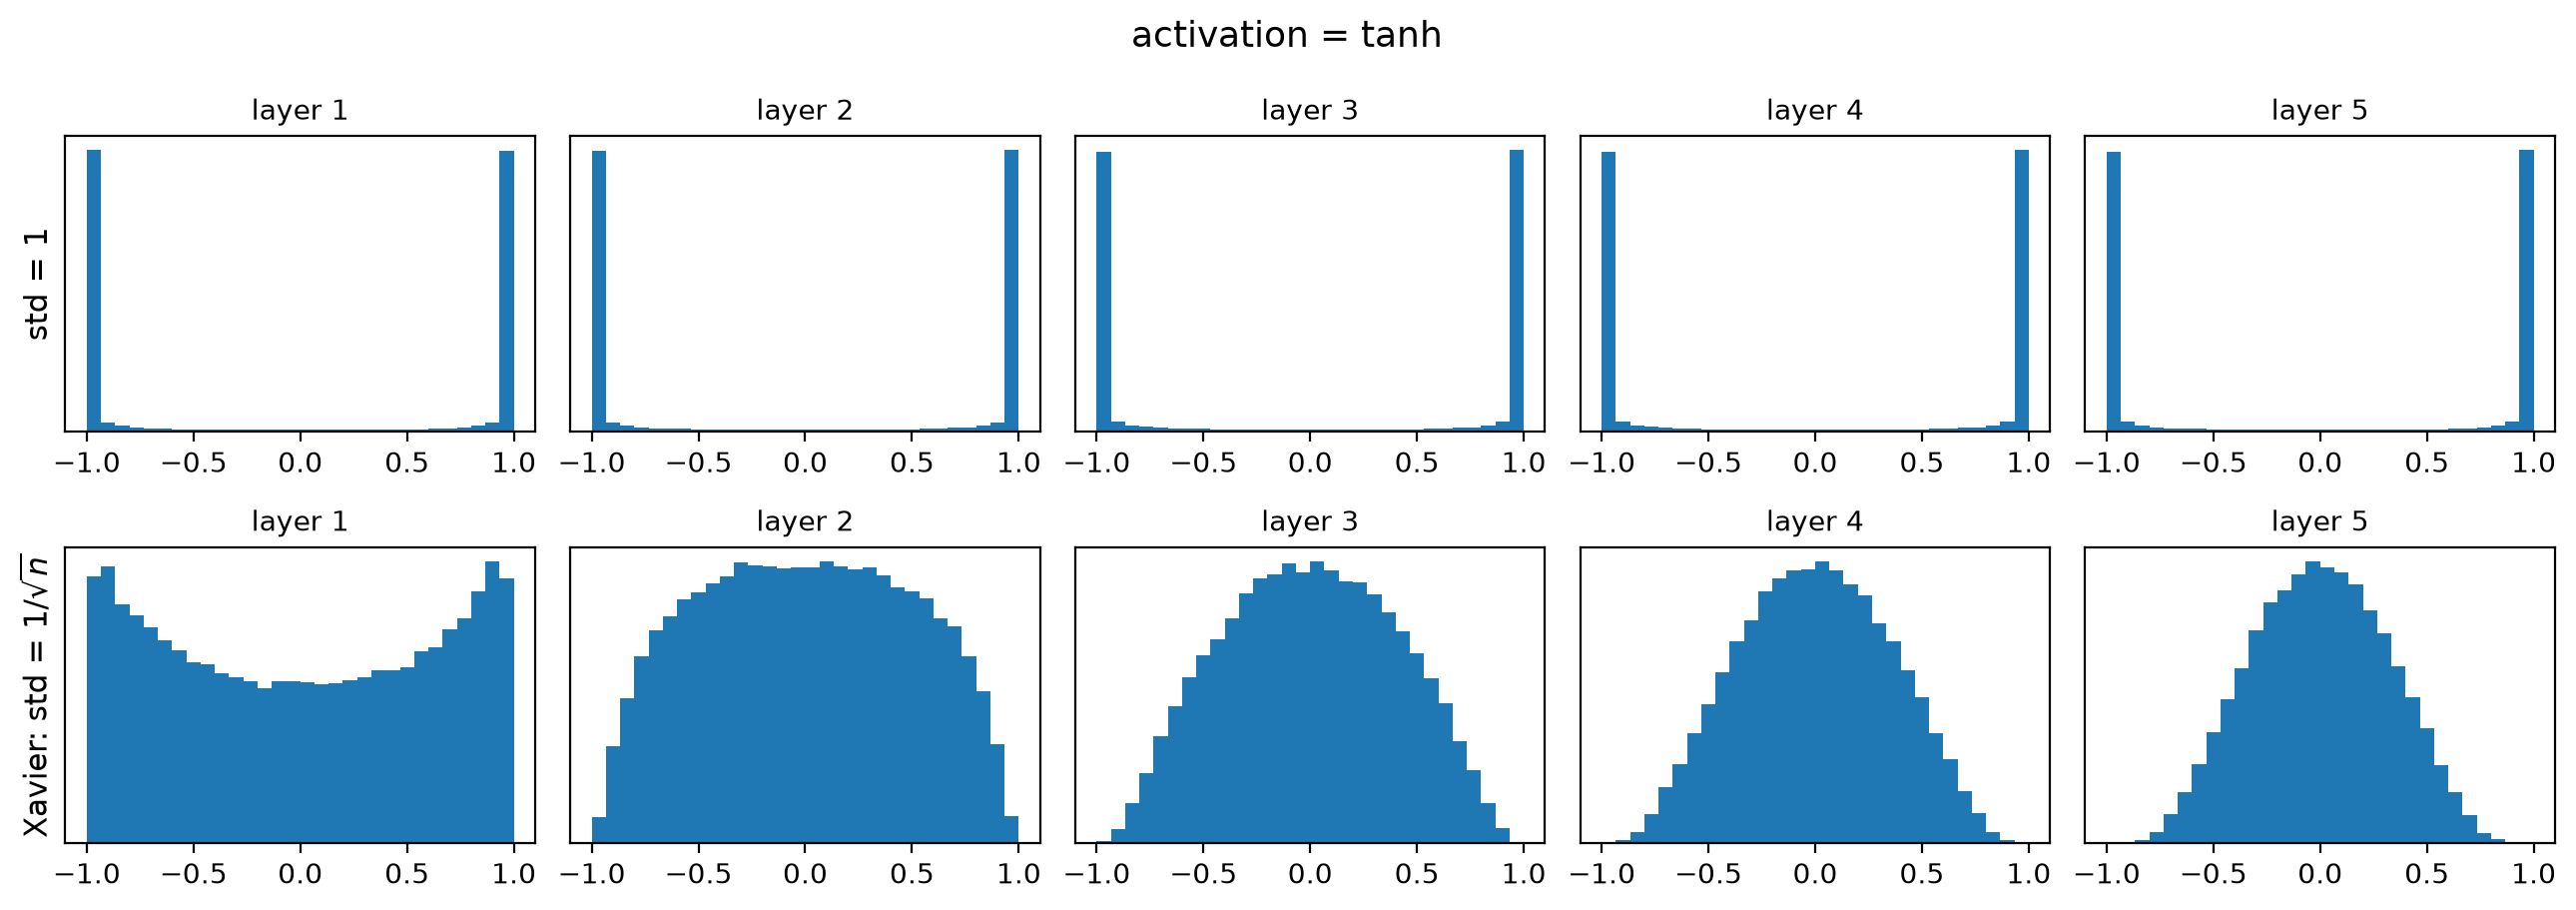
\includegraphics[width=\linewidth]{init_tanh.png}
\raggedright
\footnotesize
\begin{itemize}
\item \code{std = 1}: $\pm1$에 몰림 (포화)
\item Xavier: $0$을 중심으로 고르게. 다만 층이 깊어질수록 조금씩 좁아진다
\end{itemize}
\end{column}
\begin{column}{0.49\textwidth}
\centering
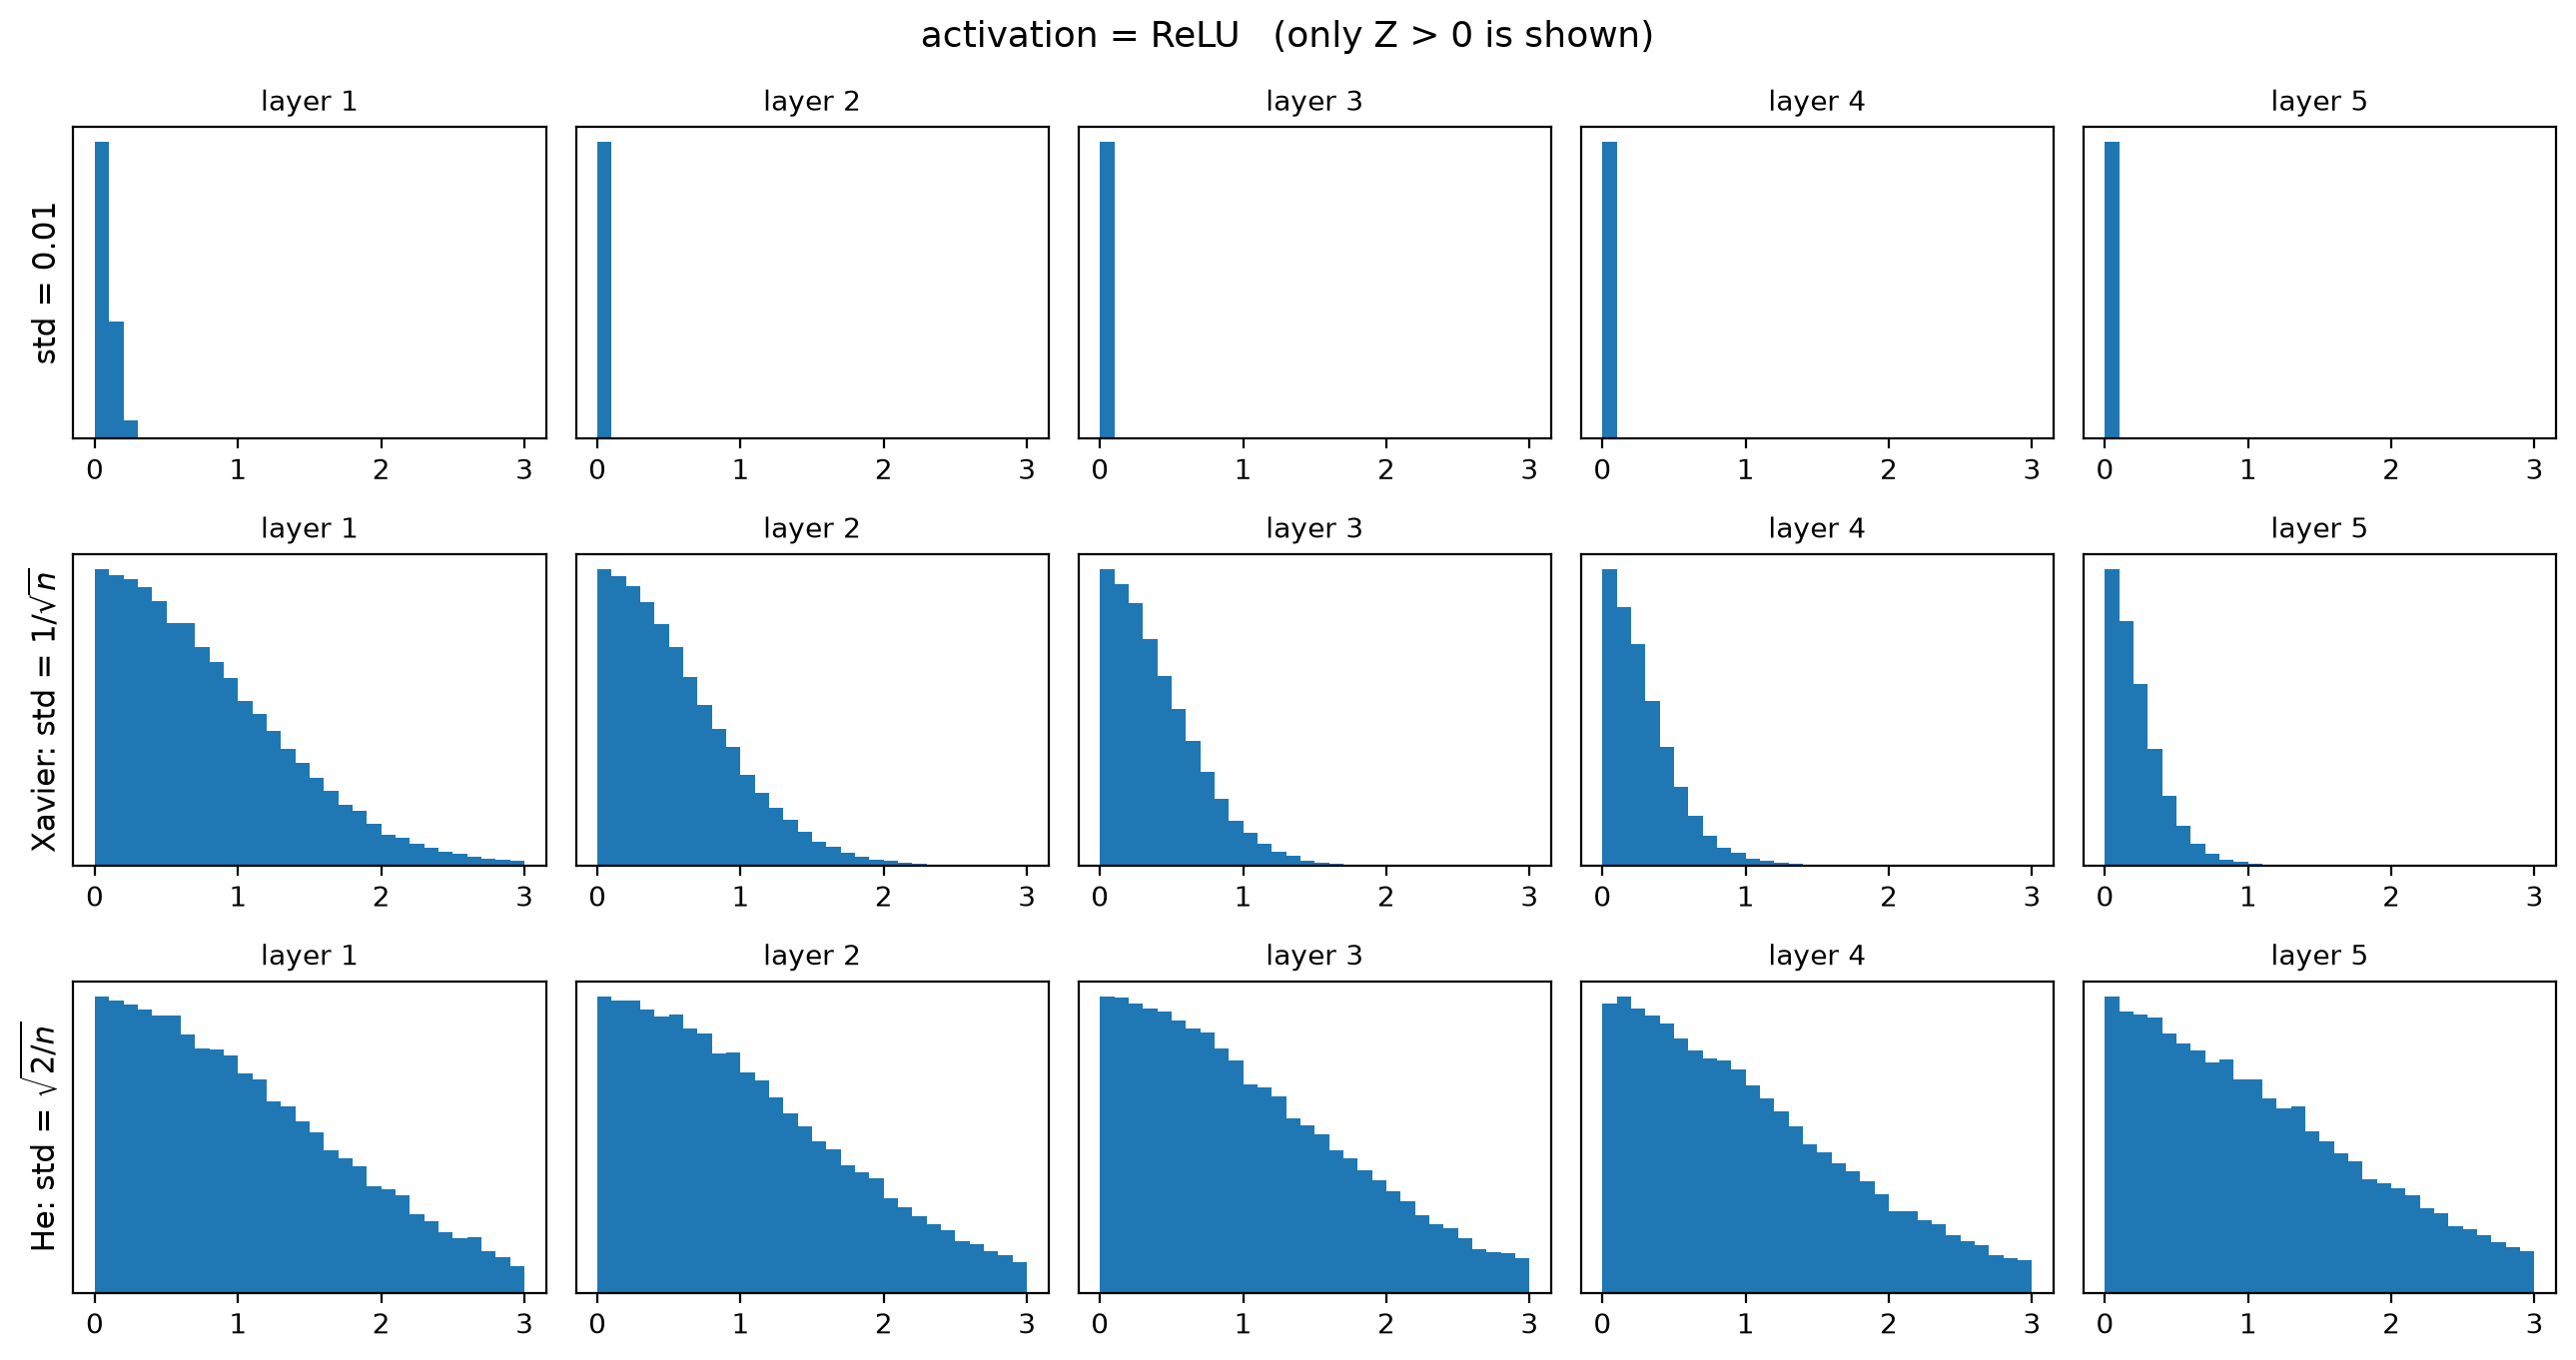
\includegraphics[width=\linewidth]{init_relu.png}
\raggedright
\footnotesize
\begin{itemize}
\item $Z>0$인 값만 그렸다
\item \code{std = 0.01}: 모두 $0$ 근처로 사라진다
\item Xavier: 층마다 좁아진다
\item He: 5층까지 \textbf{같은 모양}을 유지한다
\end{itemize}
\end{column}
\end{columns}
\end{frame}

% =================================================
\section{실험 2: \texttt{mnist\_optimizer\_compare.py}}
% =================================================

\begin{frame}[shrink,fragile]{설정: 같은 신경망, 갱신 규칙만 다르게}
\small
\begin{lstlisting}
from mnist_data import load_mnist_split
from layers import MultiLayerNet
from optimizers import SGD, Momentum, AdaGrad, Adam

x_train, t_train, x_val, t_val, x_test, t_test = load_mnist_split()

optimizers = {
    "SGD":      SGD(lr=0.01),
    "Momentum": Momentum(lr=0.01, beta=0.9),
    "AdaGrad":  AdaGrad(lr=0.01),
    "Adam":     Adam(lr=0.001),
}
hidden = [100, 100, 100, 100]      # 4 hidden layers, 100 nodes each
epochs = 5
batch_size = 128

N = x_train.shape[0]
iter_per_epoch = N // batch_size
\end{lstlisting}
\small
\begin{itemize}
\item 최적화 기법 객체 4개를 딕셔너리에. 학습률은 각 기법에서 흔히 쓰는 값
\item \code{MultiLayerNet}의 초기화는 기본값(표준편차 $0.05$), BatchNorm 없음. $55000 // 128 = 429$ iteration이 1 epoch
\end{itemize}
\end{frame}

\begin{frame}[shrink,fragile]{학습 루프: 바뀌는 줄은 하나}
\footnotesize
\begin{lstlisting}[basicstyle=\codetiny]
loss_hist = {}
val_hist = {}
for name, optimizer in optimizers.items():
    np.random.seed(1)                                   # the SAME initial weights for every optimizer
    net = MultiLayerNet(784, hidden, 10, activation="relu", loss="ce")
    np.random.seed(2)                                   # the SAME mini-batches for every optimizer
    loss_hist[name], val_hist[name] = [], []
    t0 = time.time()
    for epoch in range(epochs):
        perm = np.random.permutation(N)
        for it in range(iter_per_epoch):
            idx = perm[it * batch_size:(it + 1) * batch_size]
            loss = net.loss(x_train[idx], t_train[idx])
            grads = net.backward()
            optimizer.update(net.params, grads)         # <- the only line that differs
            loss_hist[name].append(loss)
        val_hist[name].append(net.accuracy(x_val, t_val))
        print(f"[{name:8s}] epoch {epoch + 1}: loss={loss:.4f}, "
              f"val acc={val_hist[name][-1]:.4f} ({time.time() - t0:.0f}s)")
\end{lstlisting}
\small
\begin{itemize}
\item 기법마다 신경망을 \textbf{새로} 만든다 (\code{seed(1)} 덕분에 초기 가중치는 같다). 미니배치 순서도 \code{seed(2)}로 같다
\item \code{loss\_hist[name]}: 미니배치마다의 손실 $5\times429=2145$개. \code{val\_hist[name]}: epoch마다 검증 정확도
\end{itemize}
\end{frame}

\begin{frame}[fragile]{그래프: 이동평균과 로그 축}
\begin{lstlisting}[basicstyle=\codesmall]
def smooth(y, w=50):
    """moving average over w iterations (the mini-batch loss is noisy)"""
    y = np.asarray(y)
    return np.convolve(y, np.ones(w) / w, mode="valid")

fig, ax = plt.subplots(1, 2, figsize=(12, 4.2))
for name in optimizers:
    ax[0].plot(smooth(loss_hist[name]), label=name)
ax[0].set_yscale("log")
...
for name in optimizers:
    ax[1].plot(range(1, epochs + 1), val_hist[name], "o-", label=name)
\end{lstlisting}
\small
\begin{itemize}
\item 미니배치 손실은 들쭉날쭉하다 $\to$ 연속한 $50$개의 \textbf{평균}으로 매끄럽게
\item \code{np.convolve(y, np.ones(w) / w)}: 길이 $w$의 창을 밀며 $\frac1w$씩 곱해 더하기 $=$ 이동평균
\item \code{mode="valid"}: 창이 끝까지 들어가는 곳만 $\to$ 길이 $2145-50+1=2096$
\item \code{for name in optimizers}: 딕셔너리를 돌면 \textbf{키}(이름)가 나온다
\end{itemize}
\end{frame}

\begin{frame}[fragile]{결과: \code{mnist\_optimizers.png}}
\begin{columns}[T,onlytextwidth]
\begin{column}{0.58\textwidth}
\centering
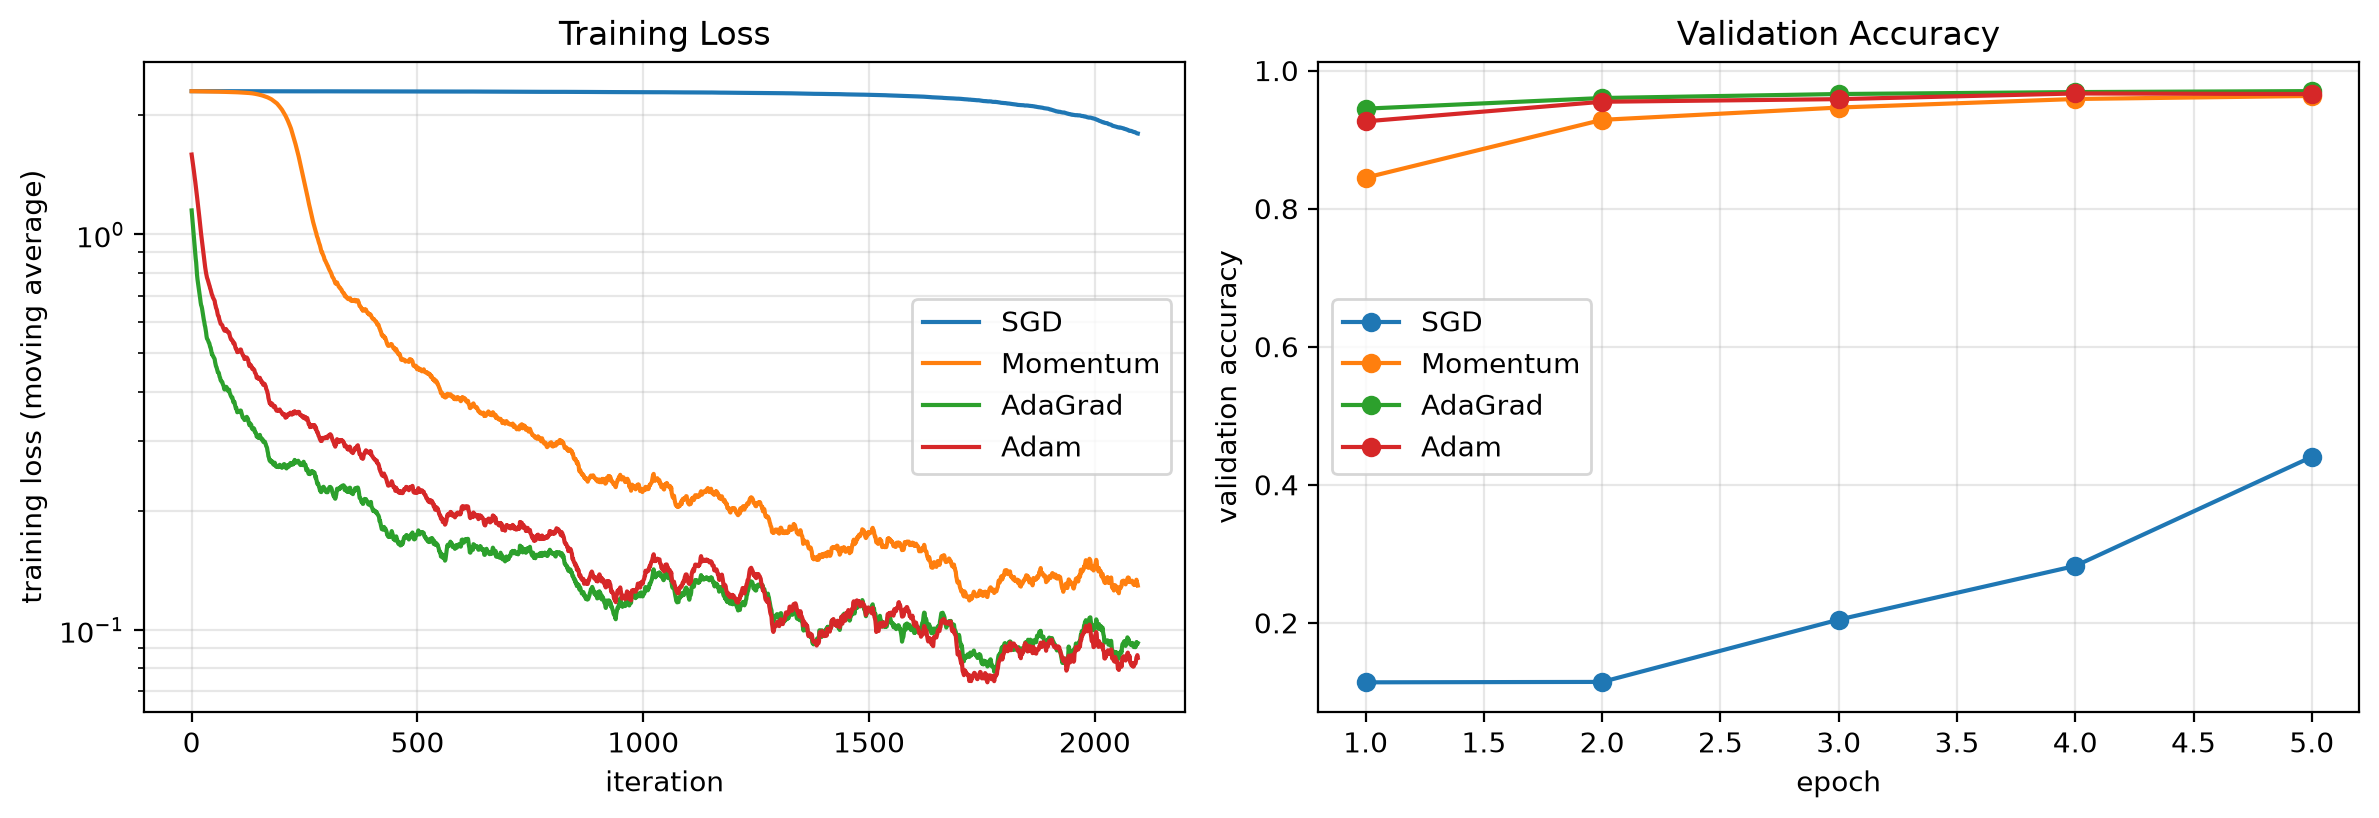
\includegraphics[width=\linewidth]{mnist_optimizers.png}
\end{column}
\begin{column}{0.38\textwidth}
\begin{lstlisting}[style=outstyle,basicstyle=\codesmall]
validation accuracy
after 5 epochs:
  SGD      0.4404
  Momentum 0.9632
  AdaGrad  0.9702
  Adam     0.9660
\end{lstlisting}
\end{column}
\end{columns}
\vskip2mm
\small
\begin{itemize}
\item SGD는 처음 약 1500 iteration 동안 손실이 거의 줄지 않는다 (검증 정확도 $11\%$: 찍는 것과 같다). 5 epoch 뒤에도 $44\%$
\item Momentum, AdaGrad, Adam은 첫 epoch부터 빠르게 내려간다. 이 설정에서는 AdaGrad가 조금 앞섰다
\item 결론: \textbf{같은 신경망이라도 갱신 규칙 하나로} 학습 속도가 크게 다르다
\end{itemize}
\end{frame}

% =================================================
\section{실험 3: \texttt{mnist\_init\_compare.py}}
% =================================================

\begin{frame}[shrink,fragile]{실험 2와 무엇이 다른가}
\footnotesize
\begin{lstlisting}[basicstyle=\codetiny]
inits = {
    "std = 0.01": 0.01,
    "Xavier":     "xavier",
    "He":         "he",
}
hidden = [100, 100, 100, 100, 100]      # 5 hidden layers, 100 nodes each
epochs = 5
batch_size = 128
learning_rate = 0.01

for name, init in inits.items():
    np.random.seed(1)
    net = MultiLayerNet(784, hidden, 10, activation="relu", loss="ce", weight_init_std=init)
    optimizer = SGD(lr=learning_rate)
    np.random.seed(2)                                   # the SAME mini-batches for every initialization
    ...   # the same training loop as mnist_optimizer_compare.py
\end{lstlisting}
\small
\begin{itemize}
\item 바꾸는 것: \code{weight\_init\_std} \textbf{하나}. 최적화 기법은 모두 SGD($0.01$)로 같다
\item \code{weight\_init\_std}에 숫자 \code{0.01}이나 문자열 \code{"xavier"}, \code{"he"}를 그대로 넘긴다
\item 은닉층은 5개 (실험 2보다 하나 많다). 학습 루프와 그래프 코드는 실험 2와 \textbf{같다}
\item \code{optimizer = SGD(...)}가 \textbf{반복문 안}에 있다: 상태가 없는 SGD라 상관없지만, Adam 같은 기법은 신경망마다 새로 만들어야 한다
\end{itemize}
\end{frame}

\begin{frame}[fragile]{결과: \code{mnist\_init.png}}
\begin{columns}[T,onlytextwidth]
\begin{column}{0.58\textwidth}
\centering
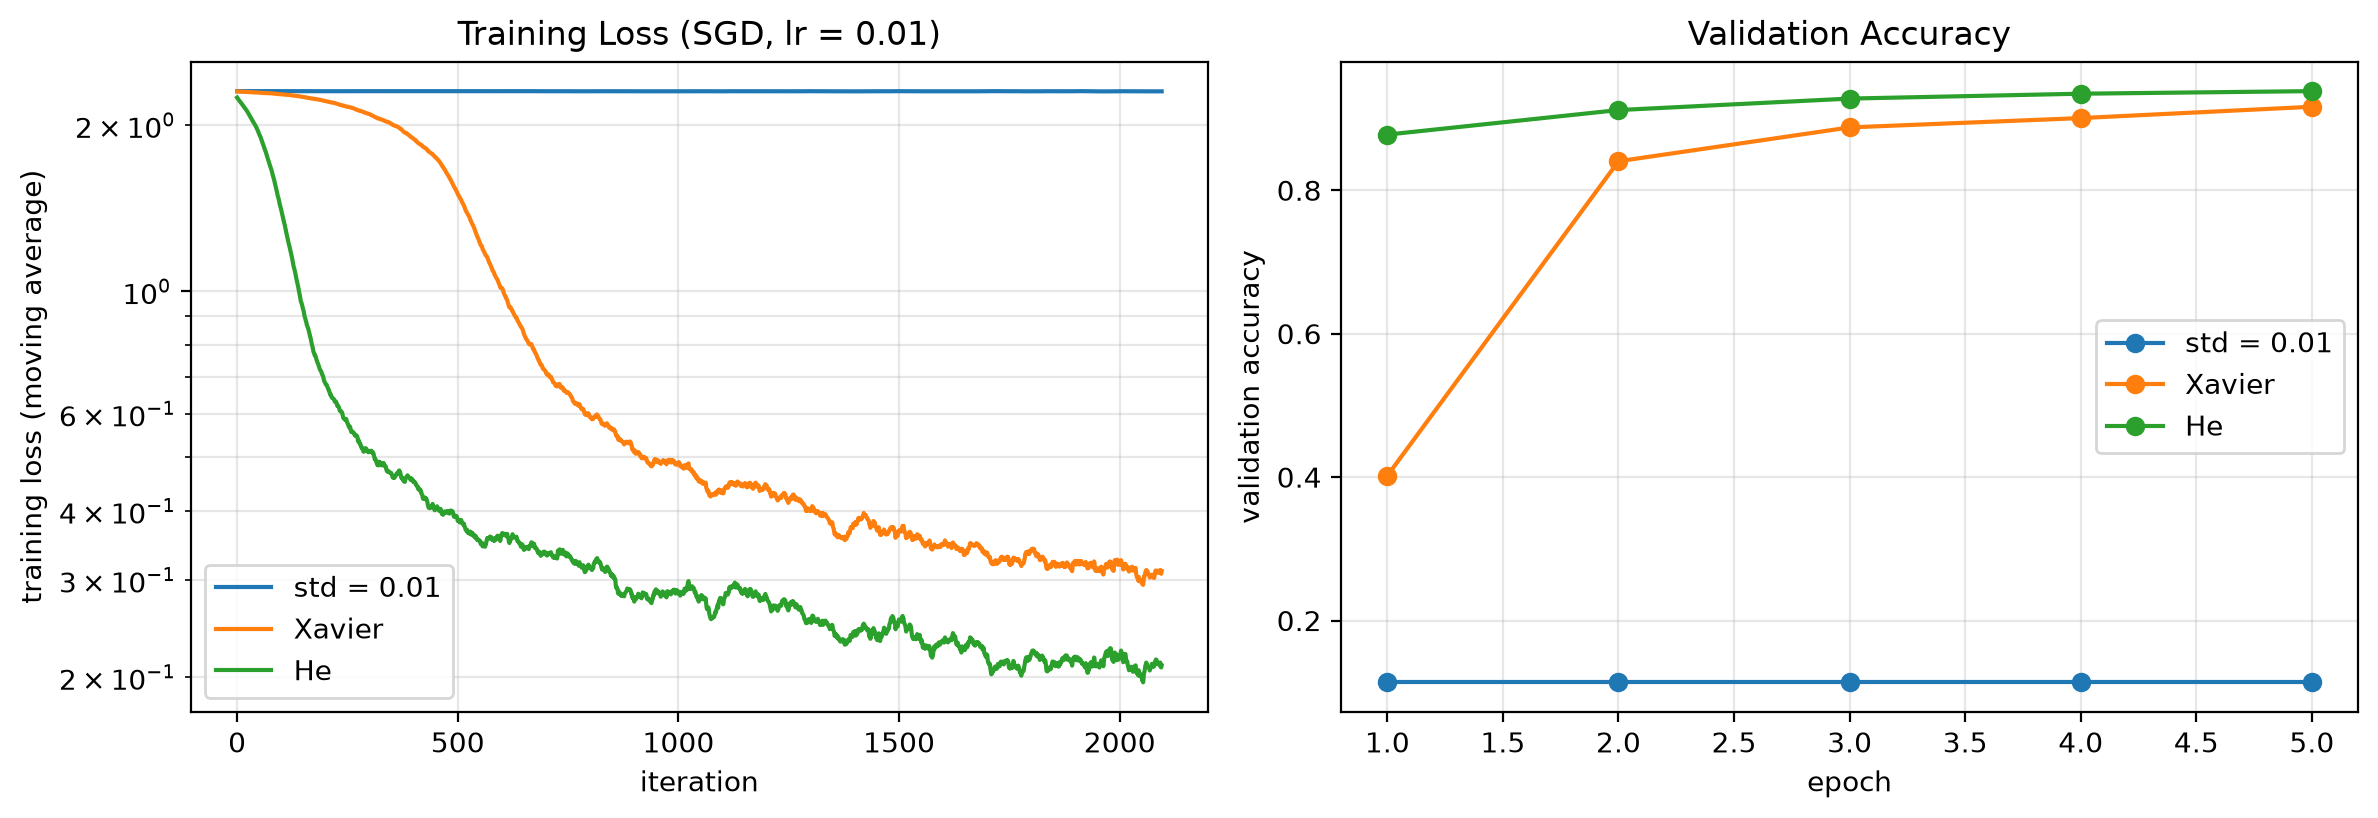
\includegraphics[width=\linewidth]{mnist_init.png}
\end{column}
\begin{column}{0.38\textwidth}
\begin{lstlisting}[style=outstyle,basicstyle=\codesmall]
validation accuracy
after 5 epochs:
  std = 0.01 0.1138
  Xavier     0.9164
  He         0.9382
\end{lstlisting}
\end{column}
\end{columns}
\vskip2mm
\small
\begin{itemize}
\item \code{std = 0.01}: 손실이 $2.30\approx\log10$에서 움직이지 않는다 (10개 중 찍기). 실험 1에서 본 것처럼 신호가 5층을 지나며 사라진다
\item He가 Xavier보다 빠르다: ReLU 신경망에서는 He가 신호의 크기를 유지하기 때문
\item 실험 1(분포)의 예측이 실제 학습(MNIST)에서도 그대로 나타났다
\end{itemize}
\end{frame}

% =================================================
\section{실험 4: \texttt{mnist\_batchnorm.py}}
% =================================================

\begin{frame}[shrink,fragile]{세 부분}
\small
\begin{enumerate}
\item \textbf{기울기 검사}: \code{BatchNormalization}의 역전파가 맞는지 수치 미분과 비교
\item \textbf{가중치 표준편차 16가지}: 훈련 이미지 $1000$장, BatchNorm이 있을 때와 없을 때
\item \textbf{MNIST 전체}: 실험 2의 신경망(SGD)에 BatchNorm만 더했을 때
\end{enumerate}
\begin{lstlisting}
def numerical_gradient(f, P, eps=1e-5):
    grad = np.zeros_like(P)
    for idx in np.ndindex(P.shape):
        old = P[idx]
        P[idx] = old + eps
        f_plus = f()
        P[idx] = old - eps
        f_minus = f()
        P[idx] = old
        grad[idx] = (f_plus - f_minus) / (2 * eps)
    return grad
\end{lstlisting}
\small
\begin{itemize}
\item 중심 차분 $\dfrac{f(p+\varepsilon)-f(p-\varepsilon)}{2\varepsilon}$을 \textbf{원소 하나씩}. \code{np.ndindex(P.shape)}: 모든 인덱스 \code{(i, j)}를 차례로
\item \code{f}: 인자 없는 함수. \code{P}를 제자리에서 바꾼 뒤 \code{f()}를 부르면 바뀐 값으로 손실이 계산된다
\end{itemize}
\end{frame}

\begin{frame}[fragile]{(1) 기울기 검사}
\begin{lstlisting}
np.random.seed(0)
small = MultiLayerNet(4, [5, 5], 3, weight_init_std=1.0, use_batchnorm=True)
X_small = np.random.randn(6, 4)
T_small = np.eye(3)[np.random.randint(0, 3, size=6)]
small.loss(X_small, T_small)
grads = small.backward()
for key in small.params:
    num = numerical_gradient(lambda: small.loss(X_small, T_small), small.params[key])
    print(f"{key:7s}: max |backprop - numerical| = {np.max(np.abs(grads[key] - num)):.2e}")
\end{lstlisting}
\begin{columns}[T,onlytextwidth]
\begin{column}{0.48\textwidth}
\begin{lstlisting}[style=outstyle,basicstyle=\codetiny]
W1     : max |backprop - numerical| = 2.48e-11
B1     : max |backprop - numerical| = 2.43e-17
gamma1 : max |backprop - numerical| = 2.48e-11
beta1  : max |backprop - numerical| = 1.64e-11
W2     : max |backprop - numerical| = 2.35e-11
B2     : max |backprop - numerical| = 1.11e-11
gamma2 : max |backprop - numerical| = 1.31e-11
beta2  : max |backprop - numerical| = 1.31e-11
W3     : max |backprop - numerical| = 2.85e-11
B3     : max |backprop - numerical| = 1.41e-11
\end{lstlisting}
\end{column}
\begin{column}{0.48\textwidth}
\footnotesize
\begin{itemize}
\item 작은 신경망 $4\to5\to5\to3$, 데이터 6개
\item \code{lambda: small.loss(...)}: 인자 없는 함수
\item 모든 매개변수에서 차이 $\approx10^{-11}$ $\to$ \textbf{역전파가 맞다}
\item \code{B1}만 $10^{-17}$: BatchNorm이 평균을 빼므로 $B_1$은 손실에 영향이 \textbf{없다} (기울기 $0$)
\end{itemize}
\end{column}
\end{columns}
\end{frame}

\begin{frame}[fragile]{공통 학습 함수 \code{train}}
\begin{lstlisting}
def train(net, X, T, epochs, batch_size, lr, X_eval, T_eval, seed=2):
    """plain SGD; return the mini-batch losses and the accuracy on (X_eval, T_eval) after each epoch"""
    optimizer = SGD(lr=lr)
    np.random.seed(seed)                          # the SAME mini-batches for every network
    N = X.shape[0]
    losses, accs = [], []
    for epoch in range(epochs):
        perm = np.random.permutation(N)
        for it in range(N // batch_size):
            idx = perm[it * batch_size:(it + 1) * batch_size]
            losses.append(net.loss(X[idx], T[idx]))
            optimizer.update(net.params, net.backward())
        accs.append(net.accuracy(X_eval, T_eval))
    return losses, accs
\end{lstlisting}
\small
\begin{itemize}
\item 실험 2, 3의 학습 루프를 \textbf{함수}로 묶었다. (2)와 (3)에서 여러 번 쓰기 위해
\item 학습 데이터 \code{(X, T)}와 평가 데이터 \code{(X\_eval, T\_eval)}를 인자로 받는다
\item \code{optimizer.update(net.params, net.backward())}: 두 줄을 한 줄로 썼다
\end{itemize}
\end{frame}

\begin{frame}[fragile]{(2) 가중치 표준편차 16가지}
\begin{lstlisting}[basicstyle=\codesmall]
x_small, t_small = x_train[:1000], t_train[:1000]
hidden = [100, 100, 100, 100, 100]               # 5 hidden layers, 100 nodes each
weight_scales = np.logspace(0, -4, num=16)       # 1, ..., 0.0001
epochs_small = 20

fig, axes = plt.subplots(4, 4, figsize=(13, 10))
for ax, w in zip(axes.ravel(), weight_scales):
    curves = {}
    for use_bn in (True, False):
        np.random.seed(1)                         # the SAME initial weights
        net = MultiLayerNet(784, hidden, 10, weight_init_std=w, use_batchnorm=use_bn)
        _, accs = train(net, x_small, t_small, epochs_small, 100, 0.01, x_small, t_small)
        curves[use_bn] = accs
    ax.plot(range(1, epochs_small + 1), curves[True], label="Batch Norm", color="tab:red")
    ax.plot(range(1, epochs_small + 1), curves[False], "--", label="without BN", color="tab:blue")
    ...
\end{lstlisting}
\small
\begin{itemize}
\item \code{np.logspace(0, -4, num=16)}: $10^0$부터 $10^{-4}$까지 \textbf{로그 간격}으로 16개 ($1, 0.54, 0.29, \ldots$)
\item \code{\_, accs = train(...)}: 손실은 버리고(\code{\_}) 정확도만. 평가도 같은 1000장(\textbf{훈련 정확도})
\item 16칸 $\times$ (BN 있음, 없음) $=$ 32번 학습. 이 컴퓨터에서 약 70초
\end{itemize}
\end{frame}

\begin{frame}[shrink,fragile]{(2) 결과: \code{bn\_weight\_scales.png}}
\small
\begin{columns}[T,onlytextwidth]
\begin{column}{0.52\textwidth}
\centering
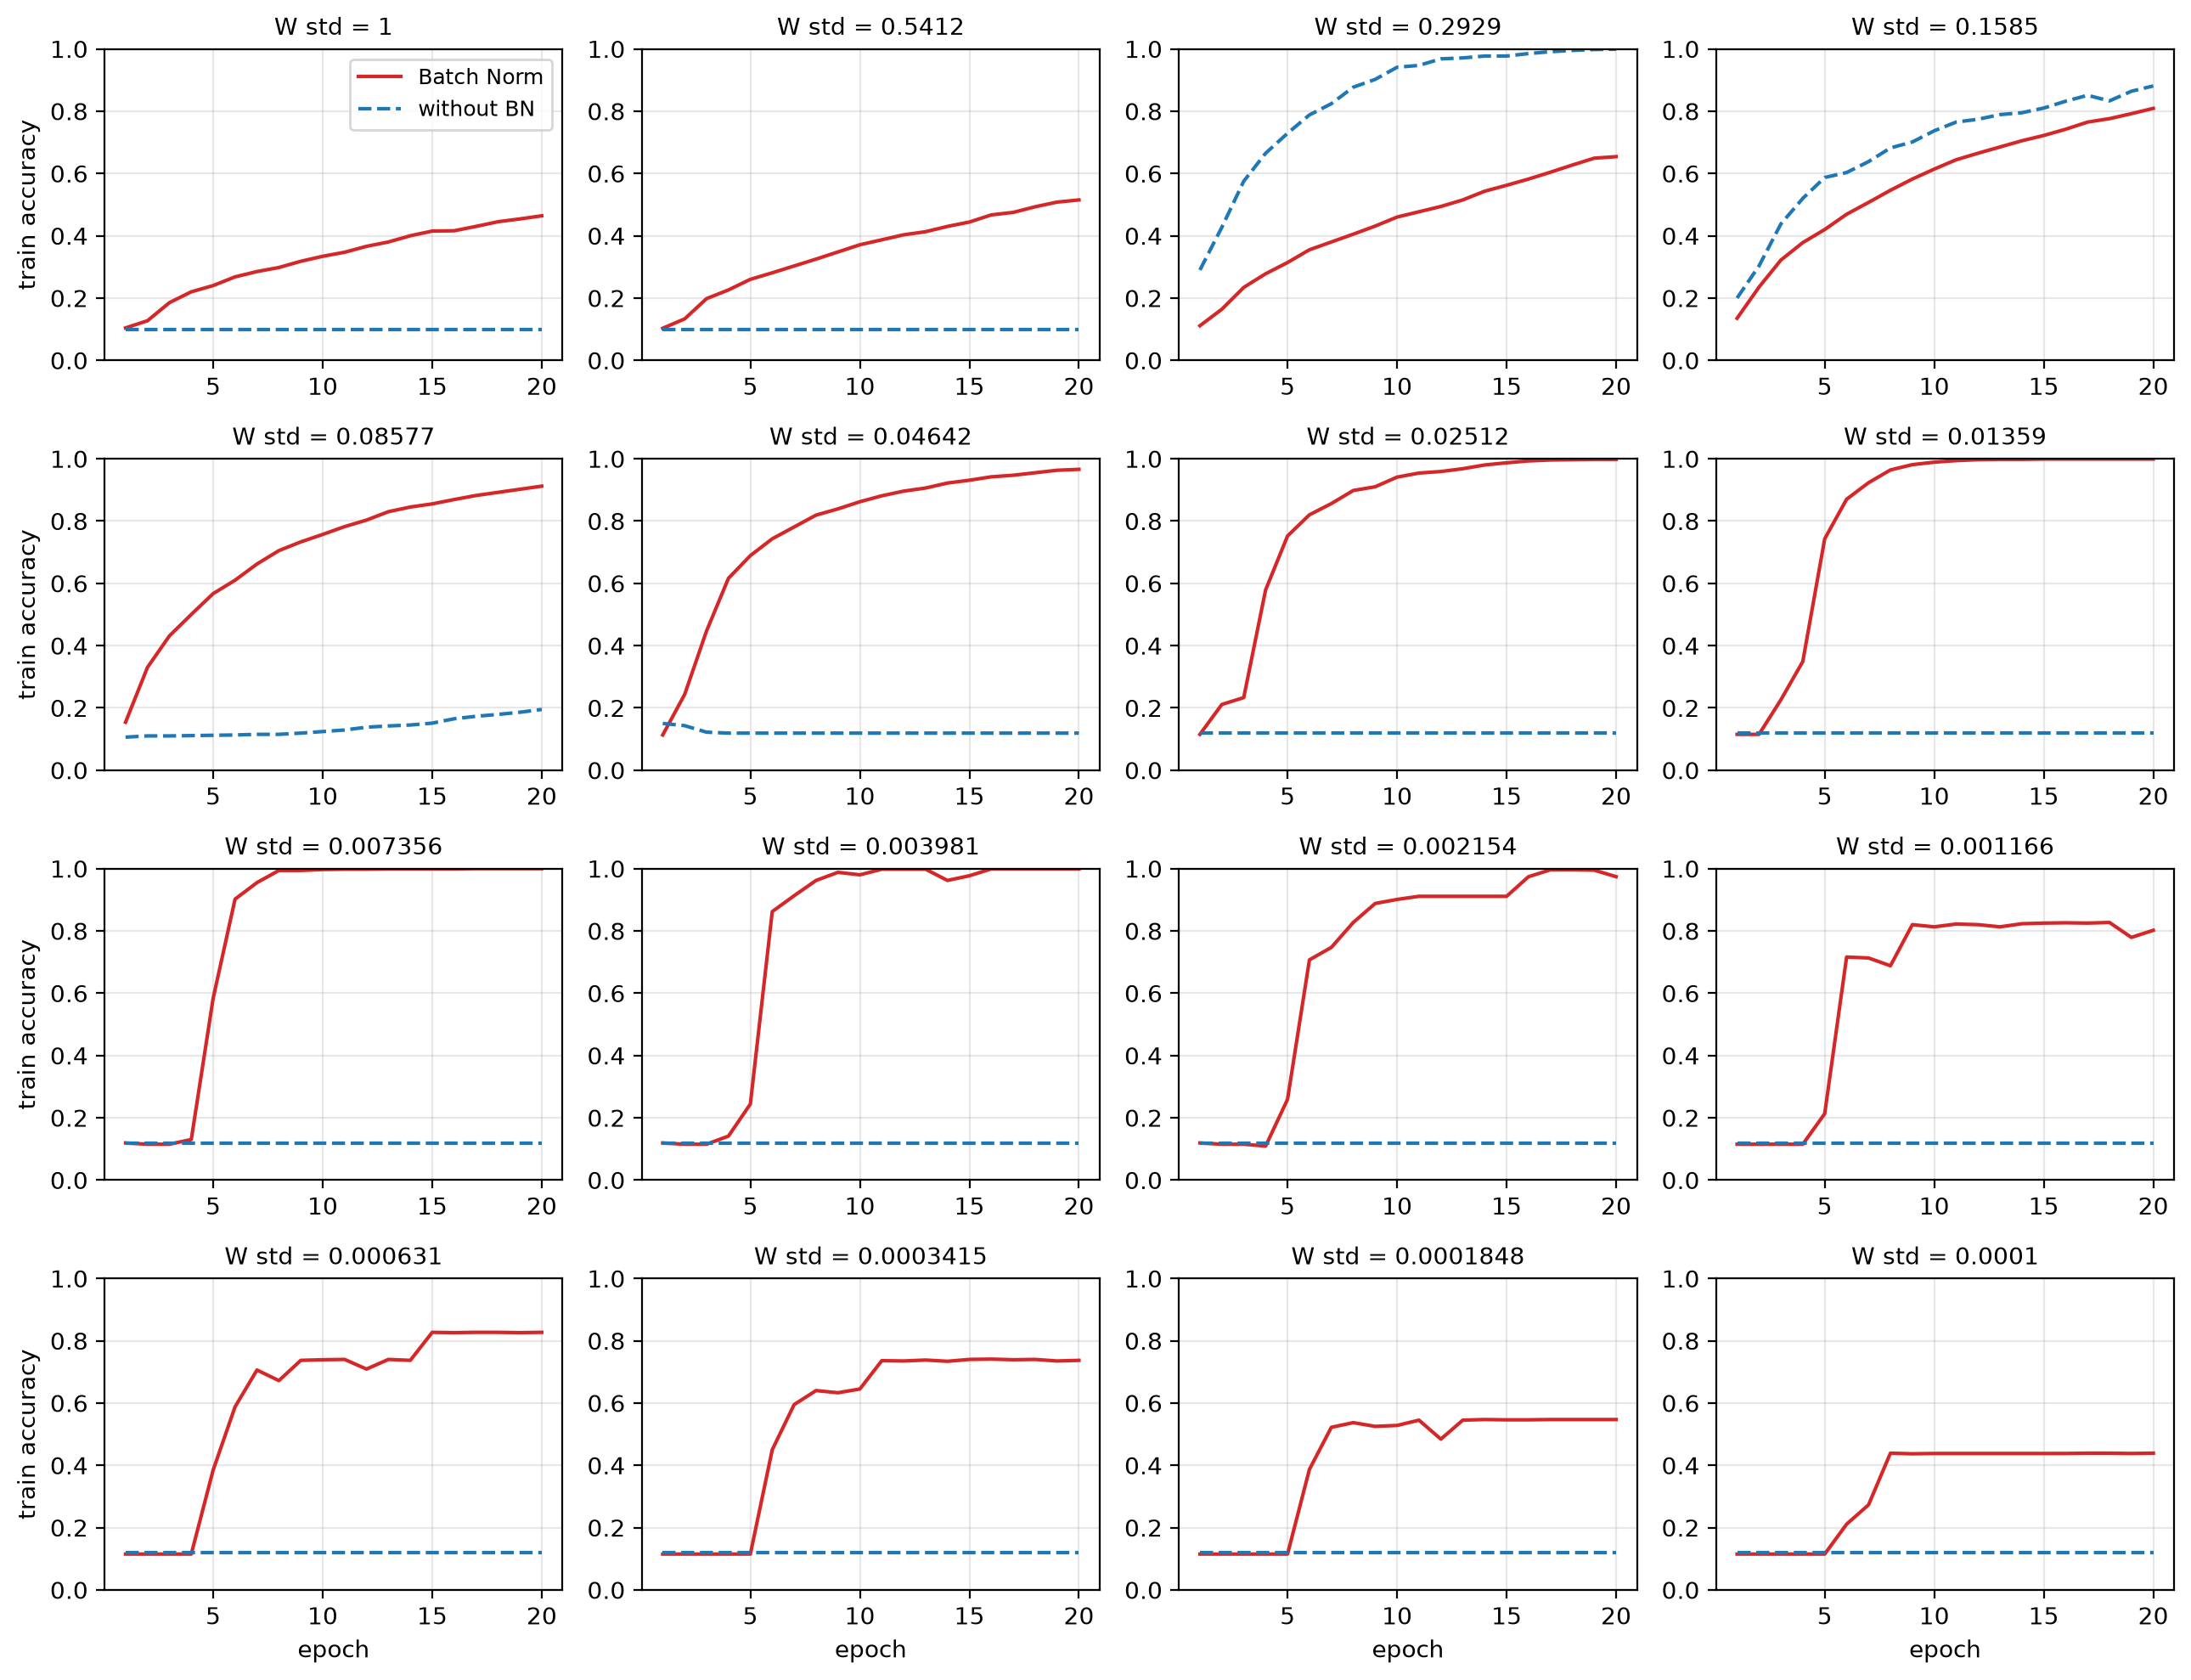
\includegraphics[width=\linewidth]{bn_weight_scales.png}
\end{column}
\begin{column}{0.44\textwidth}
\begin{lstlisting}[style=outstyle,basicstyle=\codetiny]
std 1:         BN=0.464  noBN=0.099
std 0.5412:    BN=0.515  noBN=0.099
std 0.2929:    BN=0.654  noBN=0.999
std 0.1585:    BN=0.809  noBN=0.881
std 0.08577:   BN=0.912  noBN=0.195
std 0.04642:   BN=0.966  noBN=0.119
std 0.02512:   BN=0.998  noBN=0.119
std 0.01359:   BN=0.999  noBN=0.119
std 0.007356:  BN=1.000  noBN=0.119
std 0.003981:  BN=0.999  noBN=0.119
std 0.002154:  BN=0.974  noBN=0.119
std 0.001166:  BN=0.802  noBN=0.119
...
std 0.0001:    BN=0.439  noBN=0.119
\end{lstlisting}
\footnotesize
(20 epoch 뒤 훈련 정확도. 출력을 줄여 옮겼다)
\end{column}
\end{columns}
\small
\begin{itemize}
\item BatchNorm 없이는 표준편차 $0.29$, $0.16$ \textbf{두 곳에서만} 학습된다. BatchNorm이 있으면 넓은 범위에서 학습된다
\item 표준편차 $1$, $0.54$ (BN 없음): 값이 넘쳐 \code{nan} (실행 중 \code{overflow} 경고) $\to$ 정확도 $0.099$
\end{itemize}
\end{frame}

\begin{frame}[fragile]{(3) MNIST 전체: \code{bn\_mnist.png}}
\begin{lstlisting}[basicstyle=\codesmall]
for use_bn in (False, True):
    np.random.seed(1)
    net = MultiLayerNet(784, [100, 100, 100, 100], 10, weight_init_std=0.05, use_batchnorm=use_bn)
    results[use_bn] = train(net, x_train, t_train, 5, 128, 0.01, x_val, t_val)
\end{lstlisting}
\begin{columns}[T,onlytextwidth]
\begin{column}{0.56\textwidth}
\centering
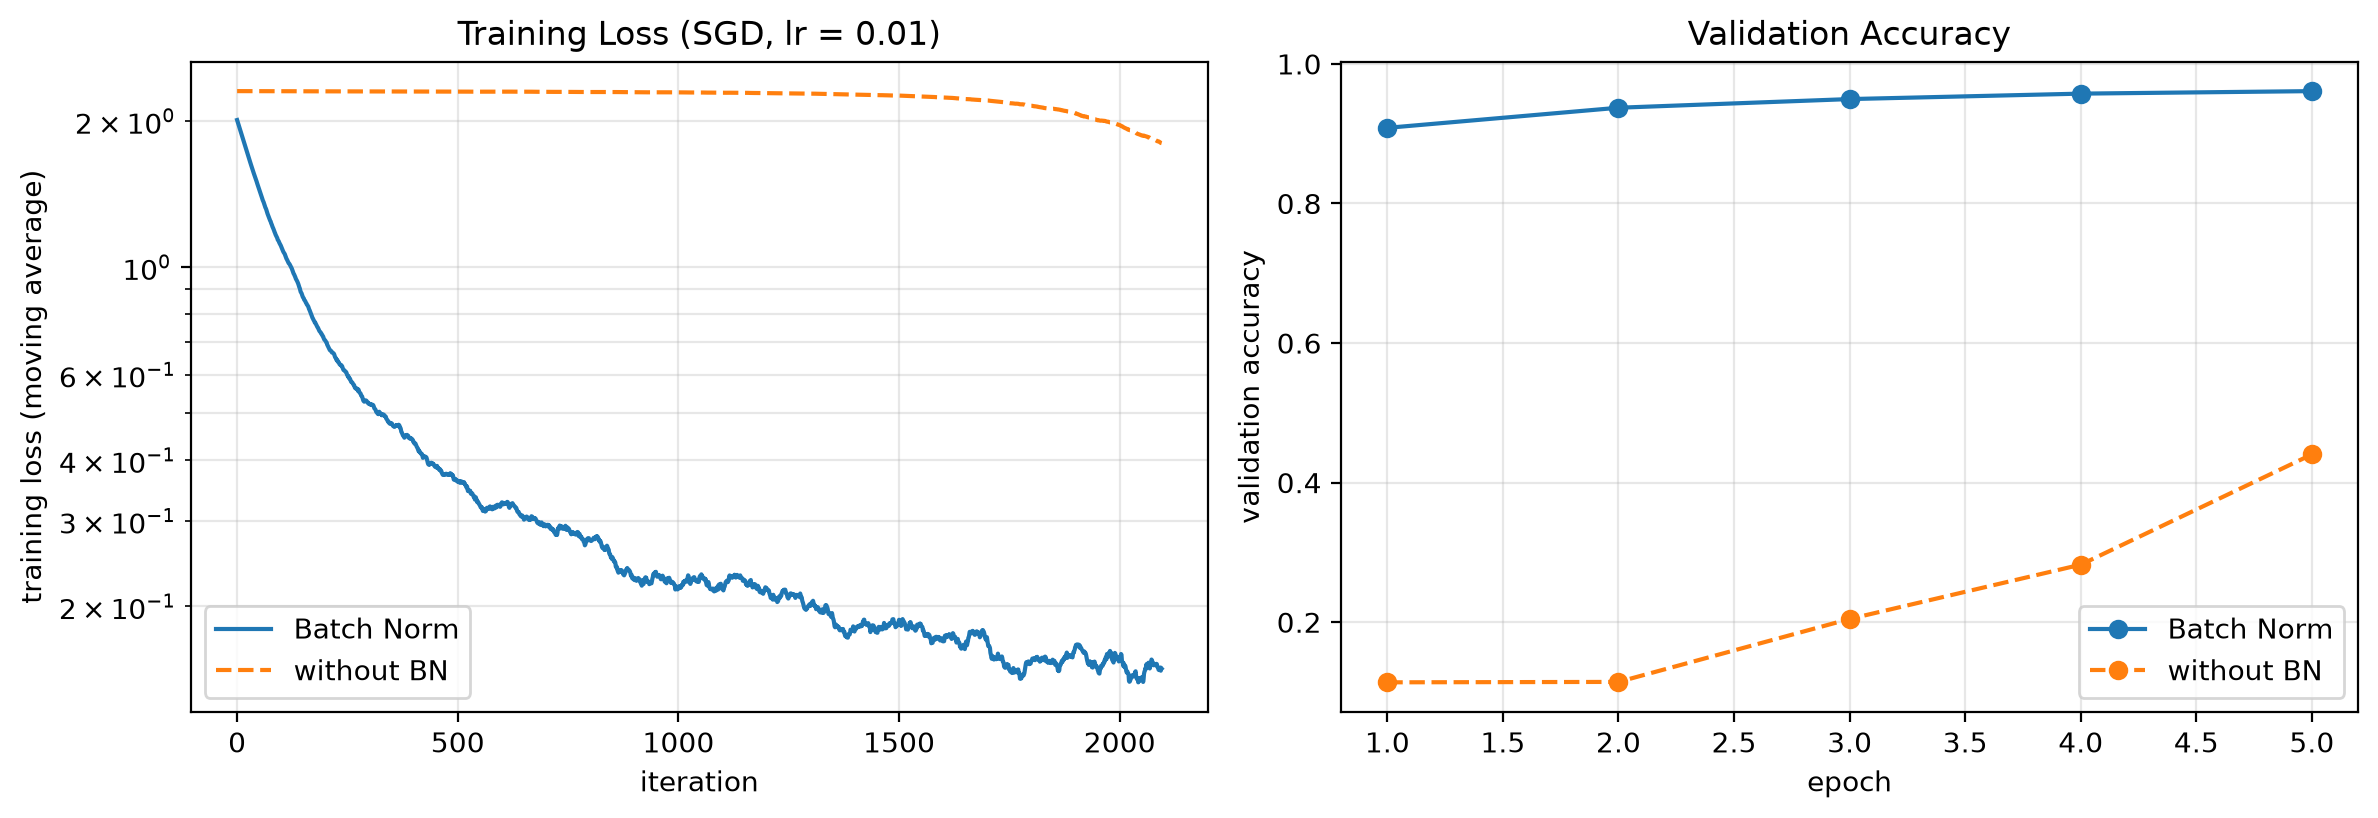
\includegraphics[width=\linewidth]{bn_mnist.png}
\end{column}
\begin{column}{0.40\textwidth}
\begin{lstlisting}[style=outstyle,basicstyle=\codetiny]
batch norm = False: val acc per epoch
  0.1138 0.1144 0.2046 0.2824 0.4404
batch norm = True: val acc per epoch
  0.9084 0.9372 0.9496 0.9574 0.9610
\end{lstlisting}
\footnotesize
\begin{itemize}
\item 실험 2의 SGD와 \textbf{같은} 설정. BatchNorm이 없으면 실험 2의 SGD와 숫자가 \textbf{똑같다} ($0.4404$)
\item BatchNorm만 더하면 첫 epoch에 $90.8\%$
\end{itemize}
\end{column}
\end{columns}
\end{frame}

% =================================================
\section{실험 5: \texttt{mnist\_overfit.py}}
% =================================================

\begin{frame}[fragile]{무엇을 하는 코드인가: 일부러 오버피팅 만들기}
\begin{lstlisting}
x_train, t_train, x_val, t_val, x_test, t_test = load_mnist_split()
x_train, t_train = x_train[:300], t_train[:300]   # only 300 training images -> overfitting

hidden = [100, 100, 100, 100, 100, 100]           # 6 hidden layers (7 Affine layers)
epochs = 300
batch_size = 100
\end{lstlisting}
\begin{itemize}
\item 훈련 데이터를 \textbf{300장}만 쓰고, 매개변수가 약 $13$만 개($130010$)인 깊은 신경망을 $300$ epoch 학습한다
\item 매개변수에 비해 데이터가 너무 적다 $\to$ 훈련 데이터를 \textbf{외워 버린다}
\item 다섯 부분:
\begin{enumerate}
\item 규제 없음 \quad (2) 가중치 감소 $\lambda=0.1$ \quad (3) 드롭아웃 $0.2$
\item[(4)] $\lambda$의 크기를 \textbf{검증 데이터}로 고르기
\item[(5)] Adam, Adam + L2, AdamW 비교
\end{enumerate}
\item 이 실행은 $300$ epoch $\times$ 11번 학습이라 가장 오래 걸린다 (이 컴퓨터에서 약 9분)
\end{itemize}
\end{frame}

\begin{frame}[shrink,fragile]{세 개의 도우미 함수}
\footnotesize
\begin{lstlisting}[basicstyle=\codetiny]
def train(net, optimizer, seed=2):
    """return the train / test accuracy after each epoch"""
    np.random.seed(seed)                          # the SAME mini-batches (and dropout masks)
    N = x_train.shape[0]
    train_acc, test_acc = [], []
    for epoch in range(epochs):
        perm = np.random.permutation(N)
        for it in range(N // batch_size):
            idx = perm[it * batch_size:(it + 1) * batch_size]
            net.loss(x_train[idx], t_train[idx])
            optimizer.update(net.params, net.backward())
        train_acc.append(net.accuracy(x_train, t_train))
        test_acc.append(net.accuracy(x_test, t_test))
    return train_acc, test_acc


def make_net(**options):
    np.random.seed(1)                             # the SAME initial weights
    return MultiLayerNet(784, hidden, 10, weight_init_std="he", **options)
\end{lstlisting}
\small
\begin{itemize}
\item \code{train}: epoch마다 \textbf{훈련}과 \textbf{test} 정확도를 기록. test는 오버피팅을 \textbf{보여 주는 데만} 쓴다 (고르는 데는 쓰지 않는다)
\item \code{**options}: 이름 붙은 인자를 딕셔너리로 모아 받고, 그대로 \code{MultiLayerNet}에 넘긴다
\begin{itemize}
\item \code{make\_net(weight\_decay\_lambda=0.1)} $\to$ \code{MultiLayerNet(784, hidden, 10, weight\_init\_std="he", weight\_decay\_lambda=0.1)}
\end{itemize}
\end{itemize}
\end{frame}

\begin{frame}[fragile]{그림과 출력 함수, (1)--(3) 실행}
\begin{lstlisting}[basicstyle=\codesmall]
def plot(train_acc, test_acc, title, filename):
    fig, ax = plt.subplots(figsize=(6, 4))
    ax.plot(range(1, epochs + 1), train_acc, label="train")
    ax.plot(range(1, epochs + 1), test_acc, "--", label="test")
    ...

def report(name, train_acc, test_acc):
    print(f"{name:22s} train {train_acc[-1]:.4f}  test {test_acc[-1]:.4f}  "
          f"gap {train_acc[-1] - test_acc[-1]:.4f}")

acc = train(make_net(), SGD(lr=0.01))
plot(*acc, "No regularization", "overfit.png")
report("no regularization", *acc)

acc = train(make_net(weight_decay_lambda=0.1), SGD(lr=0.01))
...
acc = train(make_net(use_dropout=True, dropout_ratio=0.2), SGD(lr=0.01))
\end{lstlisting}
\small
\begin{itemize}
\item \code{train}은 \code{(train\_acc, test\_acc)} 두 개를 튜플로 돌려준다 $\to$ \code{acc}
\item \code{plot(*acc, ...)}: 튜플을 \textbf{풀어서} 앞의 두 인자로. \code{plot(acc[0], acc[1], ...)}과 같다
\end{itemize}
\end{frame}

\begin{frame}[shrink,fragile]{(1)--(3) 결과}
\small
\begin{columns}[T,onlytextwidth]
\begin{column}{0.32\textwidth}
\centering
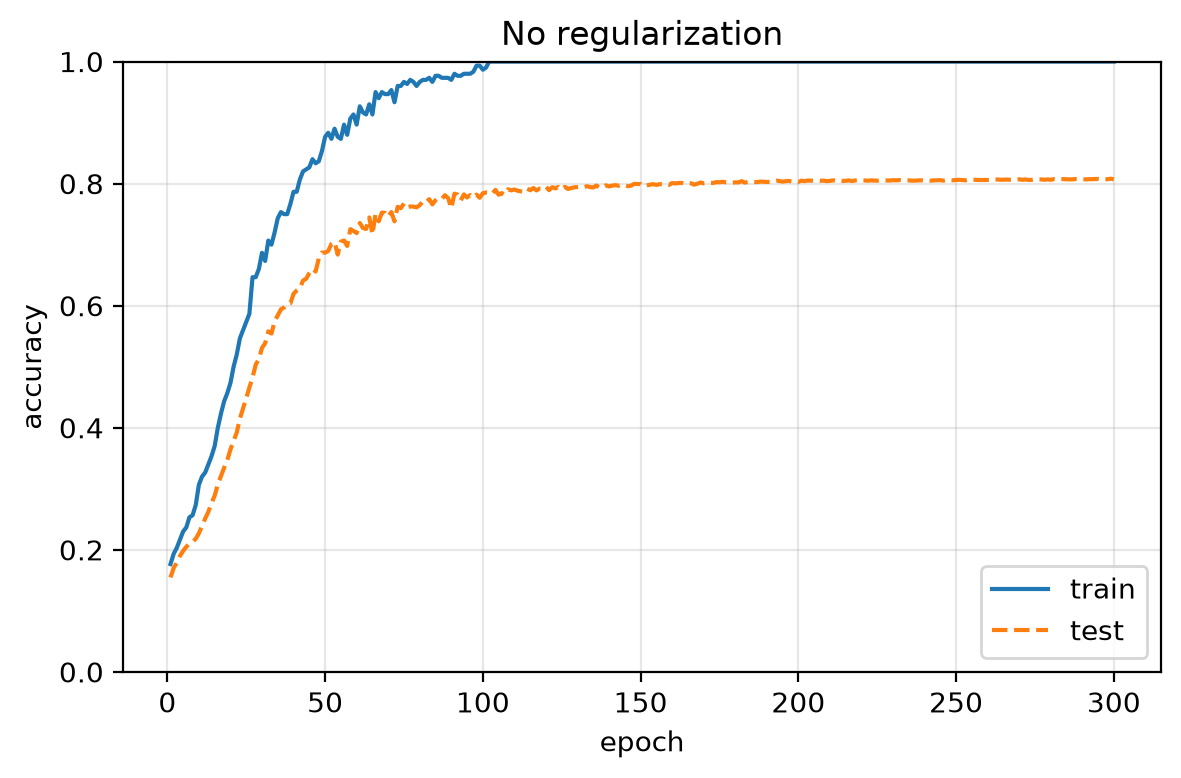
\includegraphics[width=\linewidth]{overfit.png}
\end{column}
\begin{column}{0.32\textwidth}
\centering
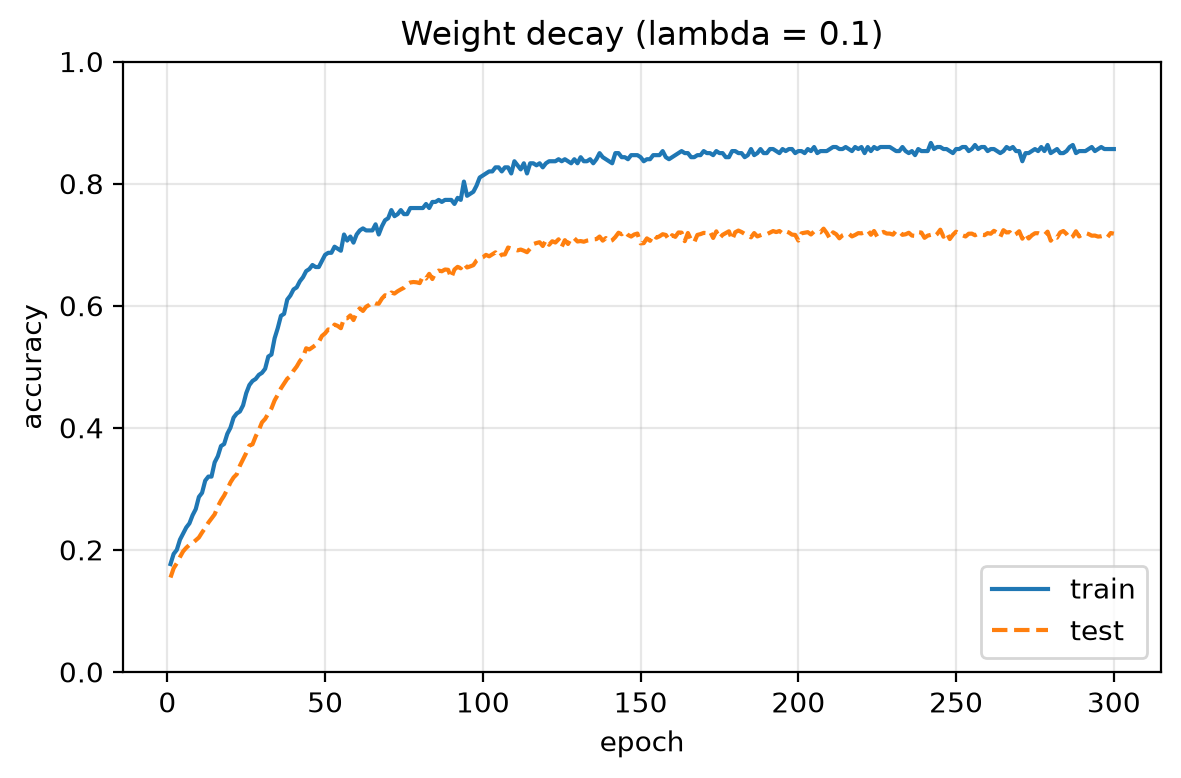
\includegraphics[width=\linewidth]{overfit_weight_decay.png}
\end{column}
\begin{column}{0.32\textwidth}
\centering
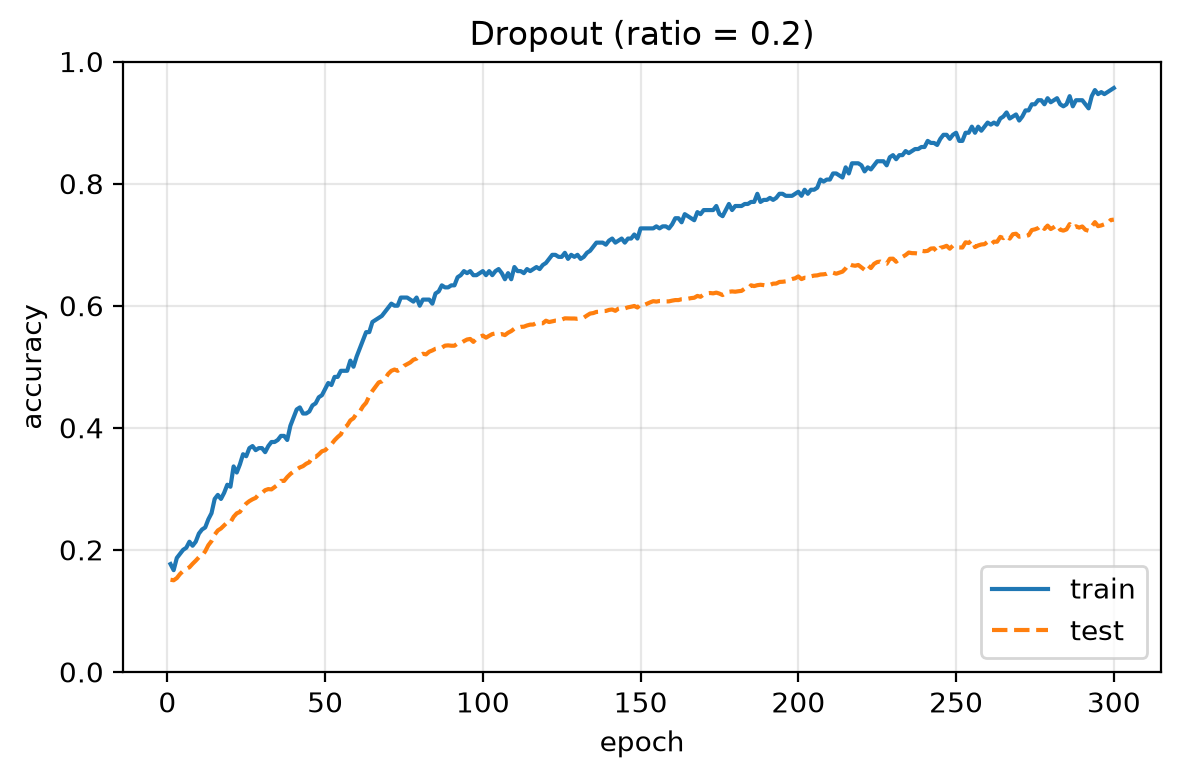
\includegraphics[width=\linewidth]{overfit_dropout.png}
\end{column}
\end{columns}
\begin{lstlisting}[style=outstyle,basicstyle=\codesmall]
no regularization      train 1.0000  test 0.8072  gap 0.1928
weight decay 0.1       train 0.8567  test 0.7180  gap 0.1387
dropout 0.2            train 0.9567  test 0.7410  gap 0.2157
\end{lstlisting}
\small
\begin{itemize}
\item 규제 없음: 약 $100$ epoch에 훈련 정확도 $100\%$, test는 $80.7\%$에서 멈춘다. 차이 $19.3\%$p가 오버피팅의 정도
\item 가중치 감소: 차이는 $13.9\%$p로 줄었지만 test도 $71.8\%$로 내려갔다 $\to$ $\lambda=0.1$은 \textbf{너무 강하다}
\item 드롭아웃: 훈련 정확도가 천천히 오른다(외우기 어렵다). 300 epoch에서 test는 아직 오르는 중이다
\end{itemize}
\end{frame}

\begin{frame}[fragile]{(4) $\lambda$는 검증 데이터로 고른다}
\begin{lstlisting}
for lam in (0.0, 0.01, 0.03, 0.1, 0.3):
    net = make_net(weight_decay_lambda=lam)
    train_acc, _ = train(net, SGD(lr=0.01))
    print(f"lambda = {lam:<5}: train {train_acc[-1]:.4f}  validation {net.accuracy(x_val, t_val):.4f}")
\end{lstlisting}
\begin{lstlisting}[style=outstyle]
lambda = 0.0  : train 1.0000  validation 0.8028
lambda = 0.01 : train 1.0000  validation 0.8064
lambda = 0.03 : train 1.0000  validation 0.8086
lambda = 0.1  : train 0.8567  validation 0.7076
lambda = 0.3  : train 0.1200  validation 0.1138
\end{lstlisting}
\begin{itemize}
\item \code{\{lam:<5\}}: 5칸 폭, 왼쪽 정렬. \code{train\_acc, \_ = ...}: test 정확도는 버린다 (\textbf{고를 때 보지 않는다})
\item 학습이 끝난 신경망으로 검증 정확도를 계산 $\to$ $\lambda=0.03$이 가장 좋다 ($80.86\%$)
\item $\lambda=0.3$: 훈련 데이터조차 학습하지 못한다 $\to$ \textbf{과소적합}(underfitting)
\item 300장뿐이라 어떤 규제로도 큰 향상은 어렵다. 가장 확실한 해결책은 \textbf{데이터를 늘리는 것}
\end{itemize}
\end{frame}

\begin{frame}[fragile]{(5) Adam, Adam + L2, AdamW}
\begin{lstlisting}
runs = {
    "Adam":             (make_net(), Adam(lr=0.001)),
    "Adam + L2 (0.1)":  (make_net(weight_decay_lambda=0.1), Adam(lr=0.001)),
    "AdamW (wd = 0.1)": (make_net(), AdamW(lr=0.001, weight_decay=0.1)),
}
for name, (net, optimizer) in runs.items():
    report(name, *train(net, optimizer))
\end{lstlisting}
\begin{lstlisting}[style=outstyle]
Adam                   train 1.0000  test 0.8326  gap 0.1674
Adam + L2 (0.1)        train 0.9167  test 0.7290  gap 0.1877
AdamW (wd = 0.1)       train 1.0000  test 0.8312  gap 0.1688
\end{lstlisting}
\small
\begin{itemize}
\item 딕셔너리의 값이 (신경망, 최적화 기법) \textbf{튜플}. \code{for name, (net, optimizer) in ...}: 한 번에 풀어 받는다
\item \code{report(name, *train(...))}: \code{train}이 돌려준 튜플을 풀어서 \code{report}의 인자로
\item 같은 $0.1$인데 결과가 다르다: L2는 $\sqrt{\hat v}$로 나뉘며 기울기가 작은 가중치를 강하게 눌러 과소적합,
AdamW는 한 걸음에 $\eta\lambda=10^{-4}$씩 줄어 $900$번 갱신 동안 $(1-10^{-4})^{900}\approx0.91$배로 영향이 작다
\end{itemize}
\end{frame}

% =================================================
\section{실험 6: \texttt{hyperparameter\_search.py}}
% =================================================

\begin{frame}[fragile]{무엇을 하는 코드인가: 무작위 탐색}
\begin{lstlisting}
x_train, t_train, x_val, t_val, x_test, t_test = load_mnist_split()   # 55000 / 5000 / 10000
x_train, t_train = x_train[:500], t_train[:500]   # a small training set -> fast trials
np.seterr(over="ignore", invalid="ignore")        # a too-large learning rate may blow up

epochs = 50
batch_size = 100
\end{lstlisting}
\begin{itemize}
\item 학습률과 가중치 감소 $\lambda$를 무작위로 \textbf{100번} 골라 학습해 보고, 검증 정확도로 가장 좋은 것을 찾는다
\item 한 번 시도에 시간이 오래 걸리면 100번을 할 수 없다 $\to$ 훈련 데이터를 \textbf{500장}으로 줄여 빨리
\item \code{np.seterr(...)}: 학습률이 너무 크면 값이 넘쳐(\code{overflow}) 경고가 100번 쏟아진다 $\to$ 경고를 끈다
\item 검증 데이터는 5000장 그대로. test는 \textbf{맨 마지막에 한 번}
\end{itemize}
\end{frame}

\begin{frame}[shrink,fragile]{한 번의 시도: \code{train(lr, weight\_decay)}}
\small
\begin{lstlisting}[basicstyle=\codesmall]
def train(lr, weight_decay, seed=2):
    """train a 7-layer network with SGD; return the network and the train / validation accuracy per epoch"""
    np.random.seed(1)                             # the SAME initial weights for every trial
    net = MultiLayerNet(784, [100, 100, 100, 100, 100, 100], 10,
                        weight_init_std="he", weight_decay_lambda=weight_decay)
    optimizer = SGD(lr=lr)
    np.random.seed(seed)                          # the SAME mini-batches for every trial
    N = x_train.shape[0]
    train_acc, val_acc = [], []
    for epoch in range(epochs):
        perm = np.random.permutation(N)
        for it in range(N // batch_size):
            idx = perm[it * batch_size:(it + 1) * batch_size]
            net.loss(x_train[idx], t_train[idx])
            optimizer.update(net.params, net.backward())
        train_acc.append(net.accuracy(x_train, t_train))
        val_acc.append(net.accuracy(x_val, t_val))   # VALIDATION data, not test data
    return net, train_acc, val_acc
\end{lstlisting}
\small
\begin{itemize}
\item 하이퍼파라미터 두 개를 인자로 받아 \textbf{신경망과 기록}을 돌려준다. 신경망 구조, 초기 가중치, 미니배치 순서는 매번 같다
\item 이번에는 test가 아니라 \textbf{검증} 정확도를 기록한다 (이것으로 고를 것이므로)
\end{itemize}
\end{frame}

\begin{frame}[shrink,fragile]{로그 스케일로 무작위 뽑기}
\small
\begin{lstlisting}
n_trials = 100
rng = np.random.default_rng(0)                    # separate random numbers for the sampling
results = []
for trial in range(n_trials):
    lr = 10 ** rng.uniform(-5, 0)                 # 1e-5 ~ 1
    weight_decay = 10 ** rng.uniform(-6, -1)      # 1e-6 ~ 0.1
    _, train_acc, val_acc = train(lr, weight_decay)
    results.append({"lr": lr, "wd": weight_decay, "train": train_acc, "val": val_acc})
    print(f"trial {trial + 1:3d}: val acc {val_acc[-1]:.4f}  lr {lr:.2e}  weight decay {weight_decay:.2e}")
\end{lstlisting}
\begin{lstlisting}[style=outstyle,basicstyle=\codesmall]
trial   1: val acc 0.8266  lr 1.53e-02  weight decay 2.23e-05
trial   2: val acc 0.1420  lr 1.60e-05  weight decay 1.21e-06
trial   3: val acc 0.8672  lr 1.17e-01  weight decay 3.66e-02
...
\end{lstlisting}
\small
\begin{itemize}
\item \code{10 ** rng.uniform(-5, 0)}: 지수를 $[-5,0)$에서 균등하게 $\to$ $10^{-5}$--$1$에서 \textbf{자릿수마다 같은 확률}
\item 그냥 \code{uniform(1e-5, 1)}이면 거의 다 $0.1$--$1$에서 뽑힌다 (작은 값은 거의 나오지 않는다)
\item \code{default\_rng(0)}: 뽑기용 난수를 \textbf{따로}. \code{train} 안의 \code{np.random.seed}와 섞이지 않는다
\end{itemize}
\end{frame}

\begin{frame}[fragile]{정렬해서 상위 10개 보기}
\begin{lstlisting}
results.sort(key=lambda r: r["val"][-1], reverse=True)
for rank, r in enumerate(results[:10], 1):
    print(f"{rank:2d}. val acc {r['val'][-1]:.4f}  train acc {r['train'][-1]:.4f}  "
          f"lr {r['lr']:.2e}  weight decay {r['wd']:.2e}")
\end{lstlisting}
\begin{lstlisting}[style=outstyle,basicstyle=\codesmall]
 1. val acc 0.8714  train acc 1.0000  lr 1.74e-01  weight decay 5.34e-06
 2. val acc 0.8672  train acc 0.9680  lr 1.17e-01  weight decay 3.66e-02
 3. val acc 0.8638  train acc 0.9920  lr 2.82e-01  weight decay 1.29e-02
 4. val acc 0.8618  train acc 1.0000  lr 1.12e-01  weight decay 6.34e-04
 5. val acc 0.8614  train acc 1.0000  lr 1.94e-01  weight decay 1.47e-06
 ...
10. val acc 0.8580  train acc 1.0000  lr 1.23e-01  weight decay 1.36e-03
\end{lstlisting}
\small
\begin{itemize}
\item \code{sort(key=..., reverse=True)}: 마지막 epoch의 검증 정확도가 \textbf{큰 순서}로. \code{lambda r: ...}: 기준을 꺼내는 작은 함수
\item \code{enumerate(..., 1)}: 순위를 $1$부터. \code{results[:10]}: 앞의 10개
\item 상위 10개의 학습률이 모두 $0.11$--$0.28$. 가중치 감소는 $10^{-6}$부터 $0.04$까지 제각각
\end{itemize}
\end{frame}

\begin{frame}[fragile]{학습률 구간별로 묶어 보기}
\begin{lstlisting}
edges = [1e-5, 1e-3, 1e-2, 3e-2, 1e-1, 3e-1, 1.0]
for lo, hi in zip(edges[:-1], edges[1:]):
    accs = [r["val"][-1] for r in results if lo <= r["lr"] < hi]
    print(f"lr {lo:.0e} ~ {hi:.0e}: {len(accs):3d} trials  best {max(accs):.4f}  mean {np.mean(accs):.4f}")
\end{lstlisting}
\begin{lstlisting}[style=outstyle]
lr 1e-05 ~ 1e-03:  34 trials  best 0.2198  mean 0.1631
lr 1e-03 ~ 1e-02:  20 trials  best 0.7760  mean 0.4722
lr 1e-02 ~ 3e-02:  10 trials  best 0.8352  mean 0.8018
lr 3e-02 ~ 1e-01:   8 trials  best 0.8546  mean 0.8472
lr 1e-01 ~ 3e-01:  16 trials  best 0.8714  mean 0.7975
lr 3e-01 ~ 1e+00:  12 trials  best 0.7218  mean 0.2899
\end{lstlisting}
\small
\begin{itemize}
\item \code{zip(edges[:-1], edges[1:])}: 이웃한 두 값의 쌍 $(10^{-5},10^{-3}), (10^{-3},10^{-2}), \ldots$
\item 학습률 $<10^{-3}$: 50 epoch 동안 거의 학습되지 않는다. \ $>0.3$: 자주 \textbf{발산}한다
\item 최고점은 $0.1$--$0.3$, 평균이 가장 높은 곳은 $0.03$--$0.1$ (최고점 근처는 발산 위험과 가깝다)
\end{itemize}
\end{frame}

\begin{frame}{그림: 상위 20개의 학습 곡선 (\code{hyper\_top20.png})}
\centering
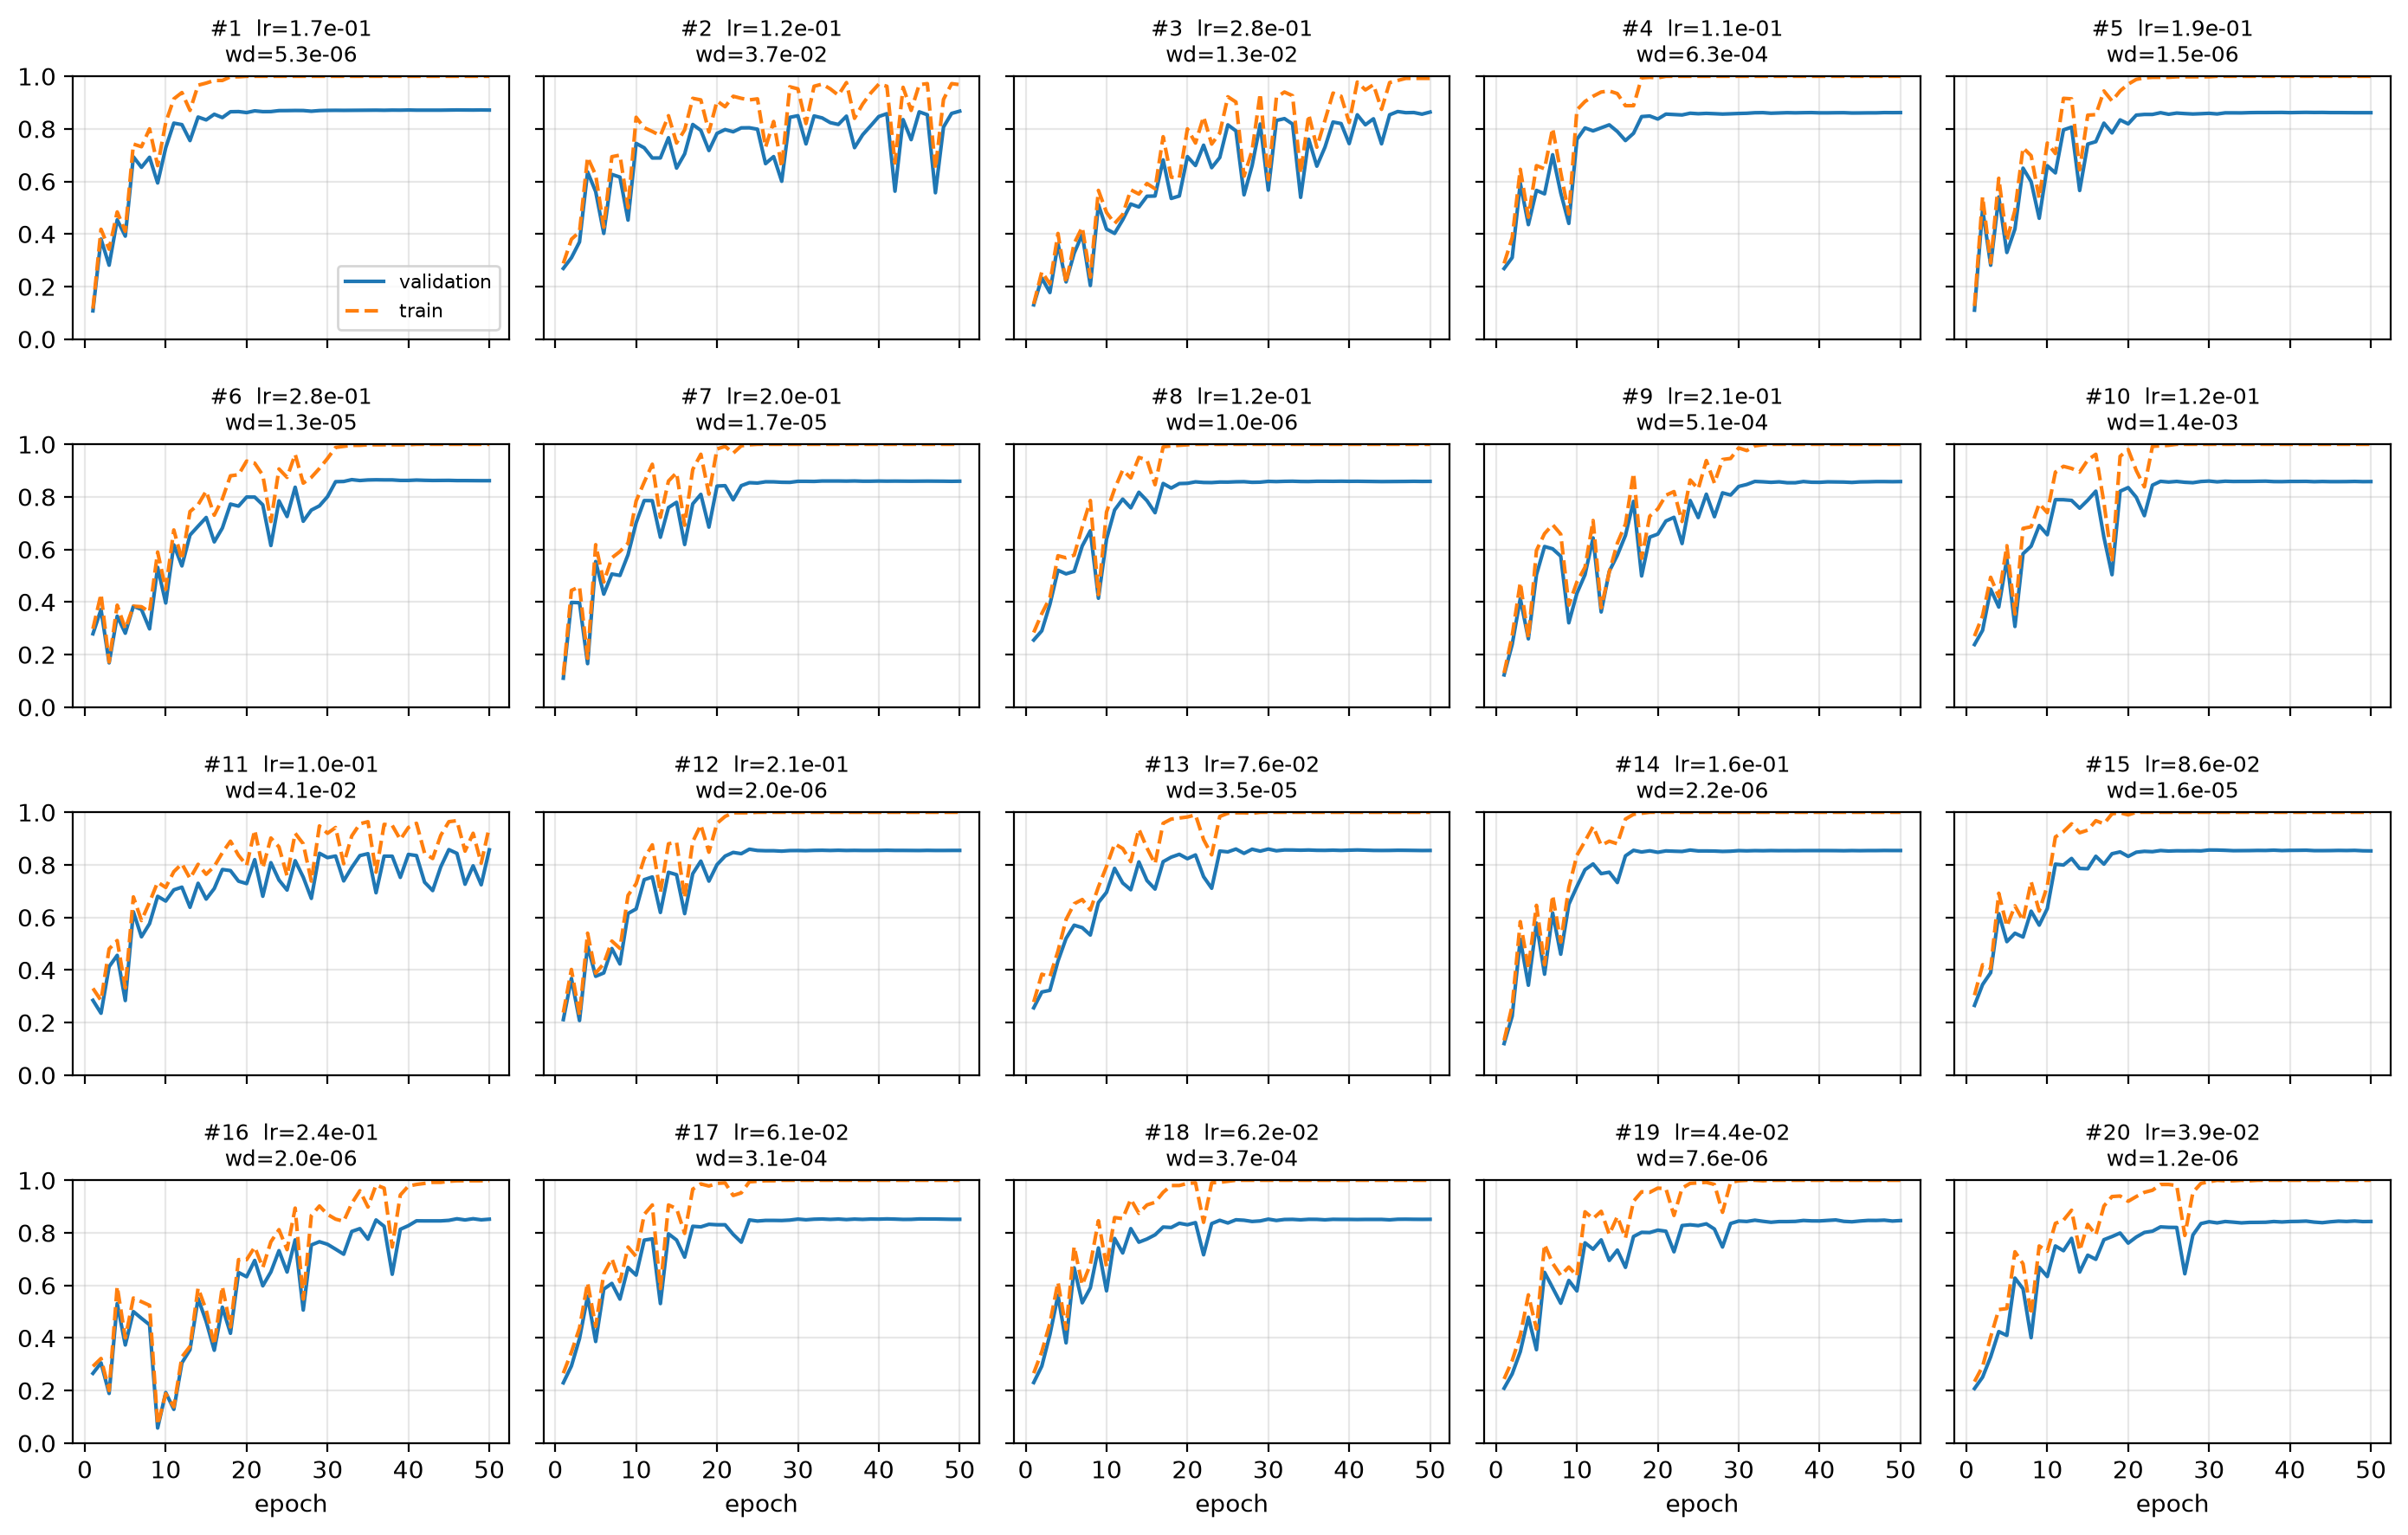
\includegraphics[height=0.56\textheight]{hyper_top20.png}
\raggedright
\small
\begin{itemize}
\item \code{plt.subplots(4, 5, sharex=True, sharey=True)}: 20칸이 같은 축 범위를 쓴다 $\to$ 비교하기 쉽다
\item 실선: 검증, 점선: 훈련. 대부분 훈련 정확도는 $100\%$, 검증은 $85$--$87\%$ $\to$ 500장이라 오버피팅
\end{itemize}
\end{frame}

\begin{frame}[fragile]{그림: 학습률--가중치 감소 평면 (\code{hyper\_scatter.png})}
\begin{columns}[T,onlytextwidth]
\begin{column}{0.48\textwidth}
\begin{lstlisting}[basicstyle=\codetiny]
fig, ax = plt.subplots(figsize=(6.5, 5))
sc = ax.scatter([r["lr"] for r in results],
                [r["wd"] for r in results],
                c=[r["val"][-1] for r in results],
                cmap="viridis", vmin=0, vmax=1, s=40)
ax.set_xscale("log")
ax.set_yscale("log")
...
fig.colorbar(sc, label="validation accuracy")
\end{lstlisting}
\footnotesize
\begin{itemize}
\item 점 하나 $=$ 시도 하나. 위치: (학습률, 가중치 감소), 색: 검증 정확도
\item \code{c=[...]}: 점마다 색을 정할 값. \code{vmin}, \code{vmax}: 색의 범위를 $0$--$1$로 고정
\item \code{colorbar}: 색과 값의 대응 막대
\end{itemize}
\end{column}
\begin{column}{0.48\textwidth}
\centering
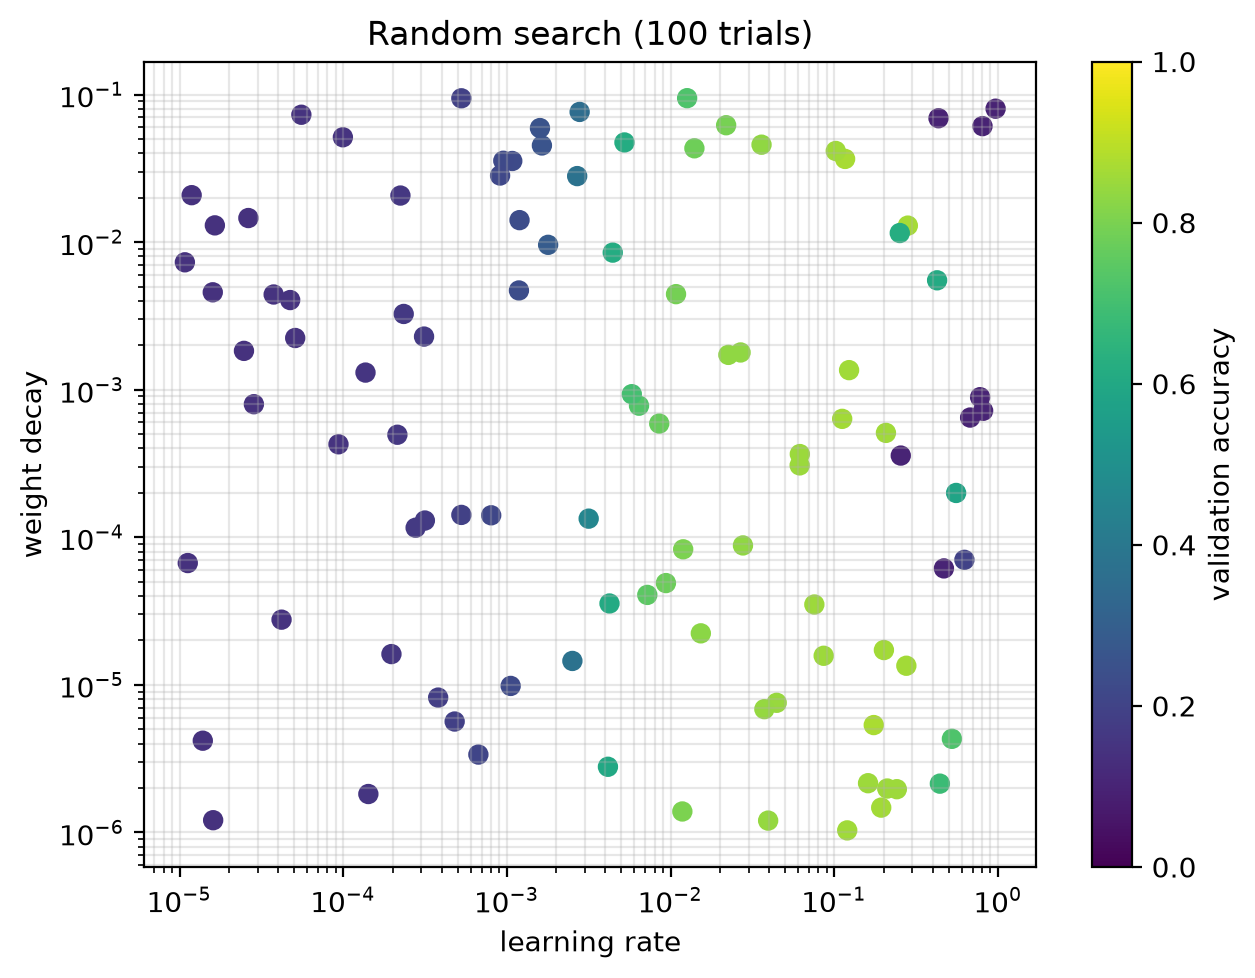
\includegraphics[width=\linewidth]{hyper_scatter.png}
\end{column}
\end{columns}
\vskip1mm
\small
\begin{itemize}
\item 색이 \textbf{가로}(학습률)로는 크게 바뀌고 \textbf{세로}(가중치 감소)로는 거의 바뀌지 않는다 $\to$ 학습률이 결과를 거의 결정한다
\end{itemize}
\end{frame}

\begin{frame}[shrink,fragile]{마지막에 한 번: test}
\small
\begin{lstlisting}
best = results[0]
net, _, _ = train(best["lr"], best["wd"])
print(f"chosen: lr {best['lr']:.2e}, weight decay {best['wd']:.2e}  ->  "
      f"validation {best['val'][-1]:.4f}, test {net.accuracy(x_test, t_test):.4f}")
\end{lstlisting}
\begin{lstlisting}[style=outstyle]
chosen: lr 1.74e-01, weight decay 5.34e-06  ->  validation 0.8714, test 0.8701
\end{lstlisting}
\begin{itemize}
\item 정렬했으므로 \code{results[0]}이 1등. 100번의 시도에서는 신경망을 저장하지 않았으므로 \textbf{다시 학습}한다
\item \code{train} 안에서 씨앗을 고정했으므로 \textbf{같은} 신경망이 다시 만들어진다
\item 검증 $87.14\%$, test $87.01\%$. 500장으로 학습한 신경망의 성능
\end{itemize}
\begin{keybox}[하이퍼파라미터 탐색의 순서]
\small
\begin{enumerate}
\item 넓은 범위에서 \textbf{로그 스케일}로 무작위로 뽑는다 (적은 데이터, 짧은 학습으로 빠르게)
\item 검증 정확도가 좋은 범위로 \textbf{좁혀서} 다시 뽑는다
\item 고른 값으로 전체 데이터를 학습하고, test는 \textbf{마지막에 한 번}
\end{enumerate}
\end{keybox}
\end{frame}

% =================================================
\section{\texttt{mnist\_torch.py}: 같은 신경망을 PyTorch로}
% =================================================

\begin{frame}{우리 코드와 PyTorch의 대응 (파일 첫머리의 주석)}
\footnotesize
\centering
\small
\footnotesize
\renewcommand{\arraystretch}{1.05}
\begin{tabular}{>{\raggedright}p{4.0cm}>{\raggedright}p{4.0cm}>{\raggedright\arraybackslash}p{4.4cm}}
\toprule
\textbf{우리 NumPy 코드} & \textbf{PyTorch} & \textbf{주의할 점} \\
\midrule
\code{Affine} & \code{nn.Linear} & 가중치가 \code{(out, in)}: 우리 $W$의 \textbf{전치} \\
\code{Relu} & \code{nn.ReLU} & \\
\code{BatchNormalization} & \code{nn.BatchNorm1d} & \code{momentum=0.1} $=$ 우리의 $0.9$ \\
\code{Dropout} & \code{nn.Dropout} & 같은 역 드롭아웃 \\
\code{SoftmaxWithCrossEntropy} & \code{nn.CrossEntropyLoss} & 정답은 one-hot이 아니라 \textbf{클래스 번호} \\
모든 계층의 \code{backward()} & \code{loss.backward()} & autograd가 그래프를 기록 \\
\code{optimizers.py} & \code{torch.optim} & \code{SGD}, \code{Adam}, \code{AdamW}, \ldots \\
\code{train\_flg=True / False} & \code{model.train() / .eval()} & 모델 전체의 모드 \\
\code{weight\_init\_std="he"} & \code{nn.init.kaiming\_normal\_} & \\
\bottomrule
\end{tabular}
\raggedright
\begin{itemize}
\item 데이터는 우리의 \code{mnist\_data.py}를 그대로 쓴다 $\to$ 훈련/검증/test 분할이 NumPy 코드와 \textbf{같다}
\item 설정도 \code{mnist\_numpy\_final.py}와 같다: He, BatchNorm, 은닉층 4개, AdamW, 15 epoch
\end{itemize}
\end{frame}

\begin{frame}[fragile]{1. import와 준비}
\begin{columns}[T,onlytextwidth]
\begin{column}{0.40\textwidth}
\begin{lstlisting}
import os
import copy
import numpy as np
import matplotlib.pyplot as plt
import torch
from torch import nn
from torch.utils.data import TensorDataset, DataLoader

from mnist_data import load_mnist_split
\end{lstlisting}
\end{column}
\begin{column}{0.57\textwidth}
\begin{lstlisting}
FIG_DIR = os.path.join(os.path.dirname(
    os.path.abspath(__file__)), "..", "figures")
os.makedirs(FIG_DIR, exist_ok=True)

torch.manual_seed(0)
device = "cuda" if torch.cuda.is_available() else "cpu"
print(f"device: {device}")
\end{lstlisting}
\begin{lstlisting}[style=outstyle]
device: cuda
\end{lstlisting}
\end{column}
\end{columns}
\small
\begin{itemize}
\item PyTorch 코드에서도 우리 모듈 \code{mnist\_data}를 import 할 수 있다 (같은 폴더의 Python 파일일 뿐)
\item \code{torch.manual\_seed(0)}: 가중치 초기화, 드롭아웃, \code{shuffle}의 난수를 고정
\item 이번 실행은 이 컴퓨터의 GPU(RTX 3050)에서 했다. GPU가 없으면 같은 코드가 \code{cpu}로 돈다
\end{itemize}
\end{frame}

\begin{frame}[fragile]{2. 데이터: NumPy 배열 $\to$ 텐서 $\to$ \code{DataLoader}}
\begin{lstlisting}
x_train, t_train, x_val, t_val, x_test, t_test = load_mnist_split()   # 55000 / 5000 / 10000

def to_dataset(x, t):
    """images (N, 784) and one-hot labels (N, 10) -> a dataset of (image, class index)"""
    return TensorDataset(torch.tensor(x, dtype=torch.float32),
                         torch.tensor(np.argmax(t, axis=1)))

train_loader = DataLoader(to_dataset(x_train, t_train), batch_size=100, shuffle=True)
val_loader = DataLoader(to_dataset(x_val, t_val), batch_size=1000)
test_loader = DataLoader(to_dataset(x_test, t_test), batch_size=1000)
\end{lstlisting}
\begin{itemize}
\item \code{dtype=torch.float32}: NumPy의 \code{float64}를 PyTorch의 기본 자료형으로
\item \code{np.argmax(t, axis=1)}: one-hot \code{(N, 10)} $\to$ 클래스 번호 \code{(N,)} (\code{int64}). \code{CrossEntropyLoss}가 요구하는 형태
\item \code{DataLoader}: 우리 코드의 \code{permutation}으로 섞고 100개씩 자르는 일을 대신한다
\item 평가용은 섞지 않고 1000개씩 (기울기가 필요 없어 메모리를 덜 쓴다)
\end{itemize}
\end{frame}

\begin{frame}[shrink,fragile]{3. 모델: \code{make\_mlp}}
\small
\begin{lstlisting}
def make_mlp(hidden=(100, 100, 100, 100), use_batchnorm=True, dropout_ratio=0.0):
    layers, n_in = [], 784
    for n_out in hidden:
        layers.append(nn.Linear(n_in, n_out))
        if use_batchnorm:
            layers.append(nn.BatchNorm1d(n_out))
        layers.append(nn.ReLU())
        if dropout_ratio > 0:
            layers.append(nn.Dropout(dropout_ratio))
        n_in = n_out
    layers.append(nn.Linear(n_in, 10))            # scores U; softmax is inside the loss
    model = nn.Sequential(*layers)
    ...
\end{lstlisting}
\small
\begin{itemize}
\item \code{MultiLayerNet.\_\_init\_\_}과 \textbf{같은 구조}: Linear $\to$ (BatchNorm) $\to$ ReLU $\to$ (Dropout)를 반복, 마지막 Linear
\item \code{nn.BatchNorm1d(n\_out)}: 노드 수만 알려 주면 $\gamma$, $\beta$, 이동평균을 스스로 만든다
\item \code{dropout\_ratio=0.0}이면 드롭아웃 계층을 넣지 않는다 (NumPy 최종 코드처럼 꺼 둔 상태)
\item \code{nn.Sequential(*layers)}: 리스트를 풀어서 순서대로 잇는다. 마지막에 softmax는 \textbf{없다}
\end{itemize}
\end{frame}

\begin{frame}[fragile]{3. He 초기화}
\begin{lstlisting}
    for m in model.modules():
        if isinstance(m, nn.Linear):
            nn.init.kaiming_normal_(m.weight, nonlinearity="relu")   # He: std = sqrt(2 / n_in)
            nn.init.zeros_(m.bias)
    return model
\end{lstlisting}
\begin{itemize}
\item \code{model.modules()}: 모델 자신과 그 안의 모든 계층을 차례로 꺼낸다
\item \code{isinstance(m, nn.Linear)}: 그중 Linear만 (BatchNorm, ReLU는 건너뛴다)
\item \code{kaiming\_normal\_}: \textbf{He 초기화} (Kaiming He는 He 초기화를 제안한 사람). 표준편차 $\sqrt{2/n_{\text{in}}}$의 정규분포
\item \code{zeros\_}: 편향을 $0$으로. 우리 코드의 \code{np.zeros((1, n\_out))}
\item 이름 끝의 \code{\_}: PyTorch에서 \textbf{제자리에서 바꾸는} 함수의 표시 (\code{x.grad.zero\_()}와 같다)
\end{itemize}
\begin{remarkbox}
\small 따로 지정하지 않으면 \code{nn.Linear}는 균등분포로 초기화한다. 여기서는 NumPy 코드와 맞추려고 He로 바꿨다.
\end{remarkbox}
\end{frame}

\begin{frame}[fragile]{3. 모델 확인}
\begin{lstlisting}
model = make_mlp().to(device)
print(model)
print("number of parameters:", sum(p.numel() for p in model.parameters()))
\end{lstlisting}
\begin{columns}[T,onlytextwidth]
\begin{column}{0.62\textwidth}
\begin{lstlisting}[style=outstyle,basicstyle=\codetiny]
Sequential(
  (0): Linear(in_features=784, out_features=100, bias=True)
  (1): BatchNorm1d(100, eps=1e-05, momentum=0.1, affine=True,
                   track_running_stats=True)
  (2): ReLU()
  (3): Linear(in_features=100, out_features=100, bias=True)
  (4): BatchNorm1d(100, eps=1e-05, momentum=0.1, ...)
  (5): ReLU()
  ...
  (11): ReLU()
  (12): Linear(in_features=100, out_features=10, bias=True)
)
number of parameters: 110610
\end{lstlisting}
\end{column}
\begin{column}{0.34\textwidth}
\small
\begin{itemize}
\item 매개변수 $110610$개: NumPy 최종 코드와 \textbf{같다}
\item \code{momentum=0.1}: 새 값의 비중. 우리 코드의 \code{0.9}는 옛 값의 비중 $\to$ \textbf{같은 뜻}
\item \code{eps=1e-05}: 우리는 $10^{-7}$ (아주 작은 차이)
\item \code{affine=True}: $\gamma$, $\beta$를 학습한다
\end{itemize}
\end{column}
\end{columns}
\end{frame}

\begin{frame}[fragile]{4. 손실 함수와 AdamW}
\begin{lstlisting}
loss_fn = nn.CrossEntropyLoss()                  # softmax + cross-entropy, averaged over the batch

# AdamW: decay only the weights W (2-D), not B, gamma, beta (1-D) -- the same choice as our code
decay = [p for p in model.parameters() if p.dim() == 2]
no_decay = [p for p in model.parameters() if p.dim() == 1]
optimizer = torch.optim.AdamW([{"params": decay, "weight_decay": 0.01},
                               {"params": no_decay, "weight_decay": 0.0}], lr=0.001)
\end{lstlisting}
\begin{itemize}
\item \code{p.dim()}: 텐서의 차원 수. Linear의 가중치는 2차원 \code{(out, in)}, 편향과 $\gamma$, $\beta$는 1차원
\item \textbf{매개변수 그룹}: \code{\{"params": ..., "weight\_decay": ...\}} 딕셔너리의 리스트. 그룹마다 다른 설정
\item 우리 \code{AdamW}가 \code{key.startswith("W")}로 한 일을 PyTorch에서는 이렇게 한다
\item 그냥 \code{AdamW(model.parameters(), weight\_decay=0.01)}로 쓰면 편향과 $\gamma$, $\beta$까지 줄어든다
\end{itemize}
\end{frame}

\begin{frame}[shrink,fragile]{5. 한 epoch 학습: \code{train\_one\_epoch}}
\small
\begin{lstlisting}
def train_one_epoch(model, loader):
    model.train()                                 # BatchNorm: batch statistics, Dropout: on
    total_loss, n = 0.0, 0
    for xb, yb in loader:
        xb, yb = xb.to(device), yb.to(device)
        loss = loss_fn(model(xb), yb)             # forward: the graph is recorded
        optimizer.zero_grad()                     # gradients ADD UP in .grad, so clear them first
        loss.backward()                           # backward: dL/dW for every parameter
        optimizer.step()                          # = optimizer.update(params, grads)
        total_loss += loss.item() * len(yb)
        n += len(yb)
    return total_loss / n
\end{lstlisting}
\small
\begin{itemize}
\item \code{model.train()}: 이번에는 \textbf{실제로 결과를 바꾼다}. BatchNorm이 미니배치 통계를 쓰고 이동평균을 갱신한다
\item 가운데 4줄: PyTorch 입문에서 본 학습 루프 그대로. NumPy의 \code{loss} $\to$ \code{backward} $\to$ \code{update}와 짝
\item \code{loss.item() * len(yb)}: 미니배치 평균 손실 $\times$ 개수 $=$ 합. 마지막에 전체 개수 \code{n}으로 나누면 \textbf{epoch 평균}
\end{itemize}
\end{frame}

\begin{frame}[fragile]{5. 평가: \code{accuracy}}
\begin{lstlisting}
@torch.no_grad()                                  # no graph needed: faster, less memory
def accuracy(model, loader):
    model.eval()                                  # BatchNorm: running averages, Dropout: off
    correct, n = 0, 0
    for xb, yb in loader:
        xb, yb = xb.to(device), yb.to(device)
        correct += (model(xb).argmax(dim=1) == yb).sum().item()
        n += len(yb)
    return correct / n
\end{lstlisting}
\begin{itemize}
\item \code{@torch.no\_grad()}: 함수 전체를 그래프 기록 없이 (데코레이터)
\item \code{model.eval()}: BatchNorm은 \textbf{이동평균}, Dropout은 끔. 우리 \code{predict(X)}의 \code{train\_flg=False}
\item \code{model.eval()}을 빠뜨리면? 평가 미니배치 1000개의 통계로 정규화된다 $\to$ 결과가 미니배치에 따라 달라진다
\item 이 함수가 모드를 평가로 바꿔 두므로, \code{train\_one\_epoch}의 첫 줄에서 다시 \code{model.train()}
\end{itemize}
\end{frame}

\begin{frame}[shrink,fragile]{6. 학습 반복과 가장 좋은 epoch 저장}
\footnotesize
\begin{lstlisting}[basicstyle=\codetiny]
epochs = 15
history = {"loss": [], "train": [], "val": []}
best_val, best_state = 0.0, None
for epoch in range(1, epochs + 1):
    history["loss"].append(train_one_epoch(model, train_loader))
    history["train"].append(accuracy(model, train_loader))
    history["val"].append(accuracy(model, val_loader))
    print(f"epoch {epoch:2d} | loss {history['loss'][-1]:.4f} | "
          f"train acc {history['train'][-1]:.4f} | val acc {history['val'][-1]:.4f}")
    if history["val"][-1] > best_val:             # keep the epoch with the best VALIDATION accuracy
        best_val, best_epoch = history["val"][-1], epoch
        best_state = copy.deepcopy(model.state_dict())
\end{lstlisting}
\small
\begin{itemize}
\item NumPy 최종 코드와 같은 흐름. 다른 곳은 마지막 줄 하나: \code{get\_state(net)} $\to$ \code{copy.deepcopy(model.state\_dict())}
\item \code{state\_dict()}에는 매개변수뿐 아니라 BatchNorm의 \code{running\_mean}, \code{running\_var}도 \textbf{들어 있다}
\begin{itemize}
\item PyTorch는 이런 값을 \textbf{버퍼}(buffer)로 등록해 둔다. 그래서 우리처럼 따로 챙길 필요가 없다
\end{itemize}
\item \code{deepcopy}: \code{state\_dict()}는 모델의 텐서를 \textbf{가리킬} 뿐이다. 복사하지 않으면 학습이 계속되며 함께 바뀐다
\end{itemize}
\end{frame}

\begin{frame}[fragile]{6. 실행 결과}
\begin{lstlisting}[style=outstyle,basicstyle=\codesmall]
epoch  1 | loss 0.2994 | train acc 0.9724 | val acc 0.9654
epoch  2 | loss 0.1074 | train acc 0.9814 | val acc 0.9704
epoch  3 | loss 0.0746 | train acc 0.9875 | val acc 0.9738
epoch  4 | loss 0.0608 | train acc 0.9914 | val acc 0.9748
epoch  5 | loss 0.0468 | train acc 0.9921 | val acc 0.9780
epoch  6 | loss 0.0414 | train acc 0.9944 | val acc 0.9782
epoch  7 | loss 0.0377 | train acc 0.9957 | val acc 0.9806
epoch  8 | loss 0.0300 | train acc 0.9960 | val acc 0.9784
epoch  9 | loss 0.0270 | train acc 0.9959 | val acc 0.9786
epoch 10 | loss 0.0260 | train acc 0.9969 | val acc 0.9802
epoch 11 | loss 0.0234 | train acc 0.9972 | val acc 0.9798
epoch 12 | loss 0.0233 | train acc 0.9975 | val acc 0.9828
epoch 13 | loss 0.0193 | train acc 0.9979 | val acc 0.9794
epoch 14 | loss 0.0182 | train acc 0.9979 | val acc 0.9814
epoch 15 | loss 0.0175 | train acc 0.9977 | val acc 0.9808
\end{lstlisting}
\small
\begin{itemize}
\item NumPy 최종 코드와 거의 같은 곡선: 첫 epoch 검증 $96.5\%$, 이후 $97.4$--$98.3\%$에서 오르내린다
\item 숫자가 똑같지는 않다: 초기 가중치와 미니배치 순서의 난수가 다르고(NumPy와 PyTorch), BatchNorm의 \code{eps}도 다르다
\end{itemize}
\end{frame}

\begin{frame}[fragile]{7. test는 한 번만}
\begin{lstlisting}
model.load_state_dict(best_state)
print(f"chosen epoch {best_epoch}: val acc {best_val:.4f}, test acc {accuracy(model, test_loader):.4f}")
# torch.save(model.state_dict(), "mnist_torch.pt")   # to keep the trained weights
\end{lstlisting}
\begin{lstlisting}[style=outstyle]
chosen epoch 12: val acc 0.9828, test acc 0.9780
\end{lstlisting}
\begin{itemize}
\item \code{load\_state\_dict}: 저장해 둔 epoch 12의 매개변수와 이동평균을 모델에 넣는다. 우리의 \code{set\_state}
\item 주석 처리한 \code{torch.save}: 파일로 저장하고 싶을 때 주석을 푼다
\end{itemize}
\vskip1mm
\centering
\small
\renewcommand{\arraystretch}{1.2}
\begin{tabular}{lccc}
\toprule
& \textbf{고른 epoch} & \textbf{검증 정확도} & \textbf{test 정확도} \\
\midrule
\code{mnist\_numpy\_final.py} (NumPy, CPU) & 12 & $98.24\%$ & $97.87\%$ \\
\code{mnist\_torch.py} (PyTorch, GPU) & 12 & $98.28\%$ & $97.80\%$ \\
\bottomrule
\end{tabular}
\end{frame}

\begin{frame}{8. 결과 그림: \code{torch\_mnist.png}}
\centering
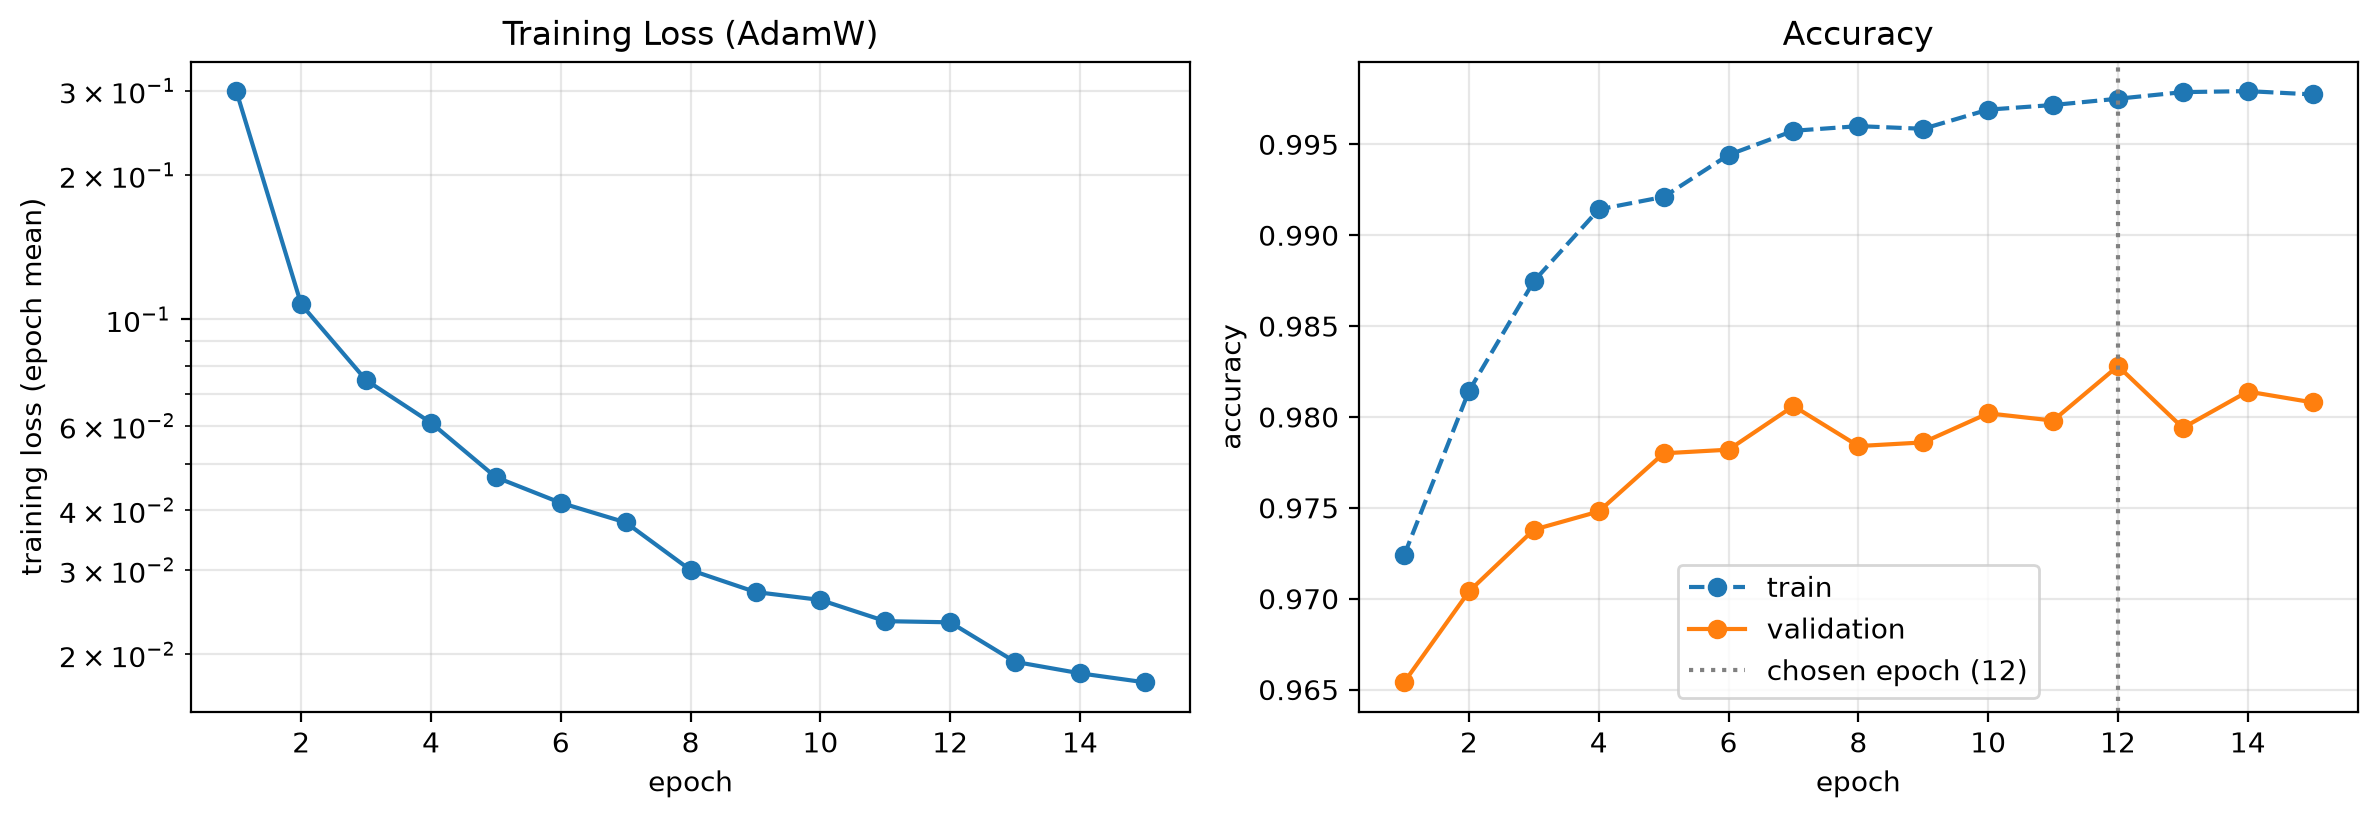
\includegraphics[width=0.92\linewidth]{torch_mnist.png}
\figcap{왼쪽: epoch 평균 손실, 오른쪽: 훈련(점선)과 검증(실선) 정확도, 회색 점선: 고른 epoch}
\raggedright
\small
\begin{itemize}
\item 그림 코드는 NumPy 최종 코드와 \textbf{같다} (\code{history} 딕셔너리의 구조도 같게 만들었다)
\item 두 프로그램이 같은 일을 한다는 것을 그림으로도 확인할 수 있다
\end{itemize}
\end{frame}

\begin{frame}{NumPy 최종 코드와 PyTorch 코드: 한 줄씩 비교}
\centering
\footnotesize
\renewcommand{\arraystretch}{1.25}
\begin{tabular}{>{\raggedright}p{2.4cm}>{\raggedright}p{5.4cm}>{\raggedright\arraybackslash}p{5.2cm}}
\toprule
\textbf{단계} & \textbf{\code{mnist\_numpy\_final.py}} & \textbf{\code{mnist\_torch.py}} \\
\midrule
데이터 & 배열 그대로, \code{permutation}으로 섞기 & \code{TensorDataset}, \code{DataLoader} \\
정답 & one-hot \code{(N, 10)} & 클래스 번호 \code{(N,)} \\
모델 & \code{MultiLayerNet(..., weight\_init\_std="he", use\_batchnorm=True)} & \code{make\_mlp()}: \code{nn.Sequential} + \code{kaiming\_normal\_} \\
최적화 & \code{AdamW(lr, weight\_decay)}: \code{W}만 감소 & \code{torch.optim.AdamW}, 매개변수 그룹 \\
학습 모드 & \code{net.loss}가 \code{train\_flg=True} & \code{model.train()} \\
한 걸음 & \code{loss}, \code{backward()}, \code{update} & \code{zero\_grad()}, \code{backward()}, \code{step()} \\
평가 모드 & \code{net.accuracy}가 \code{train\_flg=False} & \code{model.eval()} + \code{no\_grad} \\
저장 & \code{get\_state}: \code{params} + 이동평균 & \code{deepcopy(state\_dict())} \\
되돌리기 & \code{set\_state}: \code{[...]}로 제자리 복사 & \code{load\_state\_dict} \\
\bottomrule
\end{tabular}
\vskip2mm
\raggedright
\small
\begin{itemize}
\item 구조는 \textbf{같다}. PyTorch가 대신해 주는 것: 역전파, 갱신 규칙, 미니배치, 상태 저장, GPU
\end{itemize}
\end{frame}

% =================================================
\section{정리와 실습}
% =================================================

\begin{frame}{정리}
\begin{keybox}[이번 시간의 핵심]
\footnotesize
\begin{itemize}\setlength{\itemsep}{0.5mm}
\item \textbf{\code{optimizers.py}}: 모든 기법이 \code{update(params, grads)} 하나. 상태($v$, $h$, $m$)는 첫 호출 때 \code{params}와 같은 모양으로 만든다. AdamW는 Adam을 상속해 $W$만 줄인다
\item \textbf{\code{layers.py}}: BatchNorm은 학습 때 미니배치 통계, 추론 때 이동평균. 이동평균은 \code{params}에 없다. Dropout은 학습 때만 끄고 $1/\text{keep}$배
\item \textbf{최종 코드}: He + BatchNorm + AdamW, 검증 정확도가 가장 좋은 epoch를 저장, test는 한 번 $\to$ test $97.87\%$
\item \textbf{공정한 비교}: \code{seed(1)}로 같은 초기 가중치, \code{seed(2)}로 같은 미니배치. 바꾸는 것은 \textbf{하나}
\item \textbf{실험 결과}: SGD보다 Momentum, AdaGrad, Adam이 빠르다. ReLU에는 He. BatchNorm은 초기화에 덜 민감하게 한다.
규제는 너무 세면 과소적합. 학습률이 가장 중요한 하이퍼파라미터
\item \textbf{PyTorch}: 같은 구조, 같은 결과 (test $97.80\%$). \code{state\_dict}에 이동평균까지 들어 있다
\end{itemize}
\end{keybox}
\end{frame}

\begin{frame}[shrink]{실습 문제}
\small
\small
\begin{enumerate}
\item \code{mnist\_numpy\_final.py}에서 \code{use\_dropout=True}로 바꾸면 훈련과 검증 정확도의 차이는 어떻게 되는가?
\item \code{get\_state}에서 BatchNorm의 이동평균을 저장하지 \textbf{않도록} 고치고, 마지막 검증 정확도가 epoch 12의 값과 같은지 확인하기
\item 최종 코드의 \code{AdamW}를 \code{SGD(lr=0.01)}, \code{Momentum(lr=0.01)}, \code{Adam(lr=0.001)}로 바꿔 15 epoch 뒤의 검증 정확도 비교하기
\item \code{mnist\_optimizer\_compare.py}에 \code{RMSProp(lr=0.001)}을 다섯 번째 기법으로 넣어 비교하기
\item \code{weight\_init\_activation.py}에서 층을 10개로 늘리면 ReLU + Xavier의 마지막 층 표준편차는 얼마가 되는가? 먼저 예측해 보자
\item \code{mnist\_overfit.py}의 (4)에 $\lambda=0.003$, $0.05$를 더하고 검증 정확도가 가장 좋은 $\lambda$를 다시 찾기
\item \code{hyperparameter\_search.py}의 탐색 범위를 학습률 $0.03$--$0.3$으로 좁혀 다시 탐색하기
\item \code{mnist\_torch.py}에서 \code{accuracy}의 \code{model.eval()}을 지우면 검증 정확도가 어떻게 되는가? 이유는?
\end{enumerate}
\end{frame}

\end{document}
